\documentclass[dvipsnames,12pt]{report}

\usepackage{amssymb}
\usepackage{pifont}
\usepackage{amsmath}
\usepackage{graphicx}
\usepackage{multicol}
\usepackage{subfig}
\usepackage{lscape}
\usepackage{float}
\usepackage[colorinlistoftodos]{todonotes}
\usepackage[document]{ragged2e}
\usepackage{titlesec}
\titleformat{\section}[hang]{\normalfont\Large\bfseries\raggedright}{\thesection}{1em}{}
\titleformat{\subsection}[hang]{\normalfont\large\bfseries\raggedright}{\thesubsection}{1em}{}
\titleformat{\subsubsection}[hang]{\normalfont\normalsize\bfseries\raggedright}{\thesubsubsection}{1em}{}
\usepackage{tikz}
\usepackage{dirtytalk}
\usetikzlibrary{shapes.geometric, arrows}
\usepackage[utf8]{inputenc}
\usepackage{multirow}
\usepackage{datetime}
\newdateformat{monthyeardate}{%
  \monthname[\THEMONTH], \THEYEAR}
\usepackage[english]{babel}
\usepackage{wrapfig}
\usepackage{rotating}
\usepackage{epstopdf}
\usepackage{algorithm}
\usepackage{algpseudocode}
\usepackage{pdfpages}
\usepackage{hyperref}
\usepackage{booktabs}
\usepackage{array}
\usepackage{longtable}
\usepackage{setspace}
\usepackage{fancyhdr}
\usepackage{enumitem}

\pagestyle{fancy}
\raggedbottom
\fancyhead{}
\bibliographystyle{IEEEtran}

%% --- Page dimensions (updated for equal top & bottom margins) ---
\usepackage[a4paper, top=1in, bottom=1in, left=1.25in, right=1in]{geometry}

%% --- Spacing ---
\setstretch{1}
\setlength{\parskip}{3pt plus 1pt minus 1pt}
\setlength{\parindent}{0pt}

%% --- Table row height ---
\renewcommand{\arraystretch}{1.2}

%% --- Student / project details ---
\def\mytitle{SMART PLACEMENT PREPARATION PLATFORM (PREPSMART)}
\def\myname{Mala Neeraj Srinivas}
\def\mydegree{Computer Science and Engineering}
\def\mysupervisor{Dr. Prarthana Jagat Mehta}
\def\myexaminer{Dr. Reema Patel}
\def\myindustrysupervisor{Akhilesh Reddy Karra}
\def\myrollno{UI21CSC35}
\def\mydep{Computer Science and Engineering}
\def\mydegreedate{5\textsuperscript{th} July, 2026}
\def\myorganisation{Architect - Application (AuroPro Soft Systems Pvt Ltd), Hyderabad}

\setlength{\marginparwidth}{2cm}

\newcommand{\cmark}{\ding{51}}
\newcommand{\xmark}{\ding{55}}

\begin{document}
    \setlength{\parindent}{0pt}
    \baselineskip=18pt plus1pt
    \setcounter{secnumdepth}{3}
    \setcounter{tocdepth}{3}
    \pagenumbering{roman}

    \thispagestyle{empty}
\begingroup\centering
    { \Large {\bfseries \textcolor{black}{{\mytitle}} \par}}
\vspace{0.5cm}
    {\normalsize \textcolor{violet}{Submitted for the Partial Fulfillment of the}}\
    {\normalsize \textcolor{violet}{Requirements for the degree of Bachelor of Technology}}\par
\vspace{0.2cm}
    {\normalsize \textit{in} \par}
\vspace{0.2cm}
    {\large \bf \textcolor{violet}{\mydep}\par} 
\vspace{0.2cm}
    {\normalsize \textit{by} \par}
\vspace{0.2cm}
    {{\large {\bf \textcolor{ForestGreen}{\myname} \\ \textcolor{red}{Roll No.: \myrollno}}} \par}
\vspace{0.2cm}
    {\textcolor{violet}{Under the guidance of}\par}
\vspace{0.1cm}
    {\normalsize \textit{External Supervisor}\par}
\vspace{0.1cm}
    {{\large \bf \textcolor{ForestGreen}{\myindustrysupervisor}} \par}
\vspace{0.05cm}
    {\normalsize \myorganisation \par}
\vspace{0.2cm}
    {\normalsize \textit{Faculty Supervisor}\par}
\vspace{0.1cm}
    {{\large \bf \textcolor{ForestGreen}{\mysupervisor}} \par}
\vspace{0.2cm}
    {\normalsize \textit{Faculty Examiner}\par}
\vspace{0.1cm}
    {{\large \bf \textcolor{ForestGreen}{\myexaminer}} \par}
\vspace{0.2cm}
    {\begin{figure}[!h] 
	\centering
	
\includegraphics[width=30mm]{Formalities/IIIT_Surat_logo.jpg} 
     \end{figure}
    }
\vspace{1\baselineskip}
{\small \bf \textcolor{cyan}{DEPARTMENT OF \MakeUppercase{\mydep}} \par}
\vspace*{0.5ex}
{\small \bf May, 2026\par}
{\small \bf \textcolor{red}{\uppercase{Indian Institute of Information Technology Surat}-394190}}
\endgroup


    \phantomsection
    \addcontentsline{toc}{chapter}{Certificate}
    \thispagestyle{plain}
\begin{center}
{\Large\bfseries\textcolor{red}{Indian Institute of Information Technology Surat}\\[4pt]
Computer Science and Engineering Department}
\end{center}

\vspace{0.2cm}

\begin{center}

\includegraphics[width=32mm]{Formalities/IIIT_Surat_logo.jpg}
\end{center}

\vspace{0.2cm}

\begin{center}
{\Large\bfseries\uppercase{Certificate}}
\end{center}

\vspace{0.2cm}
\justify

\noindent This is to certify that the candidate \textbf{\myname} bearing Roll No.\ \textbf{\myrollno} of B.Tech.\ IV Year, 8th Semester, has successfully carried out the major project work titled

\vspace{0.2cm}
\begin{center}
``\textbf{SMART PLACEMENT PREPARATION PLATFORM (PREPSMART)}''
\end{center}
\vspace{0.2cm}

\noindent as an Industry Internship at \textbf{AuroPro Soft Systems Pvt Ltd, Hyderabad}, in partial fulfillment of the requirements for the degree of \textbf{Bachelor of Technology} in \textbf{Computer Science and Engineering Department} at \textbf{IIIT Surat}, completed in \textbf{May, 2026}.

\vspace{1cm}

\noindent\begin{tabular}{@{}p{0.5\textwidth}p{0.5\textwidth}@{}}
Faculty Supervisor: & Signature:\\[12pt]
\textbf{\mysupervisor} & \underline{\hspace{5cm}}\\[0.5cm]
Examiner : & Signature:\\[12pt]
\textbf{\myexaminer} & \underline{\hspace{5cm}}\\[0.5cm]
Director, IIIT Surat: & Signature:\\[12pt]
 & \underline{\hspace{5cm}}\\
\end{tabular}

\vspace{0.2cm}
\begin{flushright}
{\small (Seal of the Institute)}
\end{flushright}
\newpage


    \phantomsection
    \addcontentsline{toc}{chapter}{Declaration}
    \thispagestyle{plain}

\begin{center}
{\Large\bfseries\uppercase{Declaration}}
\end{center}

\vspace{1cm}

\noindent I hereby declare that:

\vspace{0.4cm}

\noindent (i)\quad This report comprises my original work towards the degree of Bachelor of Technology in Computer Science and Engineering at the Indian Institute of Information Technology (IIIT) Surat, and has not been submitted elsewhere for a degree.

\vspace{0.6cm}

\noindent (ii)\quad Due acknowledgement has been made in the text to all other material used.

\vspace{3cm}

\begin{flushright}
\textbf{\myname}\\[4pt]
Roll No.:\myrollno \\[4pt]
B.Tech.\ IV Year, CSE\\[4pt]
IIIT Surat\\[4pt]
May, 2026\\[1cm]
Signature: \underline{\hspace{4cm}}
\end{flushright}
\newpage


    \phantomsection
    \addcontentsline{toc}{chapter}{Acknowledgements}
    \thispagestyle{plain}

\begin{center}
{\Large\bfseries\uppercase{Acknowledgements}}
\end{center}

\vspace{0.8cm}

I would like to express my sincere gratitude to everyone who contributed to the successful completion of this internship and the preparation of this report.

\vspace{0.2cm}

I would like to express my heartfelt thanks to my Internship Mentor (External Supervisor), \textbf{Akhilesh Reddy Karra}, Architect - Application, and \textbf{Harathi Jayampu}, Jr. Project Manager, at \textbf{AuroPro Soft Systems Pvt Ltd}, for their invaluable guidance, continuous support, and insightful suggestions throughout the development of this project. Their practical insights and industry perspective greatly contributed to shaping this work.

\vspace{0.2cm}

I am equally grateful to my Faculty Supervisor, \textbf{Dr. Kaustubh Dhondge}, Associate Dean (Academics), for his constant encouragement, academic guidance, and support during the course of this project. His mentorship played a crucial role in the successful completion of this work.

\vspace{0.2cm}

I would also like to thank my Faculty Examiner, \textbf{Dr. Reema Patel}, Assistant Professor, for her valuable feedback and suggestions, which helped in improving the quality of this project.

\vspace{0.2cm}

I would like to extend my sincere thanks to \textbf{Polukanti Ravi Kumar} and \textbf{Chitukuru Nalini} for their continuous support and encouragement throughout this journey. Their motivation played an important role in the successful completion of this work.

\vspace{0.2cm}

I also thank the faculty and staff of the \textbf{Department of Computer Science and Engineering, Indian Institute of Information Technology Surat}, for providing me with the academic foundation to pursue this project.

\vspace{0.2cm}

I would also like to express my sincere gratitude to the \textbf{Director, Indian Institute of Information Technology Surat}, for the institutional support and for fostering an environment that encourages students to undertake impactful industry internships.

\vspace{1.5cm}

\begin{flushright}
\textbf{\myname}\\[4pt]
Roll No.: \myrollno \\[4pt]
B.Tech.\ IV Year, CSE\\[4pt]
IIIT Surat, May 2026
\end{flushright}

\newpage

    \phantomsection
    \addcontentsline{toc}{chapter}{Abstract}
    \thispagestyle{plain}

\begin{center}
{\Large\bfseries\uppercase{Abstract}}
\end{center}

\vspace{0.5cm}

The \textbf{Smart Placement Preparation Platform (PrepSmart)} is a comprehensive web-based system designed to streamline and enhance the placement preparation process for students. With increasing competition in campus placements, students require a structured, data-driven, and unified approach to preparation, which is often lacking in traditional methods.

\vspace{0.5cm}

The proposed system integrates multiple components such as \textbf{structured learning paths, coding practice, mock tests, AI-based interview simulation,} and \textbf{performance analytics} into a single platform. This eliminates the need for using multiple disconnected tools and enables a more efficient and consistent preparation strategy.

\vspace{0.5cm}

The platform is developed using \textbf{React} for the frontend, \textbf{Django REST Framework (DRF)} for backend services, and \textbf{MySQL} as the database. Secure user authentication is implemented using \textbf{JSON Web Tokens (JWT)}. The system also includes a real-time Python code execution environment, allowing users to write, run, and test code within the platform.

\vspace{0.5cm}

The backend performs analytical computations such as \textbf{accuracy tracking, weak topic identification,} and \textbf{progress monitoring,} helping users make data-driven improvements. The AI Interview module simulates interview scenarios and evaluates user responses to enhance both technical and communication skills.

\vspace{0.5cm}

The system is designed with a \textbf{modular and scalable architecture,} making it suitable for future enhancements such as cloud deployment, advanced AI recommendations, and company-specific preparation modules.

\vspace{0.5cm}

Overall, \textbf{PrepSmart} transforms traditional placement preparation into a \textbf{structured, interactive, and measurable process,} significantly improving learning efficiency and readiness for real-world interviews.

\vspace{0.5cm}

\newpage


    \phantomsection
    \tableofcontents
    \protect

    \phantomsection
    \addcontentsline{toc}{chapter}{List of Abbreviations and Acronyms}
    \thispagestyle{plain}

\begin{center}
{\Large\bfseries List of Abbreviations and Acronyms}
\end{center}

\vspace{1cm}

\begin{tabbing}
\hspace{2.5cm}\=\kill
\textbf{AI}   \> Artificial Intelligence \\[4pt]
\textbf{API}   \> Application Programming Interface \\[4pt]
\textbf{DRF}   \> Django REST Framework \\[4pt]
\textbf{DB}   \> Database \\[4pt]
\textbf{UI}   \> User Interface \\[4pt]
\textbf{UX}   \> User Experience \\[4pt]
\textbf{JWT}   \> JSON Web Token \\[4pt]
\textbf{SQL}   \> Structured Query Language \\[4pt]
\textbf{HTTP}   \> HyperText Transfer Protocol \\[4pt]
\textbf{HTML}   \> HyperText Markup Language \\[4pt]
\textbf{CSS}   \> Cascading Style Sheets \\[4pt]
\textbf{JS}   \> JavaScript \\[4pt]
\textbf{CRUD}   \> Create, Read, Update, Delete \\[4pt]
\textbf{IDE}   \> Integrated Development Environment \\[4pt]
\textbf{NLP}   \> Natural Language Processing \\[4pt]
\end{tabbing}

\newpage


    \phantomsection
    \addcontentsline{toc}{chapter}{List of Figures}
    \listoffigures

    \addcontentsline{toc}{chapter}{List of Tables}
    \listoftables

    \clearpage
    \pagenumbering{arabic}

    \chapter{Introduction}

\section{Introduction}

Campus placement is one of the most important milestones in a student's academic journey as it marks the transition from higher education to the professional world. In today's competitive recruitment environment, organizations expect graduates to possess strong programming skills, sound knowledge of core computer science subjects, analytical thinking, communication abilities, practical project experience, and problem-solving capabilities. Consequently, placement preparation has become a continuous process that requires students to develop multiple competencies simultaneously rather than focusing solely on academic performance.

With the rapid growth of online learning platforms, students now have access to a vast collection of educational resources for coding practice, aptitude preparation, interview guidance, resume building, and technical learning. Although these platforms have improved accessibility to learning materials, they generally focus on individual aspects of placement preparation and operate independently. Students are therefore required to switch between multiple applications throughout their preparation journey, making it difficult to maintain consistency, monitor progress, and evaluate their overall readiness for campus recruitment.

Most existing preparation methods lack a unified mechanism for combining learning, assessments, coding practice, interview preparation, and analytical feedback within a single environment. As a result, students often spend considerable time managing different resources instead of concentrating on continuous learning and skill improvement. Furthermore, the absence of centralized progress tracking limits their ability to identify weak areas and plan effective preparation strategies.

To address these challenges, this project presents \textbf{PrepSmart: Design and Development of a Smart Placement Preparation Platform}, a comprehensive web-based application that integrates the essential components of placement preparation into a single ecosystem. The platform provides structured learning paths, topic-wise assessments, coding practice, AI-assisted interview preparation, company-specific preparation, resume and portfolio management, personalized dashboards, and analytical performance tracking. By consolidating these functionalities into one platform, PrepSmart enables students to prepare in a structured, measurable, and efficient manner.

The application is developed using modern full-stack technologies, with React for the frontend, Django and Django REST Framework (DRF) for backend development, and MySQL as the database management system. Secure authentication is implemented using JSON Web Tokens (JWT), while RESTful APIs facilitate seamless communication between different components of the system. The modular architecture adopted by the platform ensures scalability, maintainability, and flexibility for future enhancements.

Overall, PrepSmart aims to simplify the placement preparation process by providing students with an integrated platform that supports learning, practice, assessment, performance analysis, and career development. The proposed system improves preparation efficiency, reduces dependency on multiple applications, and provides continuous analytical feedback to enhance students' employability and placement readiness.

\section{Problem Statement}

The placement preparation process has become increasingly complex due to the growing expectations of recruiters and the availability of numerous independent learning resources. Students are expected to prepare for aptitude tests, programming assessments, technical interviews, behavioral interviews, resume screening, and company-specific recruitment processes within a limited period. However, the absence of a unified preparation platform often forces students to depend on multiple applications and websites to accomplish these tasks.

Existing platforms generally specialize in only one aspect of placement preparation. Coding platforms focus on programming practice, learning platforms provide theoretical content, interview platforms emphasize interview experiences, and resume builders assist in resume creation. Since these services operate independently, students must repeatedly switch between platforms, resulting in fragmented learning, inconsistent preparation strategies, and difficulty in monitoring their overall progress.

Another major limitation is the lack of comprehensive performance analytics. Most available systems provide isolated metrics such as coding scores or quiz results but fail to present a consolidated view of a student's placement readiness. Consequently, students often find it difficult to identify weak areas, evaluate their preparation status, and prioritize topics requiring additional attention.

Furthermore, many existing systems offer limited personalization and do not effectively support company-specific preparation. Students preparing for different organizations often need to manually collect interview experiences, recruitment patterns, aptitude questions, and technical resources from multiple sources, making the preparation process inefficient and time-consuming.

Therefore, there is a need for a centralized, intelligent, and scalable platform that integrates learning resources, coding practice, assessments, interview preparation, resume management, portfolio development, and analytical dashboards within a single application. Such a platform should enable students to prepare systematically, continuously monitor their progress, and make data-driven improvements throughout their placement journey. PrepSmart has been developed to address these challenges by providing an integrated ecosystem for comprehensive placement preparation.

\section{Objectives}

The primary objective of PrepSmart is to design and develop a comprehensive web-based placement preparation platform that integrates learning, assessment, coding practice, interview preparation, and performance analysis within a single application. The platform aims to simplify the placement preparation process while enabling students to continuously monitor their progress and improve their overall employability.

The specific objectives of the proposed system are as follows:

\begin{enumerate}
    \item To develop a centralized platform that combines various placement preparation activities into a unified environment.

    \item To provide structured learning paths covering aptitude, programming, computer science fundamentals, interview preparation, and company-specific learning resources.

    \item To implement coding practice with an integrated code editor and execution support for improving programming skills.

    \item To design and develop mock tests, quizzes, and assessment modules for continuous evaluation of student performance.

    \item To provide AI-assisted interview preparation that enables students to practice interview scenarios and improve their communication and technical skills.

    \item To implement secure user authentication and profile management using JSON Web Tokens (JWT).

    \item To provide personalized dashboards that present learning progress, coding performance, assessment scores, and placement readiness through analytical visualizations.

    \item To maintain resume and portfolio information within the platform, allowing students to organize their professional profiles for placement activities.

    \item To adopt a modular software architecture that supports scalability, maintainability, and future enhancements.

    \item To develop a user-friendly, responsive, and interactive web application using modern full-stack technologies.
\end{enumerate}

\section{Scope of the Project}

PrepSmart is designed as a comprehensive web-based placement preparation platform that integrates multiple activities involved in campus recruitment into a single application. The project focuses on simplifying the preparation process by providing structured learning resources, coding practice, assessments, interview preparation, and performance analysis through a unified and user-friendly interface.

The scope of the project is categorized as follows:

\subsection*{Functional Scope}

The platform provides the following core functionalities:

\begin{itemize}
    \item User registration, login, and profile management.
    \item Structured learning paths for placement preparation.
    \item Topic-wise quizzes and mock tests.
    \item Integrated coding workspace with code execution support.
    \item AI-assisted interview preparation.
    \item Company-specific preparation modules.
    \item Resume and portfolio management.
    \item Personalized dashboard with progress analytics.
    \item Daily goals and preparation tracking.
\end{itemize}

\subsection*{Technical Scope}

The system is developed as a modern full-stack web application using React for the frontend and Django with Django REST Framework (DRF) for backend services. RESTful APIs facilitate communication between system components, while JSON Web Tokens (JWT) provide secure authentication and authorization. The modular architecture enables scalability, maintainability, and easy integration of future features.

\subsection*{Future Scope}

Although the current implementation provides a complete placement preparation environment, the platform has been designed to support future enhancements. Potential improvements include:

\begin{itemize}
    \item AI-based personalized learning recommendations.
    \item Cloud deployment for improved scalability.
    \item Support for multiple programming languages in the coding environment.
    \item Integration with online coding platforms and recruitment portals.
    \item Mobile application support.
    \item Advanced analytics and recruiter dashboards.
\end{itemize}

\section{Proposed Methodology}

The development of PrepSmart follows a structured Software Development Life Cycle (SDLC) approach to ensure systematic planning, design, implementation, testing, and deployment. The methodology adopted for the project consists of the following phases:

\begin{enumerate}
    \item \textbf{Requirement Analysis:} The functional and non-functional requirements were identified through an analysis of existing placement preparation platforms and discussions with students to understand the challenges faced during placement preparation.

    \item \textbf{System Design:} Based on the identified requirements, the overall software architecture, database schema, module structure, user interfaces, and API design were planned. UML diagrams and database models were prepared to provide a clear blueprint for implementation.

    \item \textbf{Implementation:} The frontend was developed using React to provide a responsive and interactive user interface, while the backend was implemented using Django and Django REST Framework (DRF). RESTful APIs were developed to facilitate communication between the frontend and backend. JSON Web Tokens (JWT) were used to implement secure authentication and authorization.

    \item \textbf{Database Development:} The database was designed to efficiently manage user profiles, learning resources, coding activities, assessments, interview records, and analytical data while ensuring data integrity and scalability.

    \item \textbf{Integration and Testing:} Individual modules were integrated into a unified system and tested using unit testing, integration testing, and functional testing to ensure correctness, reliability, and seamless interaction among system components.

    \item \textbf{Evaluation:} The completed platform was evaluated by verifying its core functionalities, user experience, security, and overall performance to ensure that the project objectives were successfully achieved.
\end{enumerate}

\section{Organization of the Report}

This report is organized into seven chapters. Chapter 1 introduces the project, defines the problem statement, presents the objectives, scope, and development methodology. Chapter 2 reviews existing literature and analyzes current placement preparation platforms to identify research gaps. Chapter 3 discusses the system analysis and design, including requirement analysis, software architecture, database design, and UML diagrams. Chapter 4 presents the implementation details of the proposed system, describing the technologies used and the development of individual modules. Chapter 5 discusses the experimental results, system features, and performance analysis. Chapter 6 presents the testing strategy, validation techniques, and test results. Finally, Chapter 7 summarizes the project, highlights its contributions, discusses limitations, and outlines possible future enhancements.

    \chapter{Literature Survey}

\section{Introduction}

The literature survey is an essential phase of software development that involves studying existing systems, research contributions, and technologies related to the proposed project. It helps in understanding current approaches, identifying their strengths and limitations, and recognizing the research gap that motivates the development of a new solution. For the PrepSmart platform, the literature survey focuses on modern placement preparation platforms, online learning systems, coding practice portals, interview preparation resources, and educational technologies that support campus recruitment.

Over the past decade, digital learning platforms have significantly transformed placement preparation by providing students with online coding environments, structured learning materials, mock assessments, interview experiences, and skill development resources. These platforms have improved accessibility to quality educational content and enabled students to prepare independently from any location. However, most existing systems focus on specific aspects of placement preparation rather than providing a unified learning ecosystem.

Students preparing for campus recruitment typically rely on multiple platforms for coding practice, aptitude preparation, interview guidance, resume development, and progress tracking. This fragmented approach often results in inconsistent preparation, inefficient resource management, and difficulty in evaluating overall placement readiness. Furthermore, many platforms provide limited personalization and lack integrated analytical features that help students identify strengths and weaknesses throughout their preparation journey.

The objective of this chapter is to examine widely used placement preparation platforms, analyze their features, identify their limitations, and establish the necessity for a comprehensive platform such as PrepSmart. The findings of this survey provide the foundation for the design and development decisions presented in the subsequent chapters.

\section{Review of Existing Placement Preparation Platforms}

The increasing demand for technical skills has resulted in the emergence of several online platforms that support placement preparation. These platforms provide resources such as programming challenges, interview experiences, technical articles, aptitude questions, and online courses. Although they have significantly improved accessibility to educational content, most of them focus on specific aspects of placement preparation rather than providing a comprehensive solution. The following subsections present a review of widely used placement preparation platforms.

\subsection{LeetCode}

LeetCode is one of the most widely used online coding platforms for technical interview preparation. It provides a large collection of programming problems covering data structures, algorithms, databases, system design, and competitive programming. The platform also offers company-specific interview questions, coding contests, and discussion forums that help students prepare for software engineering interviews.

Despite its extensive collection of coding problems, LeetCode primarily focuses on programming practice and interview questions. It does not provide aptitude preparation, resume management, personalized learning paths, interview simulations, or integrated placement analytics, requiring students to depend on additional platforms for complete preparation.

\subsection{HackerRank}

HackerRank is an online platform designed for programming practice, skill assessment, and technical recruitment. It supports multiple programming languages and provides challenges related to algorithms, databases, artificial intelligence, and software development. Organizations also use HackerRank to conduct online coding assessments during recruitment.

Although HackerRank offers an excellent environment for coding practice and technical assessments, it provides limited support for interview preparation, learning progress analysis, resume management, and company-specific preparation. Students must therefore combine HackerRank with other learning resources to prepare comprehensively.

\subsection{GeeksforGeeks}

GeeksforGeeks is a popular educational platform that provides tutorials, interview preparation articles, coding questions, aptitude resources, and explanations of computer science concepts. It serves as a valuable reference for students preparing for technical interviews by offering extensive theoretical content and programming tutorials.

However, GeeksforGeeks primarily functions as a learning resource rather than an integrated placement preparation platform. Features such as personalized dashboards, structured preparation tracking, AI-assisted interview practice, and unified progress monitoring are limited.

\subsection{InterviewBit}

InterviewBit focuses on technical interview preparation through guided learning paths, coding exercises, and interview-oriented programming questions. The platform emphasizes structured learning and provides company-specific interview experiences that assist students in understanding real recruitment processes.

While InterviewBit offers organized learning content and coding practice, it lacks several complementary features such as resume management, portfolio development, AI-assisted interviews, integrated analytics, and comprehensive placement tracking.

\subsection{LinkedIn Learning}

LinkedIn Learning is an online educational platform offering professional courses across technology, business, communication, and leadership domains. Students can access expert-led video courses to strengthen both technical and soft skills required for career development.

Although LinkedIn Learning provides high-quality educational content, it is not specifically designed for placement preparation. It does not include integrated coding practice, mock assessments, company-specific preparation, or placement performance analytics within a unified platform.

\section{Comparative Analysis of Existing Platforms}

Table \ref{tab:comparison} presents a comparative analysis of widely used placement preparation platforms based on important features required during campus recruitment. The comparison highlights that while existing platforms perform well in specific domains such as coding practice or technical learning, none of them provide a unified ecosystem that integrates learning, assessments, coding practice, interview preparation, resume management, and analytical performance tracking within a single application.

\begin{table}[H]
\centering
\caption{Comparison of Existing Placement Preparation Platforms}
\label{tab:comparison}
\renewcommand{\arraystretch}{1.25}
\resizebox{\textwidth}{!}{
\begin{tabular}{|p{5cm}|c|c|c|c|c|c|}
\hline
\textbf{Feature} &
\textbf{LeetCode} &
\textbf{HackerRank} &
\textbf{GFG} &
\textbf{InterviewBit} &
\textbf{LinkedIn Learning} &
\textbf{PrepSmart} \\
\hline

Coding Practice & \cmark & \cmark & \cmark & \cmark & \xmark & \cmark \\ \hline

Structured Learning Paths & \xmark & Limited & \cmark & \cmark & \cmark & \cmark \\ \hline

Aptitude Preparation & \xmark & Limited & \cmark & Limited & \xmark & \cmark \\ \hline

Computer Science Subjects & Limited & Limited & \cmark & \cmark & \cmark & \cmark \\ \hline

Mock Tests & \xmark & \cmark & Limited & \cmark & \xmark & \cmark \\ \hline

AI Interview Preparation & \xmark & \xmark & \xmark & \xmark & \xmark & \cmark \\ \hline

Resume Management & \xmark & \xmark & \xmark & \xmark & \xmark & \cmark \\ \hline

Portfolio Management & \xmark & \xmark & \xmark & \xmark & \xmark & \cmark \\ \hline

Company-Specific Preparation & Limited & Limited & Limited & \cmark & \xmark & \cmark \\ \hline

Performance Analytics & Limited & Limited & Limited & Limited & \xmark & \cmark \\ \hline

Progress Dashboard & \xmark & Limited & \xmark & Limited & \xmark & \cmark \\ \hline

Single Integrated Platform & \xmark & \xmark & \xmark & \xmark & \xmark & \cmark \\ \hline

\end{tabular}
}
\end{table}

\section{Research Gap}

The comparative analysis demonstrates that existing placement preparation platforms primarily focus on individual aspects of learning rather than providing a comprehensive preparation environment. Coding platforms such as LeetCode and HackerRank emphasize programming practice, while educational platforms such as GeeksforGeeks and LinkedIn Learning concentrate on theoretical learning and professional development. InterviewBit offers structured interview preparation but lacks several complementary features required for complete placement readiness.

A significant limitation observed across these platforms is the absence of an integrated ecosystem that combines structured learning, coding practice, aptitude preparation, interview preparation, resume management, portfolio development, company-specific preparation, and analytical dashboards within a single application. Students are therefore required to use multiple independent platforms, resulting in fragmented learning experiences, inefficient progress tracking, and inconsistent preparation strategies.

Another important research gap is the limited use of intelligent analytics for monitoring placement readiness. Existing systems generally provide isolated performance metrics without offering comprehensive insights into learning progress, topic-wise strengths and weaknesses, or overall employability. Similarly, AI-assisted interview preparation and unified career management features remain largely unavailable across existing platforms.

The identified research gap establishes the need for a comprehensive and intelligent placement preparation platform capable of integrating multiple preparation activities into a single ecosystem. PrepSmart has been developed to address these limitations by providing a unified platform that combines learning resources, coding practice, assessments, interview preparation, resume and portfolio management, company-specific preparation, and personalized performance analytics.

\section{Chapter Summary}

This chapter presented a detailed review of existing placement preparation platforms and analyzed their strengths and limitations. A comparative study highlighted that although platforms such as LeetCode, HackerRank, GeeksforGeeks, InterviewBit, and LinkedIn Learning provide valuable learning resources, they primarily focus on specific aspects of placement preparation rather than offering a comprehensive solution.

The analysis identified the absence of a unified platform capable of integrating structured learning, coding practice, assessments, AI-assisted interview preparation, resume management, portfolio development, company-specific preparation, and performance analytics within a single ecosystem. These observations establish the motivation for developing PrepSmart as an integrated and scalable placement preparation platform.

The next chapter presents the system analysis and design of the proposed solution, including requirement analysis, software architecture, database design, UML diagrams, and overall system workflow.
    \chapter{Technologies Used}

\section{Overview}

The \textbf{PrepSmart platform} is developed using a modern and efficient technology stack that ensures scalability, performance, and ease of development. The system follows a \textbf{full-stack web development approach,} where the frontend, backend, and database are designed as independent yet interconnected components.

\vspace{0.2cm}

The frontend is responsible for delivering an interactive and responsive user interface, while the backend handles business logic, API communication, and data processing. The database is used for persistent storage of application data such as user information, test results, and analytics.

\vspace{0.2cm}

The selected technologies were chosen based on their \textbf{performance, flexibility, community support, and compatibility} with real-world application development.

\section{Frontend Technologies}

The frontend of the \textbf{PrepSmart platform} is developed using React, a popular JavaScript library for building user interfaces. \textbf{React} enables the creation of dynamic and reusable UI components, improving development efficiency and maintainability. Additional frontend technologies include:

\begin{itemize}[noitemsep, topsep=2pt]
    \item \textbf{HTML (HyperText Markup Language):} Used for structuring web content.
    \item \textbf{CSS (Cascading Style Sheets):} Used for styling and layout design.
    \item \textbf{JavaScript (JS):} Provides interactivity and dynamic behavior.
    \item \textbf{Axios / Fetch API:} Used for making HTTP requests to the backend.
\end{itemize}

React’s component-based architecture allows efficient state management and improves user experience by enabling fast rendering and seamless navigation across the platform.

\section{Backend Technologies}

The backend of the PrepSmart platform is developed using \textbf{Django REST Framework (DRF)}, which is a powerful toolkit for building Web APIs in Python. Key backend technologies include:

\begin{itemize}[noitemsep, topsep=2pt]
    \item \textbf{Django:} A high-level Python web framework that promotes rapid development and clean design.
    \item \textbf{Django REST Framework (DRF):} Used to create RESTful APIs for communication between frontend and backend.
    \item \textbf{JWT (JSON Web Token):} Used for secure user authentication and authorization.
\end{itemize}

\section{Database}

The platform uses \textbf{MySQL}, a relational database management system, for storing structured data efficiently. The database stores:

\begin{itemize}[noitemsep, topsep=2pt]
    \item User information and profiles
    \item Learning progress and tracks
    \item Practice questions and test data
    \item Analytics and performance metrics
\end{itemize}

MySQL ensures data consistency, reliability, and supports complex queries required for analytics and reporting.

\section{Other Tools And Technologies}

The development and execution of the PrepSmart platform also involve additional tools and technologies:

\begin{itemize}[noitemsep, topsep=2pt]
    \item \textbf{Python:} Used for backend logic and code execution.
    \item \textbf{Local Code Execution Engine:} Allows users to run Python code in real-time.
    \item \textbf{VS Code:} Used as the primary development environment.
    \item \textbf{Git \& GitHub:} Used for version control and project management.
    \item \textbf{Postman:} Used for API testing and debugging.
\end{itemize}

These tools enhance development efficiency, debugging, and deployment readiness of the system.

\begin{table}[H]
    \centering
    \caption{Technology Stack Overview}
    \label{tab:tech_stack}
    
    \renewcommand{\arraystretch}{1.4} % increases row height
    \setlength{\tabcolsep}{10pt} % increases column spacing
    
    \begin{tabular}{|p{4cm}|p{8cm}|}
        \hline
        \textbf{Layer} & \textbf{Technology Used} \\ \hline
        Frontend & React, HTML, CSS, JavaScript \\ \hline
        Backend & Django, Django REST Framework \\ \hline
        Database & MySQL \\ \hline
        Authentication & JSON Web Token (JWT) \\ \hline
        Programming Language & Python \\ \hline
        Tools & GitHub, Postman, VS Code \\ \hline
    \end{tabular}
\end{table}

\newpage
    \chapter{System Development and Implementation}

\section{Introduction}

This chapter describes the implementation of the proposed Smart Placement Preparation Platform (PrepSmart). Based on the system analysis and design presented in the previous chapter, the platform has been developed using modern web technologies following a modular client-server architecture.

The implementation focuses on providing an integrated environment for placement preparation by combining learning management, coding practice, mock assessments, AI-assisted interview preparation, company readiness analysis, portfolio management, and analytical dashboards within a single application.

The frontend of the platform has been developed using React and Vite, providing a responsive Single Page Application (SPA) with reusable components and dynamic user interfaces. The backend is implemented using Django and Django REST Framework (DRF), exposing secure RESTful APIs that communicate with the frontend through JSON-based requests and responses.

Authentication and authorization are implemented using JSON Web Tokens (JWT), ensuring secure access to protected resources. The application further integrates external services such as the Groq API for AI-powered interview assistance, the Kontests API for contest synchronization, and a local code execution environment for evaluating programming solutions.

This chapter presents the implementation details of the major software modules developed for PrepSmart, together with the corresponding workflows and interactions among various system components.

\section{Technology Stack}

The development of PrepSmart involved multiple technologies, frameworks, libraries, and development tools. Each technology was selected based on its performance, scalability, community support, and compatibility with the overall system architecture. The combination of these technologies enabled the development of a secure, modular, and interactive placement preparation platform.

Table~\ref{tab:technology_stack} summarizes the technologies used during the development of the proposed system.

\begin{table}[H]
\centering
\caption{Technology Stack Used in PrepSmart}
\label{tab:technology_stack}
\renewcommand{\arraystretch}{1.35}
\begin{tabular}{|p{4cm}|p{4cm}|p{7cm}|}
\hline
\textbf{Category} & \textbf{Technology} & \textbf{Purpose} \\
\hline

Programming Language & Python & Backend development and business logic implementation. \\
\hline

Programming Language & JavaScript (ES6+) & Frontend development and client-side interactivity. \\
\hline

Frontend Framework & React (Vite) & Development of the Single Page Application (SPA). \\
\hline

Backend Framework & Django & Backend application development. \\
\hline

REST Framework & Django REST Framework (DRF) & Development of secure REST APIs. \\
\hline

Authentication & JSON Web Token (JWT) & Secure authentication and authorization. \\
\hline

Database & MySQL & Persistent storage of application data. \\
\hline

ORM & Django ORM & Database abstraction and model management. \\
\hline

AI Integration & Groq API & AI interview evaluation and intelligent explanations. \\
\hline

Contest Integration & Kontests API & Synchronization of coding contests. \\
\hline

Version Control & Git and GitHub & Source code management and collaboration. \\
\hline

API Testing & Postman & Testing REST API endpoints. \\
\hline

Development Environment & Visual Studio Code & Source code editing and debugging. \\
\hline

Code Execution & Local Subprocess Runtime & Compilation and execution of programming solutions. \\
\hline

Deployment Support & Django Static and Media Files & Management of static assets and uploaded content. \\
\hline

\end{tabular}
\end{table}

The selected technology stack provides a balanced combination of performance, scalability, maintainability, and ease of development. React enables the development of reusable user interface components, while Django and Django REST Framework provide a robust backend capable of handling authentication, business logic, and RESTful communication. Django ORM simplifies database interactions by mapping Python objects to relational database tables.

External integrations such as the Groq API and Kontests API extend the capabilities of the platform by providing AI-assisted interview functionality and real-time programming contest information. Development tools including Git, GitHub, Visual Studio Code, and Postman improve software development efficiency, version control, debugging, and API testing throughout the project lifecycle.

\section{Development Environment}

The development of PrepSmart was carried out using a modern full-stack web development environment. The project was implemented following a modular architecture with separate frontend and backend applications. Industry-standard development tools were used for coding, debugging, version control, API testing, and database management to ensure efficient software development.

The frontend application was developed using React with Vite, while the backend services were implemented using Django and Django REST Framework (DRF). Communication between the frontend and backend was achieved through RESTful APIs using JSON as the data exchange format. The database was managed using MySQL through Django ORM, providing secure and efficient data persistence.

Table~\ref{tab:development_environment} summarizes the software environment used during the implementation of PrepSmart.

\begin{table}[H]
\centering
\caption{Development Environment of PrepSmart}
\label{tab:development_environment}
\renewcommand{\arraystretch}{1.3}
\begin{tabular}{|p{5cm}|p{4cm}|p{6cm}|}
\hline
\textbf{Component} & \textbf{Software} & \textbf{Purpose} \\
\hline

Operating System & Windows 11 & Development and testing environment. \\
\hline

Code Editor & Visual Studio Code & Source code development and debugging. \\
\hline

Backend Language & Python 3.x & Backend programming. \\
\hline

Frontend Language & JavaScript (ES6+) & Client-side application development. \\
\hline

Backend Framework & Django & Server-side application development. \\
\hline

REST Framework & Django REST Framework & REST API development. \\
\hline

Frontend Framework & React (Vite) & Single Page Application development. \\
\hline

Database & MySQL & Data storage and management. \\
\hline

Version Control & Git & Source code version management. \\
\hline

Repository Hosting & GitHub & Source code hosting and collaboration. \\
\hline

API Testing & Postman & Testing backend REST APIs. \\
\hline

Web Browser & Google Chrome & Frontend testing and debugging. \\
\hline

Package Manager & npm & Frontend dependency management. \\
\hline

Backend Package Manager & pip & Python package management. \\
\hline

\end{tabular}
\end{table}

The selected development environment provided a reliable and efficient platform for implementing the proposed system. Visual Studio Code served as the primary Integrated Development Environment (IDE), offering debugging support, intelligent code completion, and extension-based development features.

Git and GitHub were used for source code version control, enabling systematic project management and tracking of code changes throughout the development lifecycle. Postman was extensively used to verify the correctness of REST API endpoints before integrating them with the React frontend.

The React development server provided rapid frontend updates during implementation, while Django's built-in development server handled backend processing and API execution. MySQL, integrated through Django ORM, managed persistent application data efficiently without requiring manual SQL query implementation.

Overall, the chosen development environment supported rapid development, simplified debugging, improved code quality, and ensured smooth integration between different software components.

\section{Frontend Implementation}

The frontend of PrepSmart has been developed using React with Vite to provide a modern, responsive, and interactive Single Page Application (SPA). The frontend is responsible for presenting the user interface, handling user interactions, communicating with backend services through REST APIs, and dynamically updating application content without requiring complete page reloads.

The application follows a component-based architecture in which individual user interface elements are implemented as reusable React components. This modular approach improves maintainability, code reusability, and simplifies future feature enhancements.

Figure~\ref{fig:react_architecture} illustrates the frontend architecture of the PrepSmart platform.

\begin{figure}[H]
\centering
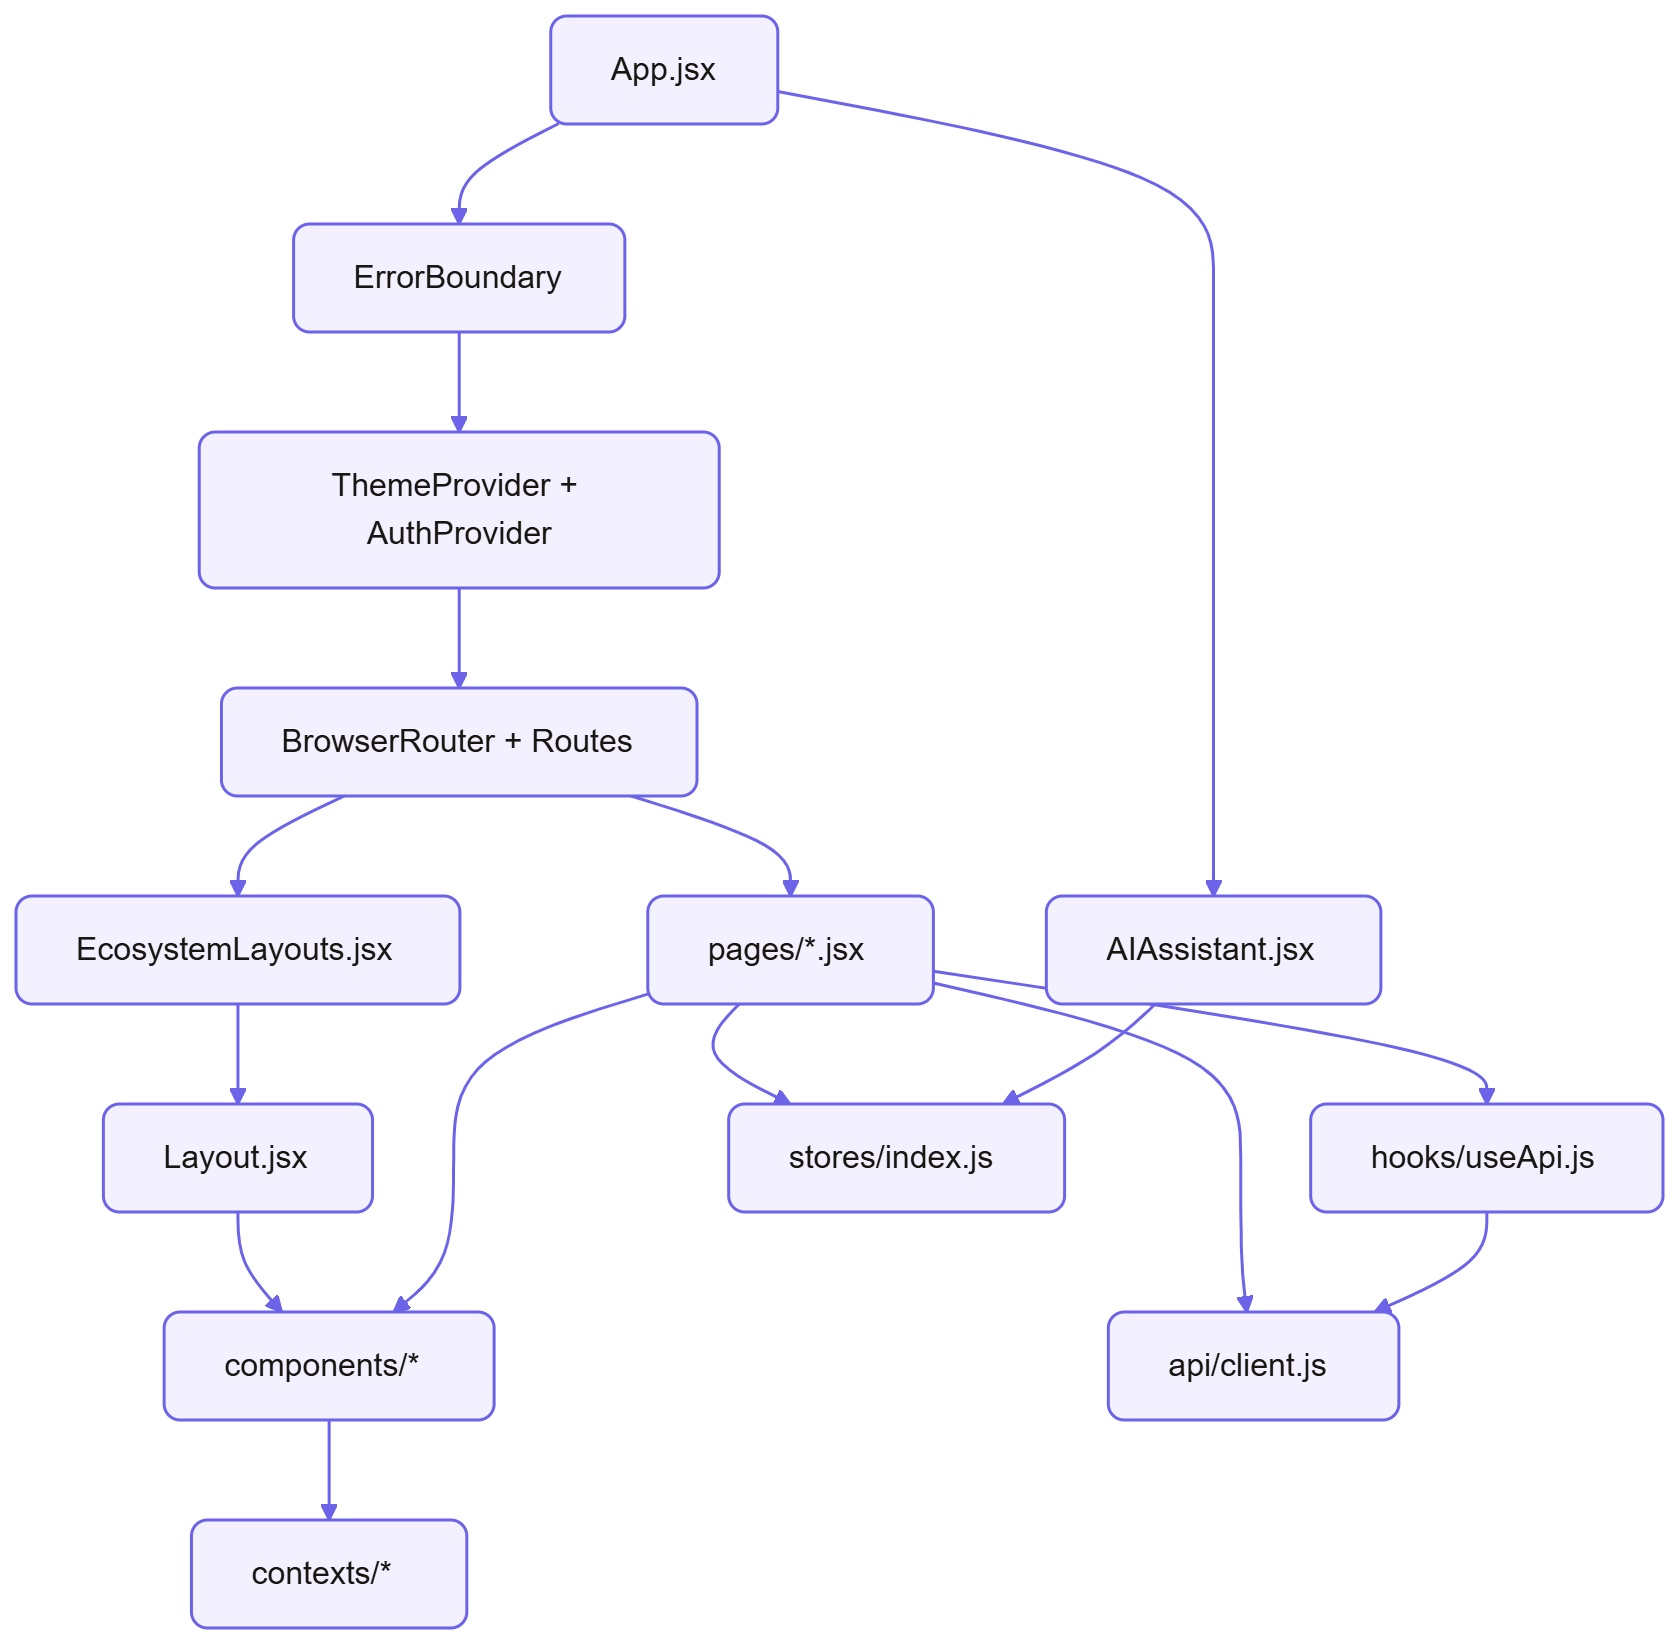
\includegraphics[width=0.7\textwidth]{Media/Chapter 4/2 React Component Architecture.jpg}
\caption{React Component Architecture of PrepSmart}
\label{fig:react_architecture}
\end{figure}

The React application is organized around a hierarchical component structure that separates application initialization, routing, layout management, reusable components, and API communication into independent modules.

The application execution begins from the App component, which acts as the entry point of the frontend application. The App component initializes the global providers, configures routing, and renders the major modules of the application.

Global state management is handled through the ThemeProvider and AuthProvider components. ThemeProvider maintains the application's appearance settings, including light and dark themes, while AuthProvider manages authentication state, user information, access tokens, and session persistence throughout the application.

Navigation within the application is implemented using BrowserRouter. Instead of loading separate HTML pages, BrowserRouter dynamically renders React components according to the current URL, thereby providing a seamless Single Page Application experience.

The Layout component provides a consistent user interface across different pages by managing the navigation bar, sidebar, footer, and common interface elements. Individual pages such as Dashboard, Learning Modules, Coding Practice, Interview Preparation, Company Readiness, Portfolio Management, and Profile Management are rendered within this layout.

Reusable UI components are organized separately from page-level components. These reusable components include cards, buttons, forms, charts, dialogs, tables, progress indicators, and visualization widgets that are shared across multiple pages, reducing code duplication and improving consistency.

Communication with the backend is centralized through the API Client module. Instead of making HTTP requests directly from individual pages, all API interactions are performed through a common client that automatically attaches authentication tokens, processes server responses, and handles error conditions consistently.

Application-wide state management is further supported through React Contexts and Stores. These modules maintain shared application data such as authentication status, dashboard information, user preferences, and placement preparation progress without requiring excessive component-to-component communication.

The frontend also integrates an AI Assistant component that provides intelligent assistance and interacts with backend AI services whenever supported functionality is available.

\subsection{Advantages of the Frontend Architecture}

The frontend architecture adopted in PrepSmart offers several advantages.

\begin{itemize}

\item Component-based development improves code reusability.

\item Single Page Application architecture provides faster navigation.

\item Centralized API communication simplifies backend integration.

\item Context Providers enable efficient global state management.

\item Reusable UI components improve maintainability.

\item Modular organization facilitates future feature expansion.

\item Dynamic rendering enhances user experience without full page reloads.

\end{itemize}

\section{Backend Implementation}

The backend of PrepSmart has been developed using Django and Django REST Framework (DRF), following a modular architecture that separates authentication, business logic, database operations, and API communication into independent components. The backend serves as the central processing unit of the platform by handling client requests, validating user permissions, executing application logic, interacting with the database, and generating structured JSON responses.

RESTful APIs are used as the communication mechanism between the React frontend and the Django backend. Each client request passes through authentication and validation before the corresponding business logic is executed. This architecture improves security, maintainability, and scalability while supporting efficient interaction between the frontend and backend.

Figure~\ref{fig:api_request_flow} illustrates the request processing workflow adopted in PrepSmart.

\begin{figure}[H]
\centering
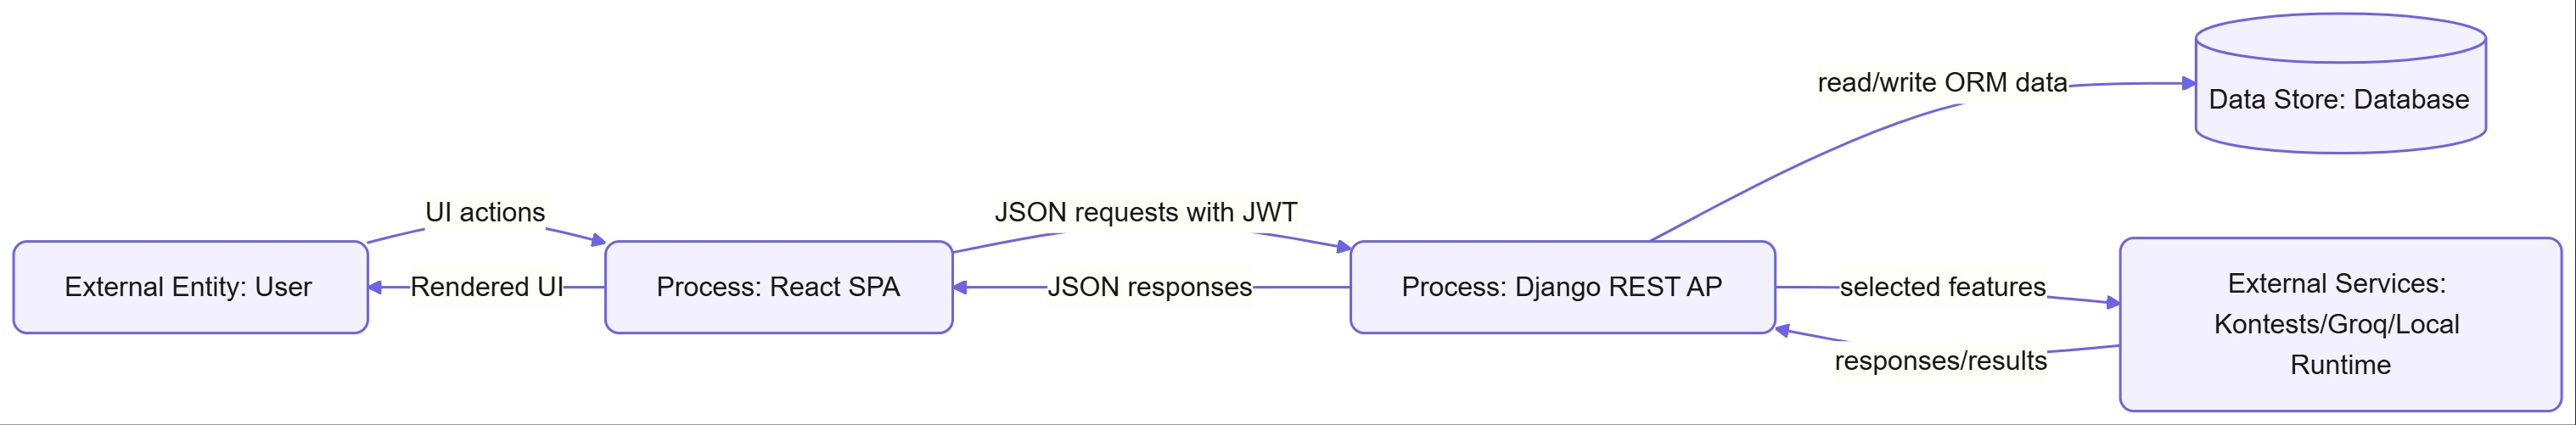
\includegraphics[width=\textwidth]{Media/Chapter 4/7 API Request Flow.jpg}
\caption{API Request Flow in PrepSmart}
\label{fig:api_request_flow}
\end{figure}

The API request processing begins when a user performs an action through the React frontend, such as logging into the system, starting a mock test, submitting code, or viewing dashboard statistics. The frontend sends an HTTP request through the centralized API Client using the appropriate REST endpoint.

The API Client automatically attaches the required HTTP headers, including the JSON Web Token (JWT) for authenticated requests. This ensures that protected resources are accessible only to authorized users.

The request is received by Django REST Framework, where authentication and permission checks are performed before forwarding the request to the appropriate API View. Each API View is responsible for processing a specific functionality of the platform, such as user authentication, topic management, coding practice, interview sessions, or dashboard analytics.

The API View interacts with Django ORM to retrieve or update application data stored in the relational database. Business rules, validation logic, and data processing are executed within the backend before generating the response.

Once processing is complete, the backend returns a structured JSON response containing the requested information or the execution result. The React frontend receives this response and dynamically updates the user interface without requiring a complete page refresh, thereby providing a responsive and seamless user experience.

\subsection{API Request Processing Workflow}

The request handling mechanism followed by PrepSmart consists of the following sequential steps:

\begin{enumerate}

\item The user performs an operation through the React web interface.

\item The API Client generates an HTTP request and attaches the necessary authentication headers.

\item Django REST Framework authenticates the request using JSON Web Tokens (JWT).

\item The request is forwarded to the corresponding API View.

\item The API View executes the required business logic.

\item Django ORM performs the required database operations.

\item The processed result is converted into a JSON response.

\item The frontend receives the response and updates the user interface dynamically.

\end{enumerate}

\subsection{Advantages of the Backend Architecture}

The backend implementation adopted in PrepSmart provides several advantages.

\begin{itemize}

\item Modular organization of backend services.

\item Secure RESTful communication using JWT authentication.

\item Efficient database interaction through Django ORM.

\item Separation of business logic from presentation logic.

\item Standardized JSON-based API communication.

\item Improved scalability through independent backend modules.

\item Easy integration with external APIs and AI services.

\end{itemize}

\section{Authentication Module}

Authentication is a fundamental component of the PrepSmart platform, ensuring that only authorized users can access protected resources and personalized placement preparation features. The system implements token-based authentication using JSON Web Tokens (JWT), providing a secure and scalable mechanism for user verification and session management.

The authentication module supports user registration, login, session validation, token refresh, and logout operations. Upon successful authentication, the backend generates an access token and a refresh token, which are securely managed by the frontend to maintain user sessions.

Figure~\ref{fig:authentication_sequence} illustrates the authentication workflow implemented in PrepSmart.

\begin{figure}[H]
\centering
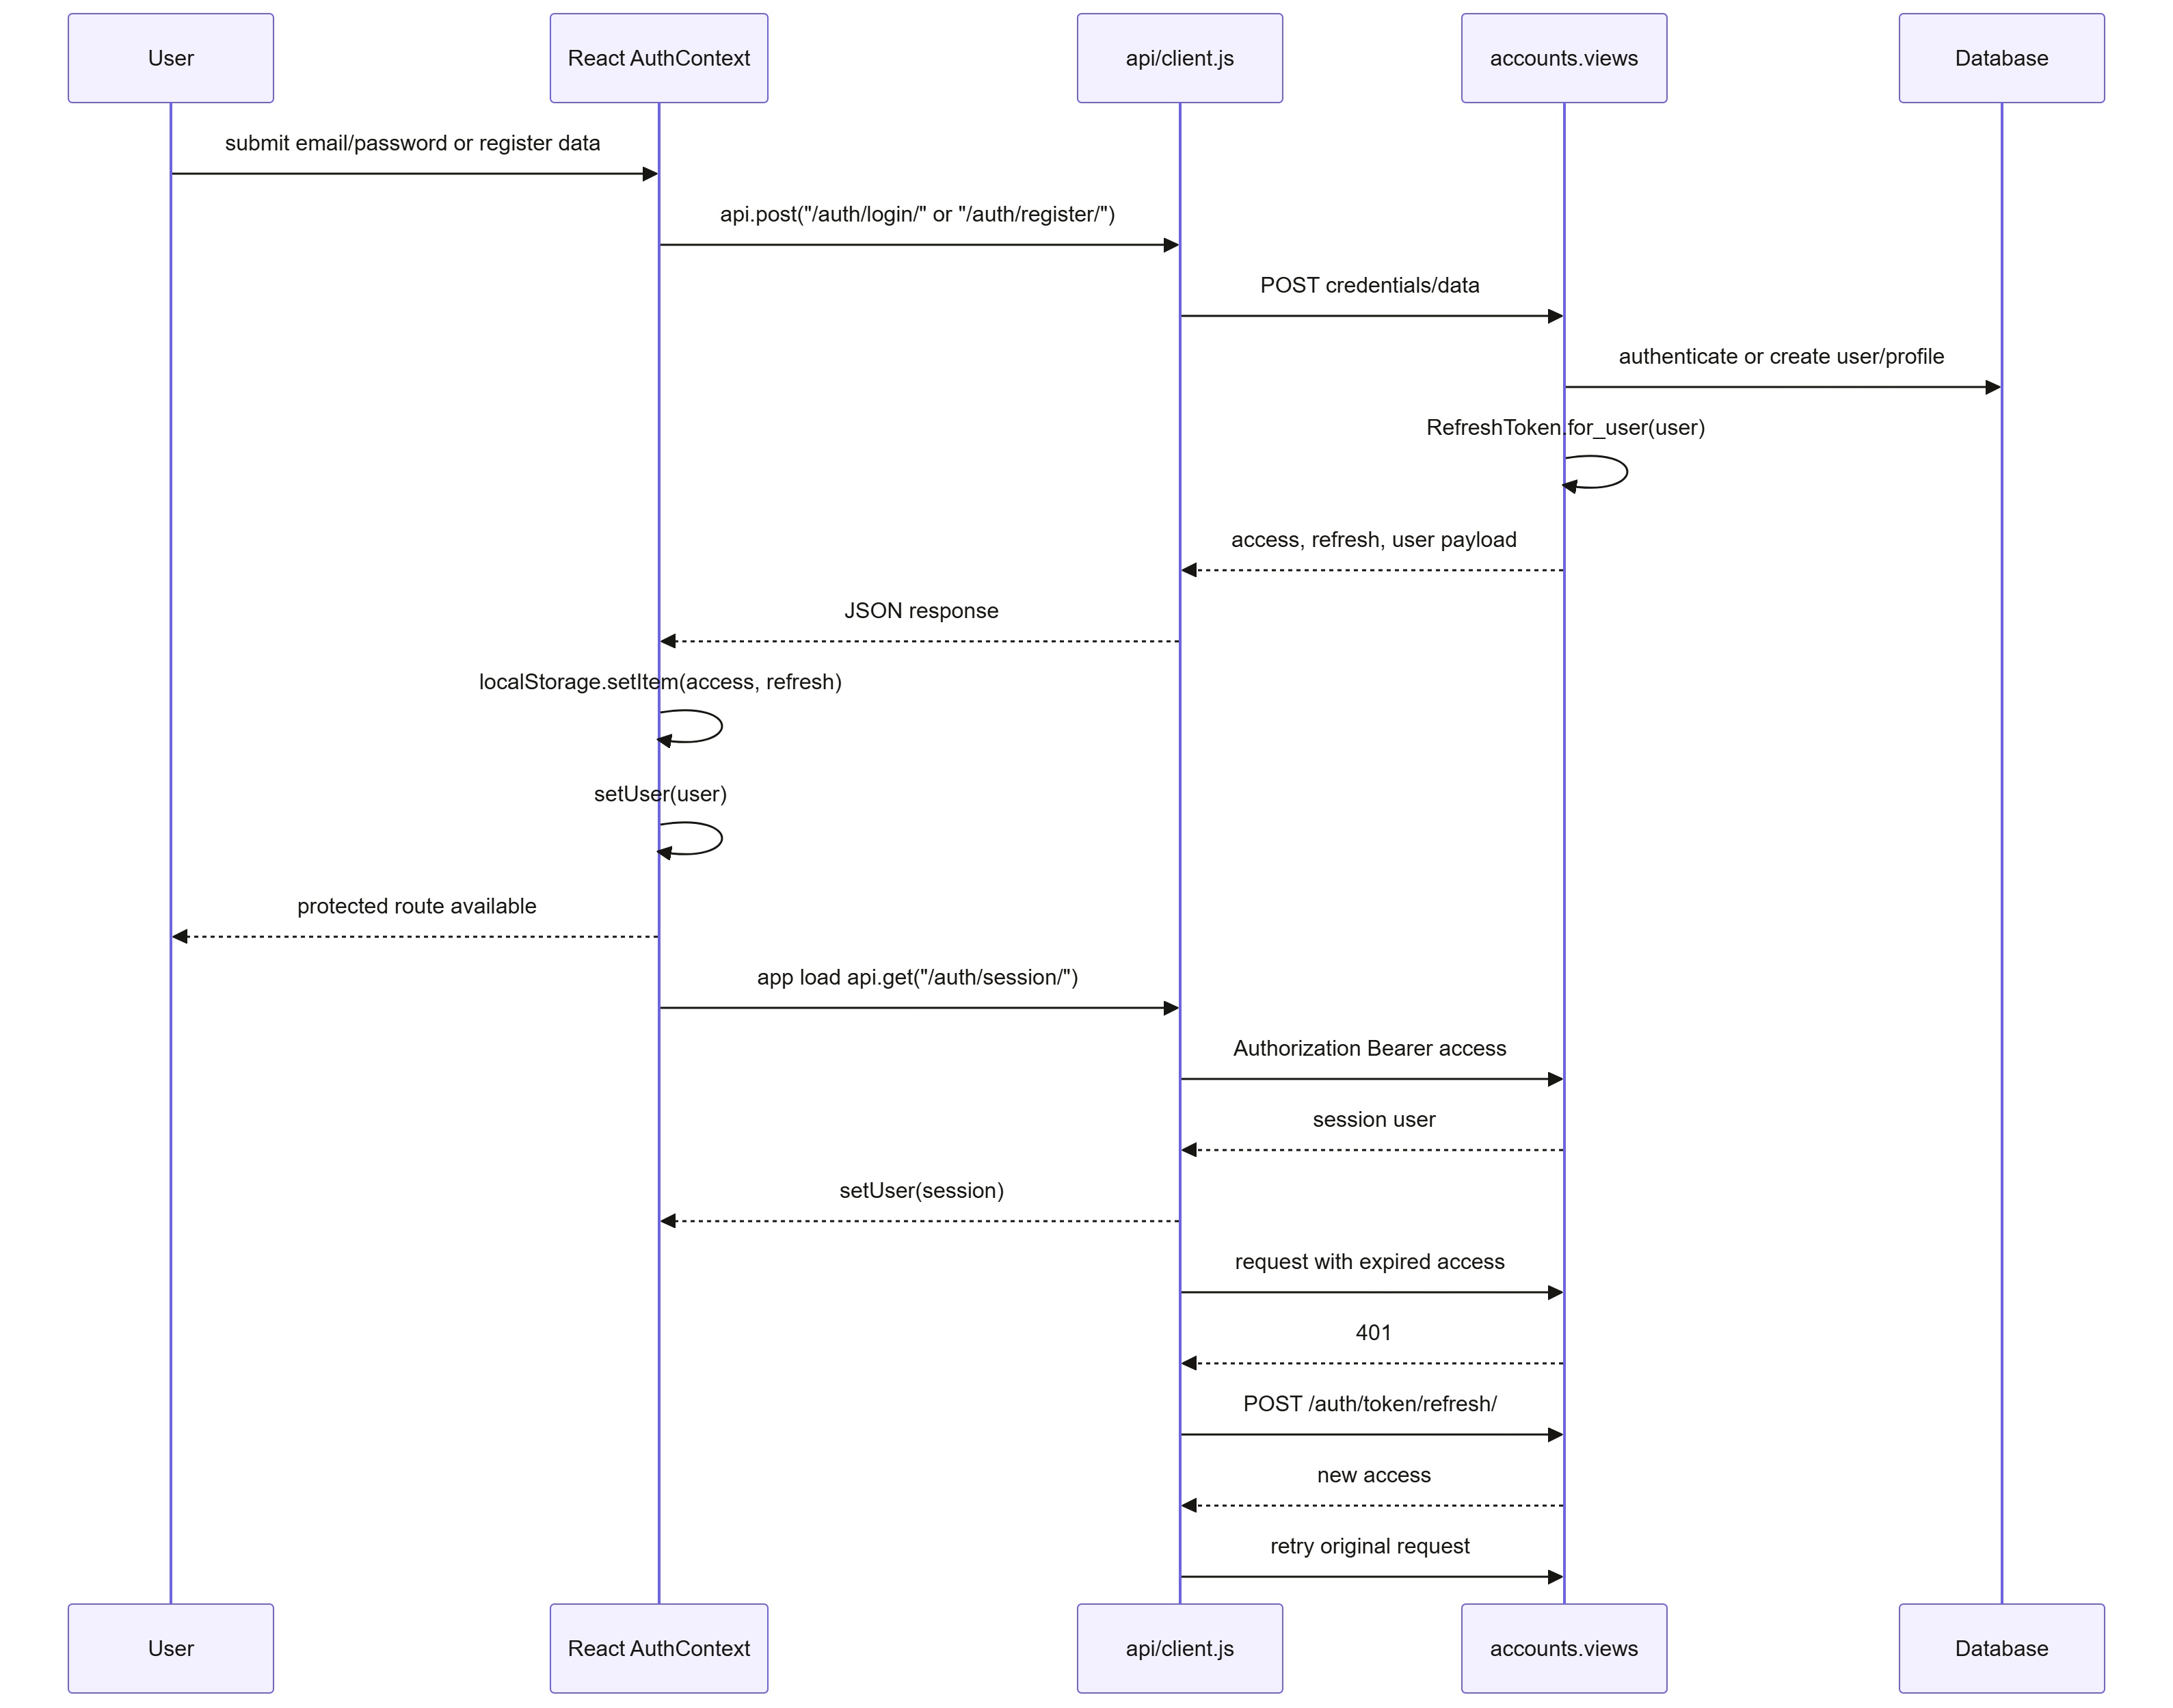
\includegraphics[width=0.83\textwidth]{Media/Chapter 4/9 Authentication Sequence.jpg}
\caption{Authentication Sequence Diagram of PrepSmart}
\label{fig:authentication_sequence}
\end{figure}

The authentication process begins when a user submits valid login credentials through the React frontend. The Auth Context forwards the credentials to the centralized API Client, which sends an authenticated HTTP POST request to the login endpoint exposed by Django REST Framework.

The backend verifies the supplied credentials against the stored user information in the database. If the credentials are valid, Django generates a JSON Web Token (JWT) pair consisting of an access token and a refresh token. Along with these tokens, the authenticated user's profile information is returned to the frontend.

The React application stores the received tokens securely in the browser's local storage and updates the authentication context with the logged-in user's information. Once authentication is successful, the user is redirected to the protected areas of the platform such as the dashboard, learning modules, coding workspace, and interview preparation pages.

Whenever the application starts, the frontend checks whether a valid user session already exists by requesting the session endpoint. If the access token is still valid, the backend returns the authenticated user's information and restores the session without requiring the user to log in again.

If an access token expires during API communication, the backend responds with an unauthorized status code. The API Client automatically sends the stored refresh token to the token refresh endpoint, receives a new access token, updates local storage, and retries the original request. This automatic refresh mechanism provides a seamless user experience while maintaining secure authentication throughout the application.

\subsection{Authentication Workflow}

The authentication mechanism implemented in PrepSmart follows the sequence below.

\begin{enumerate}

\item The user enters login credentials.

\item The frontend sends the credentials to the authentication API.

\item Django verifies the credentials using the user database.

\item A JWT access token and refresh token are generated.

\item Both tokens are returned to the frontend.

\item The frontend stores the tokens securely in local storage.

\item Protected API requests include the access token in the Authorization header.

\item If the access token expires, the refresh token is used to obtain a new access token.

\item The original API request is automatically retried without requiring the user to log in again.

\end{enumerate}

\subsection{Security Features}

The authentication module incorporates several security mechanisms to protect user accounts and application resources.

\begin{itemize}

\item Token-based authentication using JSON Web Tokens (JWT).

\item Secure separation of access tokens and refresh tokens.

\item Authentication of every protected API endpoint.

\item Automatic token refresh without interrupting the user session.

\item Prevention of unauthorized access through backend permission checks.

\item Session restoration after successful token validation.

\item Centralized authentication management using React Context.

\end{itemize}

\subsection{Advantages of the Authentication Module}

The implemented authentication mechanism provides several advantages.

\begin{itemize}

\item Secure user authentication.

\item Stateless communication between frontend and backend.

\item Reduced server-side session management.

\item Improved scalability for multiple concurrent users.

\item Seamless user experience through automatic token refresh.

\item Simplified integration with RESTful APIs.

\end{itemize}

\section{Placement Preparation Module}

The Placement Preparation Module forms the core functionality of the PrepSmart platform. It provides students with a structured learning journey that organizes placement preparation into tracks, topics, quizzes, coding exercises, and progress monitoring. The objective of this module is to guide students through a systematic learning process instead of relying on fragmented preparation across multiple platforms.

The module continuously records user activities, evaluates learning progress, and updates completion status after every learning activity. This enables students to monitor their preparation while allowing the system to generate personalized recommendations and readiness analytics.

Figure~\ref{fig:prep_journey} illustrates the workflow of the Placement Preparation Module.

\begin{figure}[H]
\centering
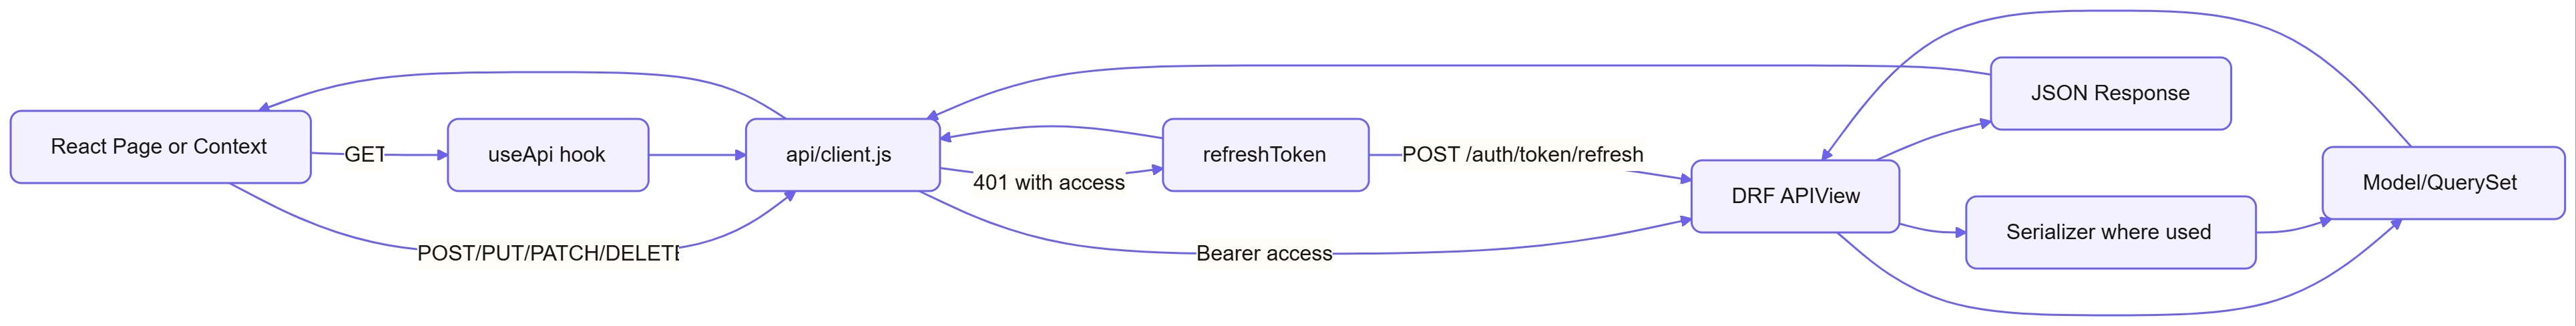
\includegraphics[width=\textwidth]{Media/Chapter 4/11 Preparation Journey Workflow.jpg}
\caption{Placement Preparation Workflow}
\label{fig:prep_journey}
\end{figure}

The placement preparation process begins when an authenticated student selects a learning track or topic from the frontend interface. The request is forwarded to the backend through the centralized API client, where the corresponding API endpoints process the request and retrieve the required learning content.

When a student completes a topic, the frontend sends a completion request to the backend. The backend verifies the authenticated user, retrieves the selected topic, and updates the corresponding learning progress record in the database. If the topic is being completed for the first time, the system creates a new progress entry and records the completion timestamp.

After completing the theoretical content, students attempt the topic quiz. Quiz responses are submitted to the backend, where each answer is evaluated against the stored correct answers. The backend calculates the student's accuracy and stores the result in the database. If the obtained score satisfies the predefined completion criteria, the corresponding topic is automatically marked as completed.

Every completed learning activity is recorded as an activity event, allowing the dashboard and analytics module to generate progress reports, calculate completion percentages, and recommend subsequent learning topics. This automated workflow ensures that students follow a structured placement preparation path while continuously tracking their overall readiness.

\subsection{Placement Preparation Workflow}

The Placement Preparation Module follows the workflow below.

\begin{enumerate}

\item The student selects a learning track.

\item The frontend requests the corresponding learning topics.

\item The backend retrieves topic information from the database.

\item The student studies the selected topic.

\item The student marks the topic as completed.

\item The backend updates the UserTopicProgress table.

\item The student attempts the topic quiz.

\item The backend evaluates quiz responses.

\item Progress statistics are updated.

\item Dashboard analytics are refreshed automatically.

\end{enumerate}

\subsection{Major Features}

The Placement Preparation Module provides the following features.

\begin{itemize}

\item Structured learning tracks.

\item Topic-wise study materials.

\item Quiz-based assessment.

\item Automatic progress tracking.

\item Activity logging.

\item Personalized learning journey.

\item Readiness score calculation.

\item Integration with dashboard analytics.

\end{itemize}

\subsection{Advantages of the Placement Preparation Module}

The implemented module offers several advantages.

\begin{itemize}

\item Organizes placement preparation into structured learning paths.

\item Eliminates fragmented learning across multiple platforms.

\item Automatically tracks student progress.

\item Provides continuous assessment through quizzes.

\item Enables personalized learning recommendations.

\item Supports future expansion with additional learning tracks.

\end{itemize}

\section{Dashboard and Analytics Module}

The Dashboard and Analytics Module provides students with a centralized view of their placement preparation progress. It aggregates learning activities, coding practice, quiz performance, interview readiness, company preparation, and daily goals into a single interactive dashboard. This enables students to monitor their overall progress and identify areas requiring improvement.

Figure~\ref{fig:dashboard_workflow} illustrates the workflow of the Dashboard and Analytics Module.

\begin{figure}[H]
\centering
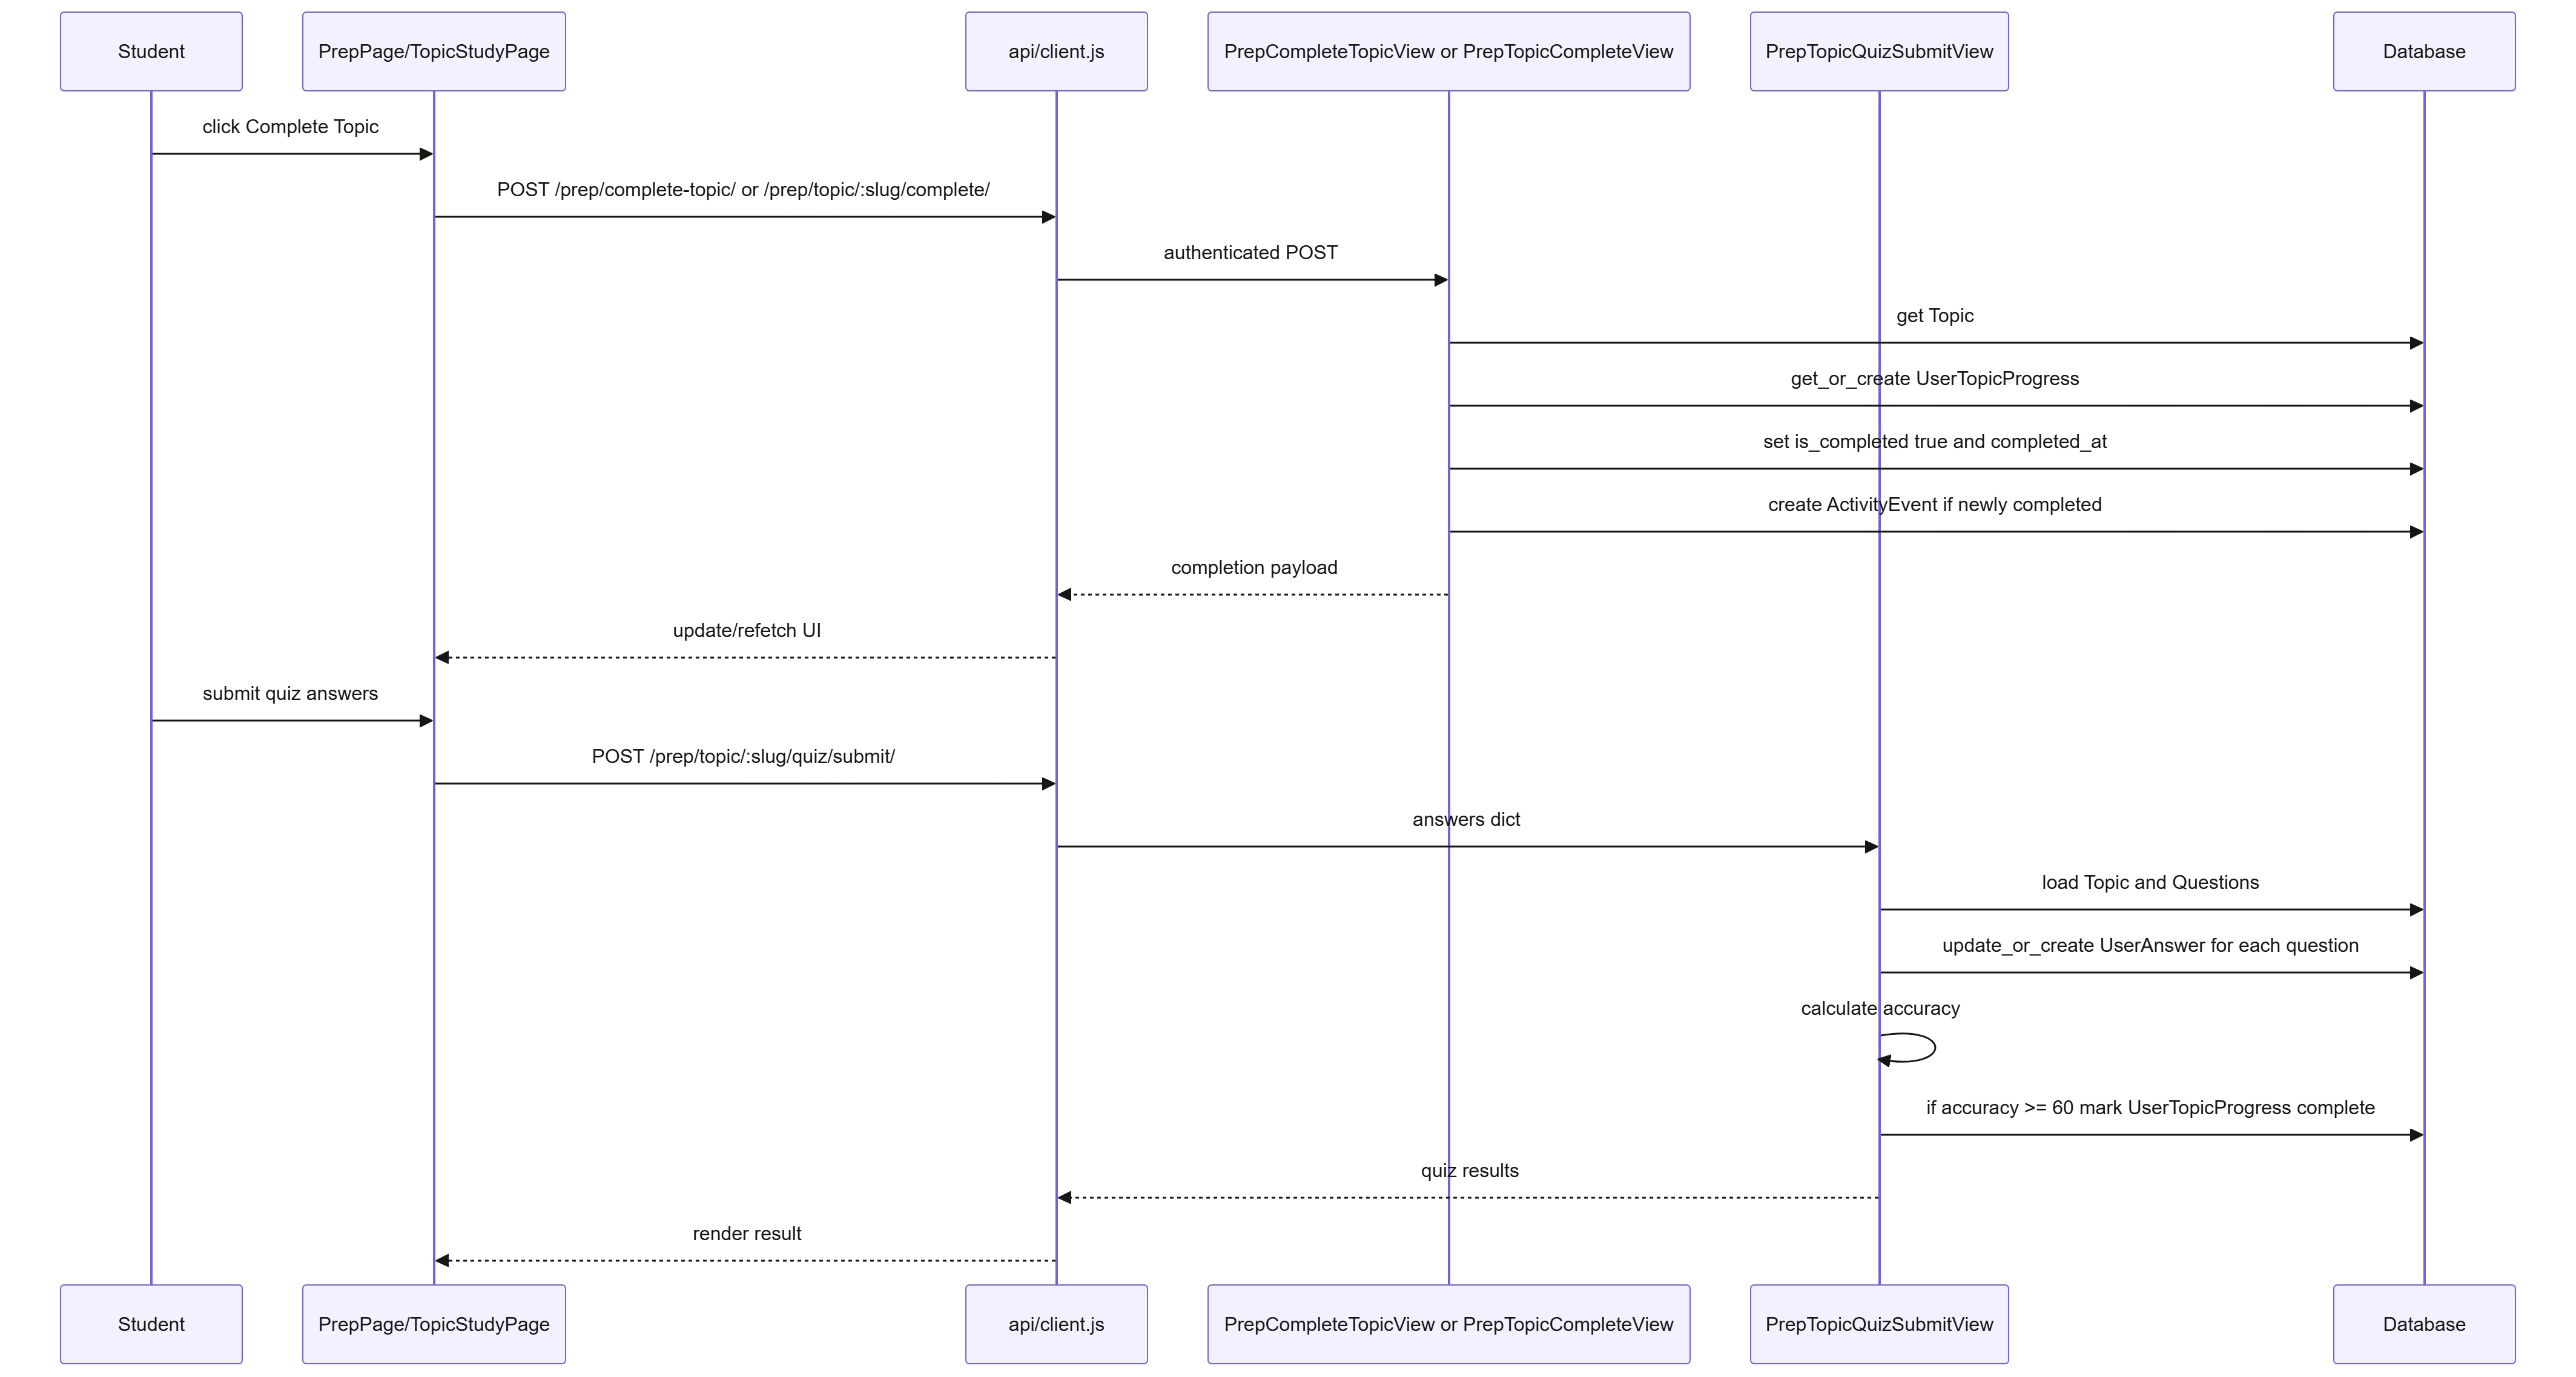
\includegraphics[width=\textwidth]{Media/Chapter 4/12 Dashboard Workflow.jpg}
\caption{Dashboard and Analytics Workflow}
\label{fig:dashboard_workflow}
\end{figure}

The dashboard is generated dynamically whenever an authenticated user accesses the application. The frontend requests dashboard information through the Dashboard API, which collects data from multiple backend modules.

The backend retrieves information related to user profiles, completed topics, quiz attempts, coding submissions, interview sessions, daily goals, revision schedules, company readiness records, and activity history. These records are processed to calculate important performance indicators such as completion percentage, quiz accuracy, coding statistics, interview readiness score, daily learning streak, and overall placement readiness.

The processed data is returned to the frontend as structured JSON responses. The React application visualizes this information using charts, progress indicators, summary cards, and statistical widgets. Since the dashboard retrieves live information from the database, users always receive updated analytics reflecting their latest activities.

The dashboard also serves as a personalized learning assistant by highlighting pending topics, revision requirements, upcoming milestones, and company-specific preparation status. This enables students to make informed decisions regarding their preparation strategy.

\subsection{Dashboard Features}

The Dashboard and Analytics Module provides the following features.

\begin{itemize}

\item Overall placement readiness score.

\item Topic-wise completion statistics.

\item Coding practice performance.

\item Quiz and mock test analysis.

\item Interview readiness tracking.

\item Company preparation progress.

\item Daily learning goals and streak monitoring.

\item Activity history and recent achievements.

\item Personalized learning recommendations.

\end{itemize}

\subsection{Advantages of the Dashboard Module}

The dashboard implementation offers several advantages.

\begin{itemize}

\item Centralized visualization of student progress.

\item Real-time performance analytics.

\item Continuous monitoring of placement readiness.

\item Easy identification of weak topics.

\item Motivation through progress tracking and learning streaks.

\item Integration of multiple learning modules into a unified analytical interface.

\end{itemize}

\section{Mock Test Module}

The Mock Test Module enables students to evaluate their preparation by attempting topic-wise assessments and milestone-based mock examinations. The module simulates actual placement examinations by providing timed tests, automatic evaluation, score calculation, and performance analysis.

The objective of this module is to help students identify weak areas, improve problem-solving speed, and continuously monitor their placement readiness through regular assessments.

Figure~\ref{fig:mock_test_workflow} illustrates the workflow of the Mock Test Module.

\begin{figure}[H]
\centering
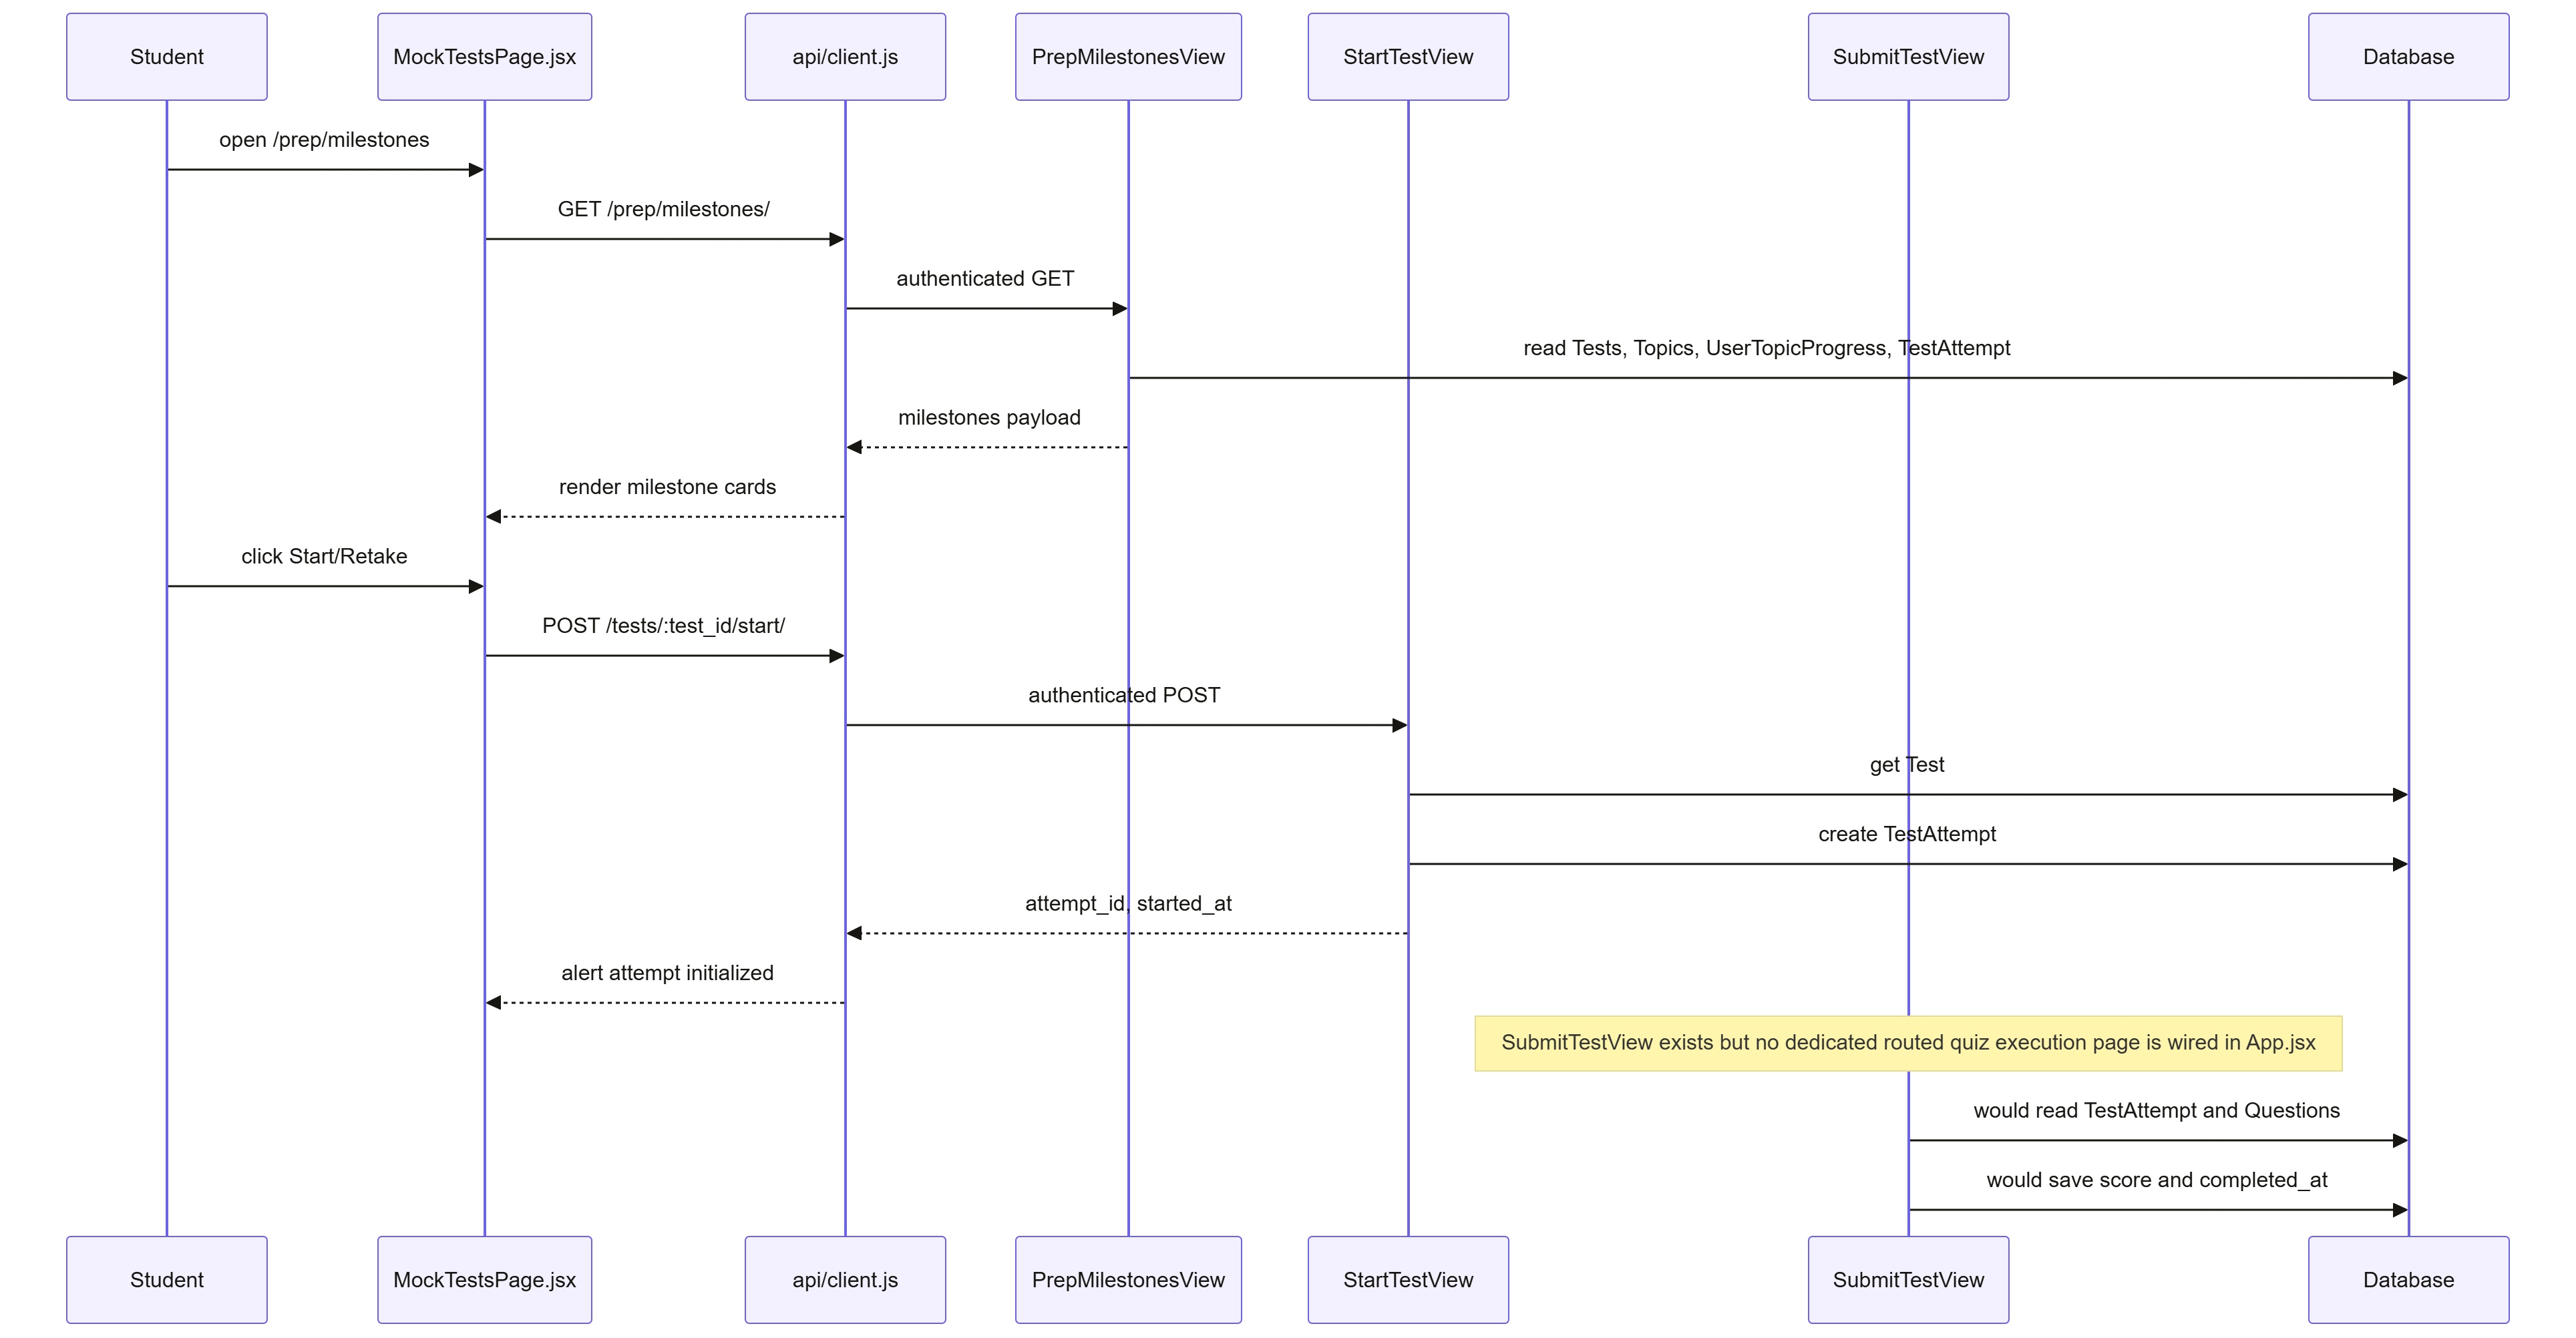
\includegraphics[width=\textwidth]{Media/Chapter 4/14 Mock Test Workflow.jpg}
\caption{Mock Test Workflow}
\label{fig:mock_test_workflow}
\end{figure}

The mock test process begins when an authenticated student selects a test from the available assessments displayed on the frontend. The React application requests the corresponding test details from the backend through the REST API.

The backend retrieves the selected test, associated topics, and question set from the database before creating a new TestAttempt record. This record stores the test identifier, start time, and user information, allowing the platform to track the student's progress throughout the assessment.

During the examination, students submit their answers through the frontend interface. The submitted responses are transmitted to the backend, where each answer is compared with the correct option stored in the database. The backend automatically calculates the obtained score, accuracy percentage, and other performance metrics before updating the TestAttempt record.

After evaluation, the calculated results are returned to the frontend and presented through scorecards, performance summaries, and topic-wise analysis. These results are also incorporated into the dashboard analytics module, enabling students to monitor their improvement over time and identify topics requiring additional practice.

\subsection{Mock Test Workflow}

The Mock Test Module follows the sequence below.

\begin{enumerate}

\item The student selects a mock test.

\item The frontend requests the test details.

\item The backend retrieves questions from the database.

\item A new TestAttempt record is created.

\item The student submits answers.

\item The backend evaluates each response.

\item The final score and statistics are calculated.

\item Results are stored in the database.

\item Performance analytics are updated.

\item The frontend displays the scorecard and analysis.

\end{enumerate}

\subsection{Major Features}

The Mock Test Module provides the following features.

\begin{itemize}

\item Topic-wise assessments.

\item Timed examinations.

\item Automatic evaluation.

\item Instant score generation.

\item Accuracy calculation.

\item Performance history.

\item Dashboard integration.

\item Continuous placement readiness assessment.

\end{itemize}

\subsection{Advantages of the Mock Test Module}

The implemented module provides several benefits.

\begin{itemize}

\item Simulates real placement examinations.

\item Provides immediate performance feedback.

\item Identifies weak learning areas.

\item Improves examination confidence.

\item Enables continuous progress tracking.

\item Supports data-driven preparation strategies.

\end{itemize}

\section{AI Interview Module}

The AI Interview Module is designed to simulate technical interview sessions and help students improve their communication, problem-solving, and technical knowledge. Unlike traditional question banks, this module provides an interactive interview experience by presenting questions, collecting responses, evaluating answers, and generating intelligent feedback using Artificial Intelligence.

The module supports different interview categories and maintains complete interview history, enabling students to monitor their progress over multiple interview sessions.

Figure~\ref{fig:ai_interview_workflow} illustrates the workflow of the AI Interview Module.

\begin{figure}[H]
\centering
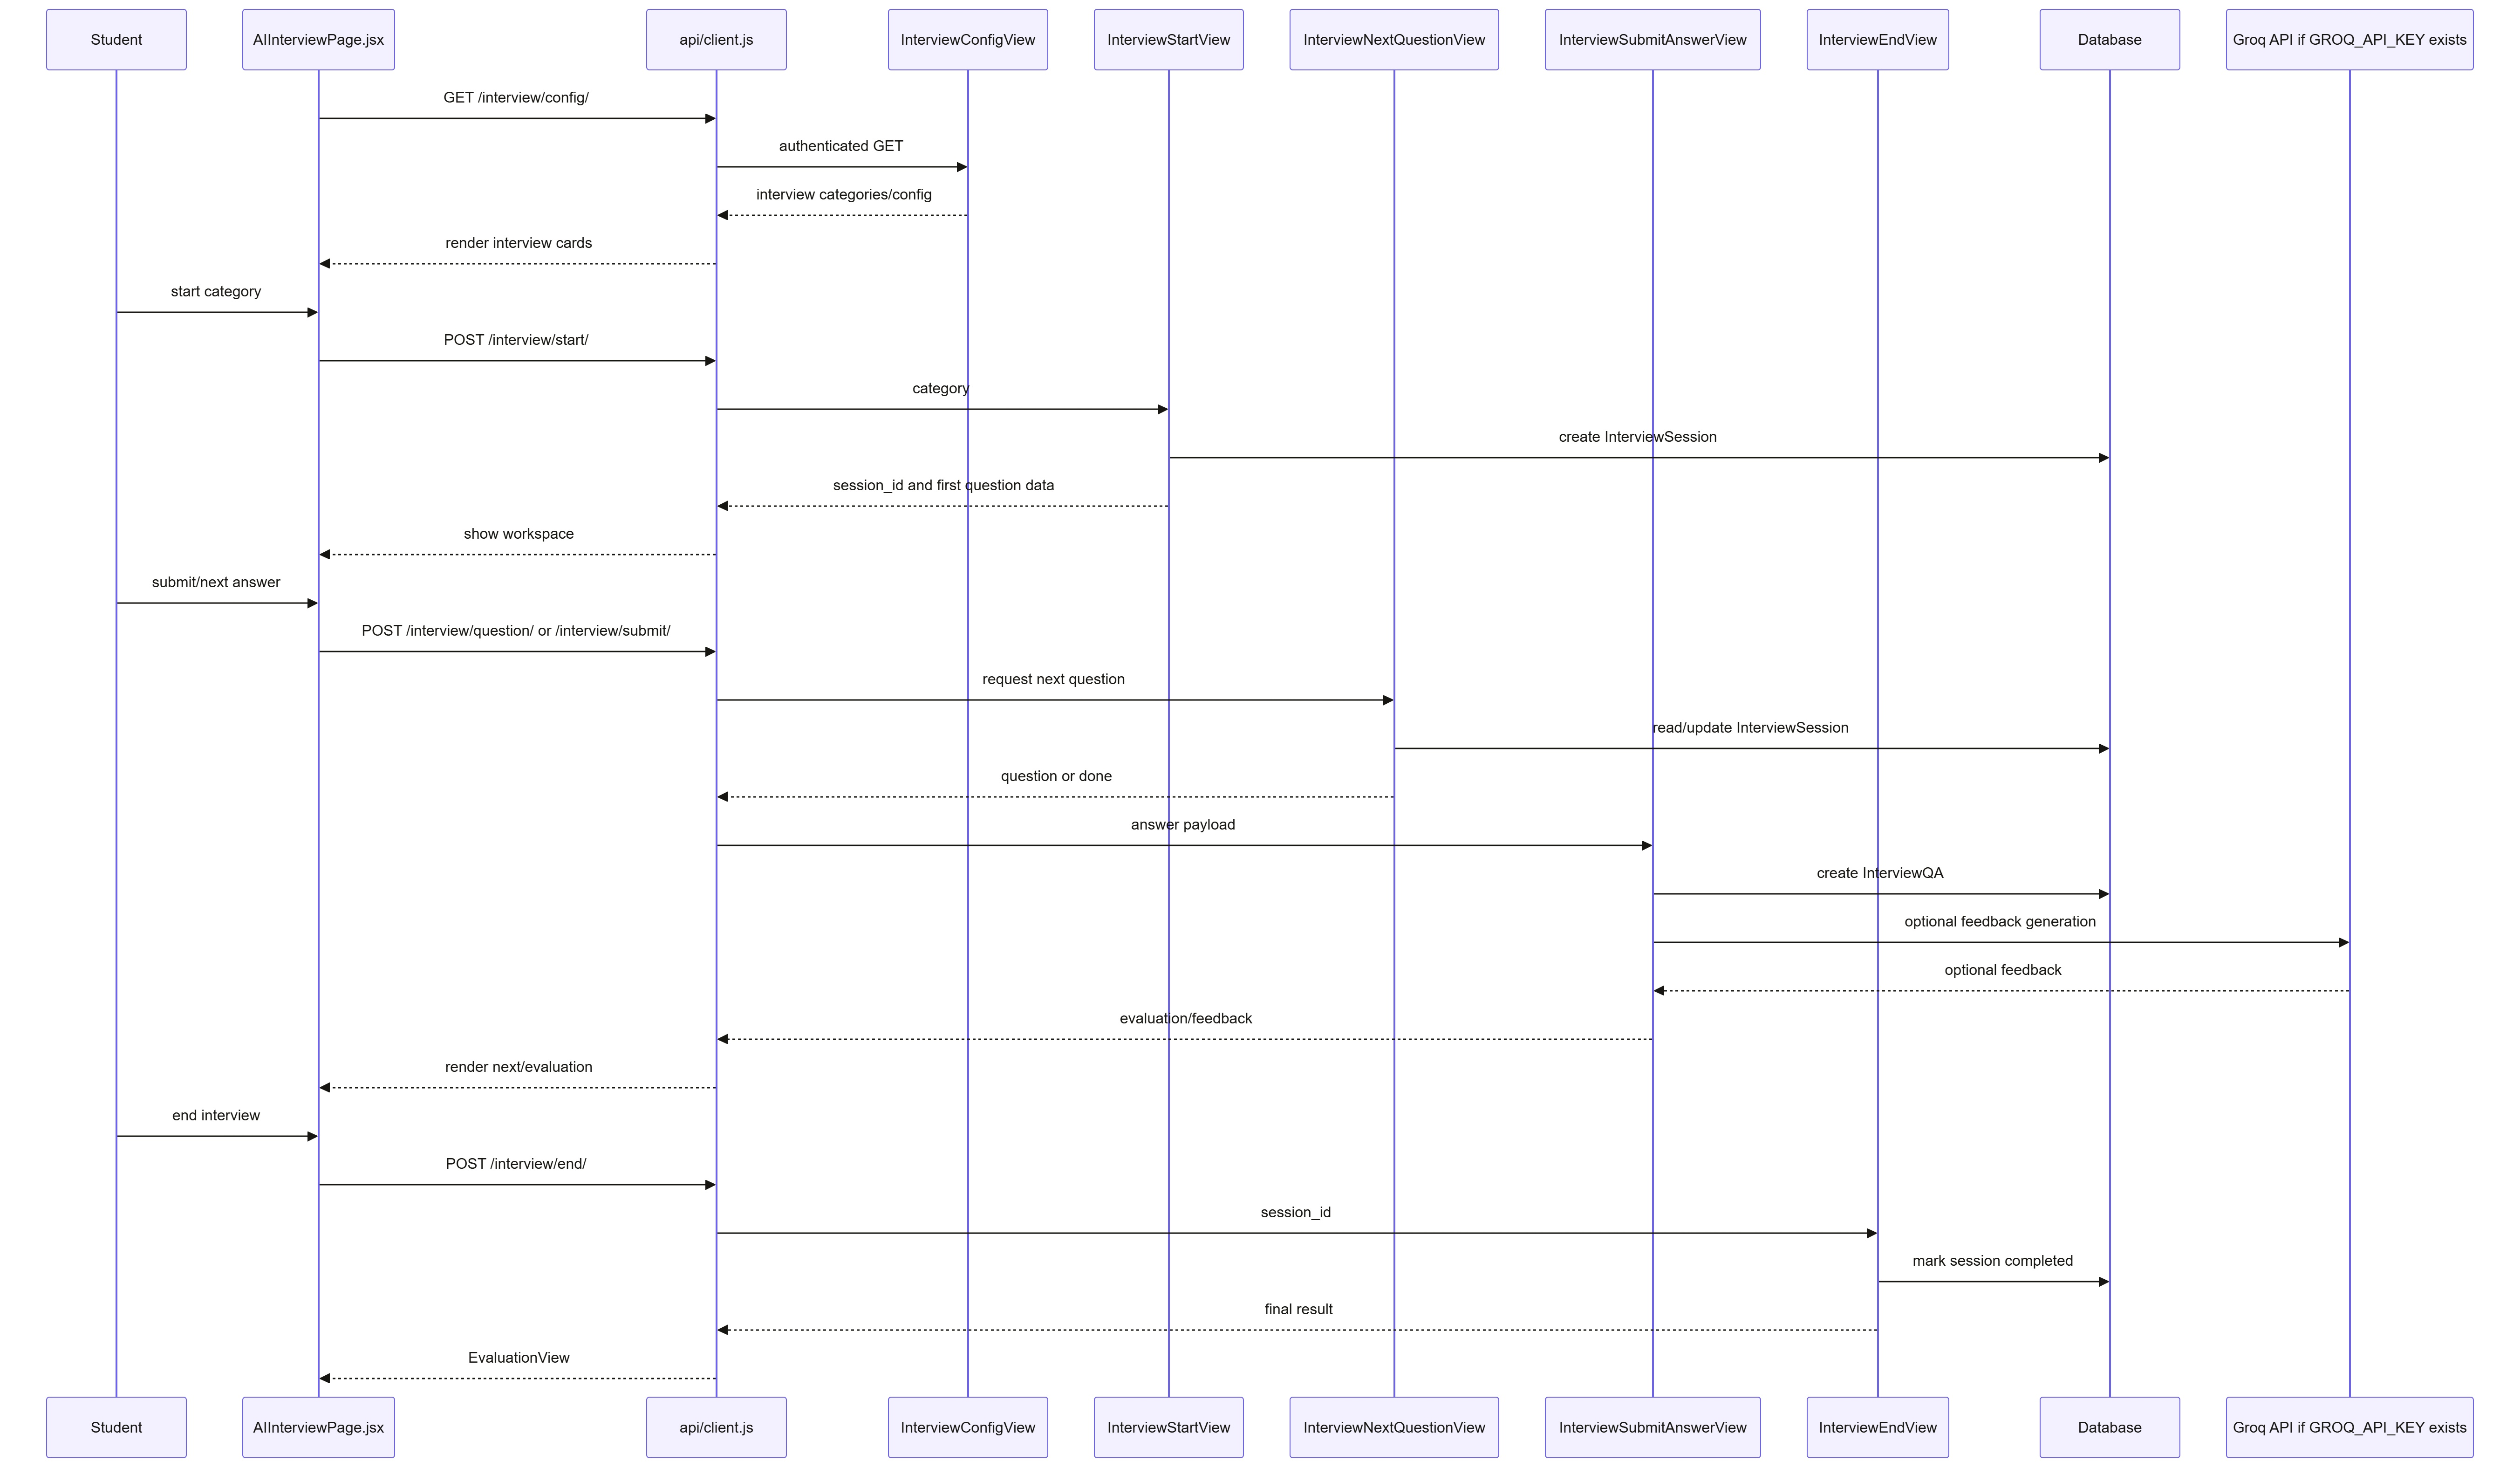
\includegraphics[width=\textwidth]{Media/Chapter 4/15 AI Interview Workflow.jpg}
\caption{AI Interview Workflow}
\label{fig:ai_interview_workflow}
\end{figure}

The AI Interview Module begins when an authenticated student selects an interview category through the frontend interface. The React application requests the available interview configuration from the backend, including interview categories and question settings.

After the interview configuration is loaded, the student starts a new interview session. The backend creates an InterviewSession record in the database and returns the first interview question to the frontend. Throughout the interview, each submitted response is transmitted to the backend for processing and evaluation.

The backend records every question and corresponding user response in the InterviewQA table. When AI functionality is enabled, the submitted answer is forwarded to the Groq API, which generates feedback regarding correctness, communication quality, technical depth, and possible improvements.

The generated feedback is returned to the frontend and displayed immediately after each response or at the end of the interview session, depending on the interview configuration. The backend also calculates interview scores and stores the final interview result, allowing students to review previous interview sessions and monitor their overall interview readiness.

\subsection{AI Interview Workflow}

The AI Interview Module follows the sequence below.

\begin{enumerate}

\item The student selects an interview category.

\item The frontend requests interview configuration.

\item The backend creates a new InterviewSession.

\item The first interview question is displayed.

\item The student submits an answer.

\item The backend records the response.

\item The answer is evaluated using backend logic and AI services.

\item Feedback and evaluation scores are generated.

\item The interview continues until all questions are completed.

\item The final interview report is stored and displayed.

\end{enumerate}

\subsection{Major Features}

The AI Interview Module provides the following features.

\begin{itemize}

\item Category-based interview sessions.

\item AI-assisted answer evaluation.

\item Automated interview scoring.

\item Detailed feedback generation.

\item Interview history management.

\item Readiness assessment.

\item Backend integration using REST APIs.

\item Secure storage of interview records.

\end{itemize}

\subsection{Advantages of the AI Interview Module}

The AI Interview Module offers several advantages.

\begin{itemize}

\item Simulates real technical interview experiences.

\item Provides immediate AI-generated feedback.

\item Improves communication and technical skills.

\item Enables continuous interview practice.

\item Tracks interview performance over time.

\item Supports personalized placement preparation.

\end{itemize}

\section{Coding Practice Module}

The Coding Practice Module enables students to solve programming problems directly within the PrepSmart platform. It provides an integrated coding environment where users can write, execute, and submit solutions without relying on external programming websites. The module supports multiple programming languages, automatic code evaluation, execution statistics, and result visualization.

The primary objective of this module is to strengthen problem-solving skills by providing an environment similar to technical coding interviews and online programming assessments.

Figure~\ref{fig:coding_workflow} illustrates the workflow of the Coding Practice Module.

\begin{figure}[H]
\centering
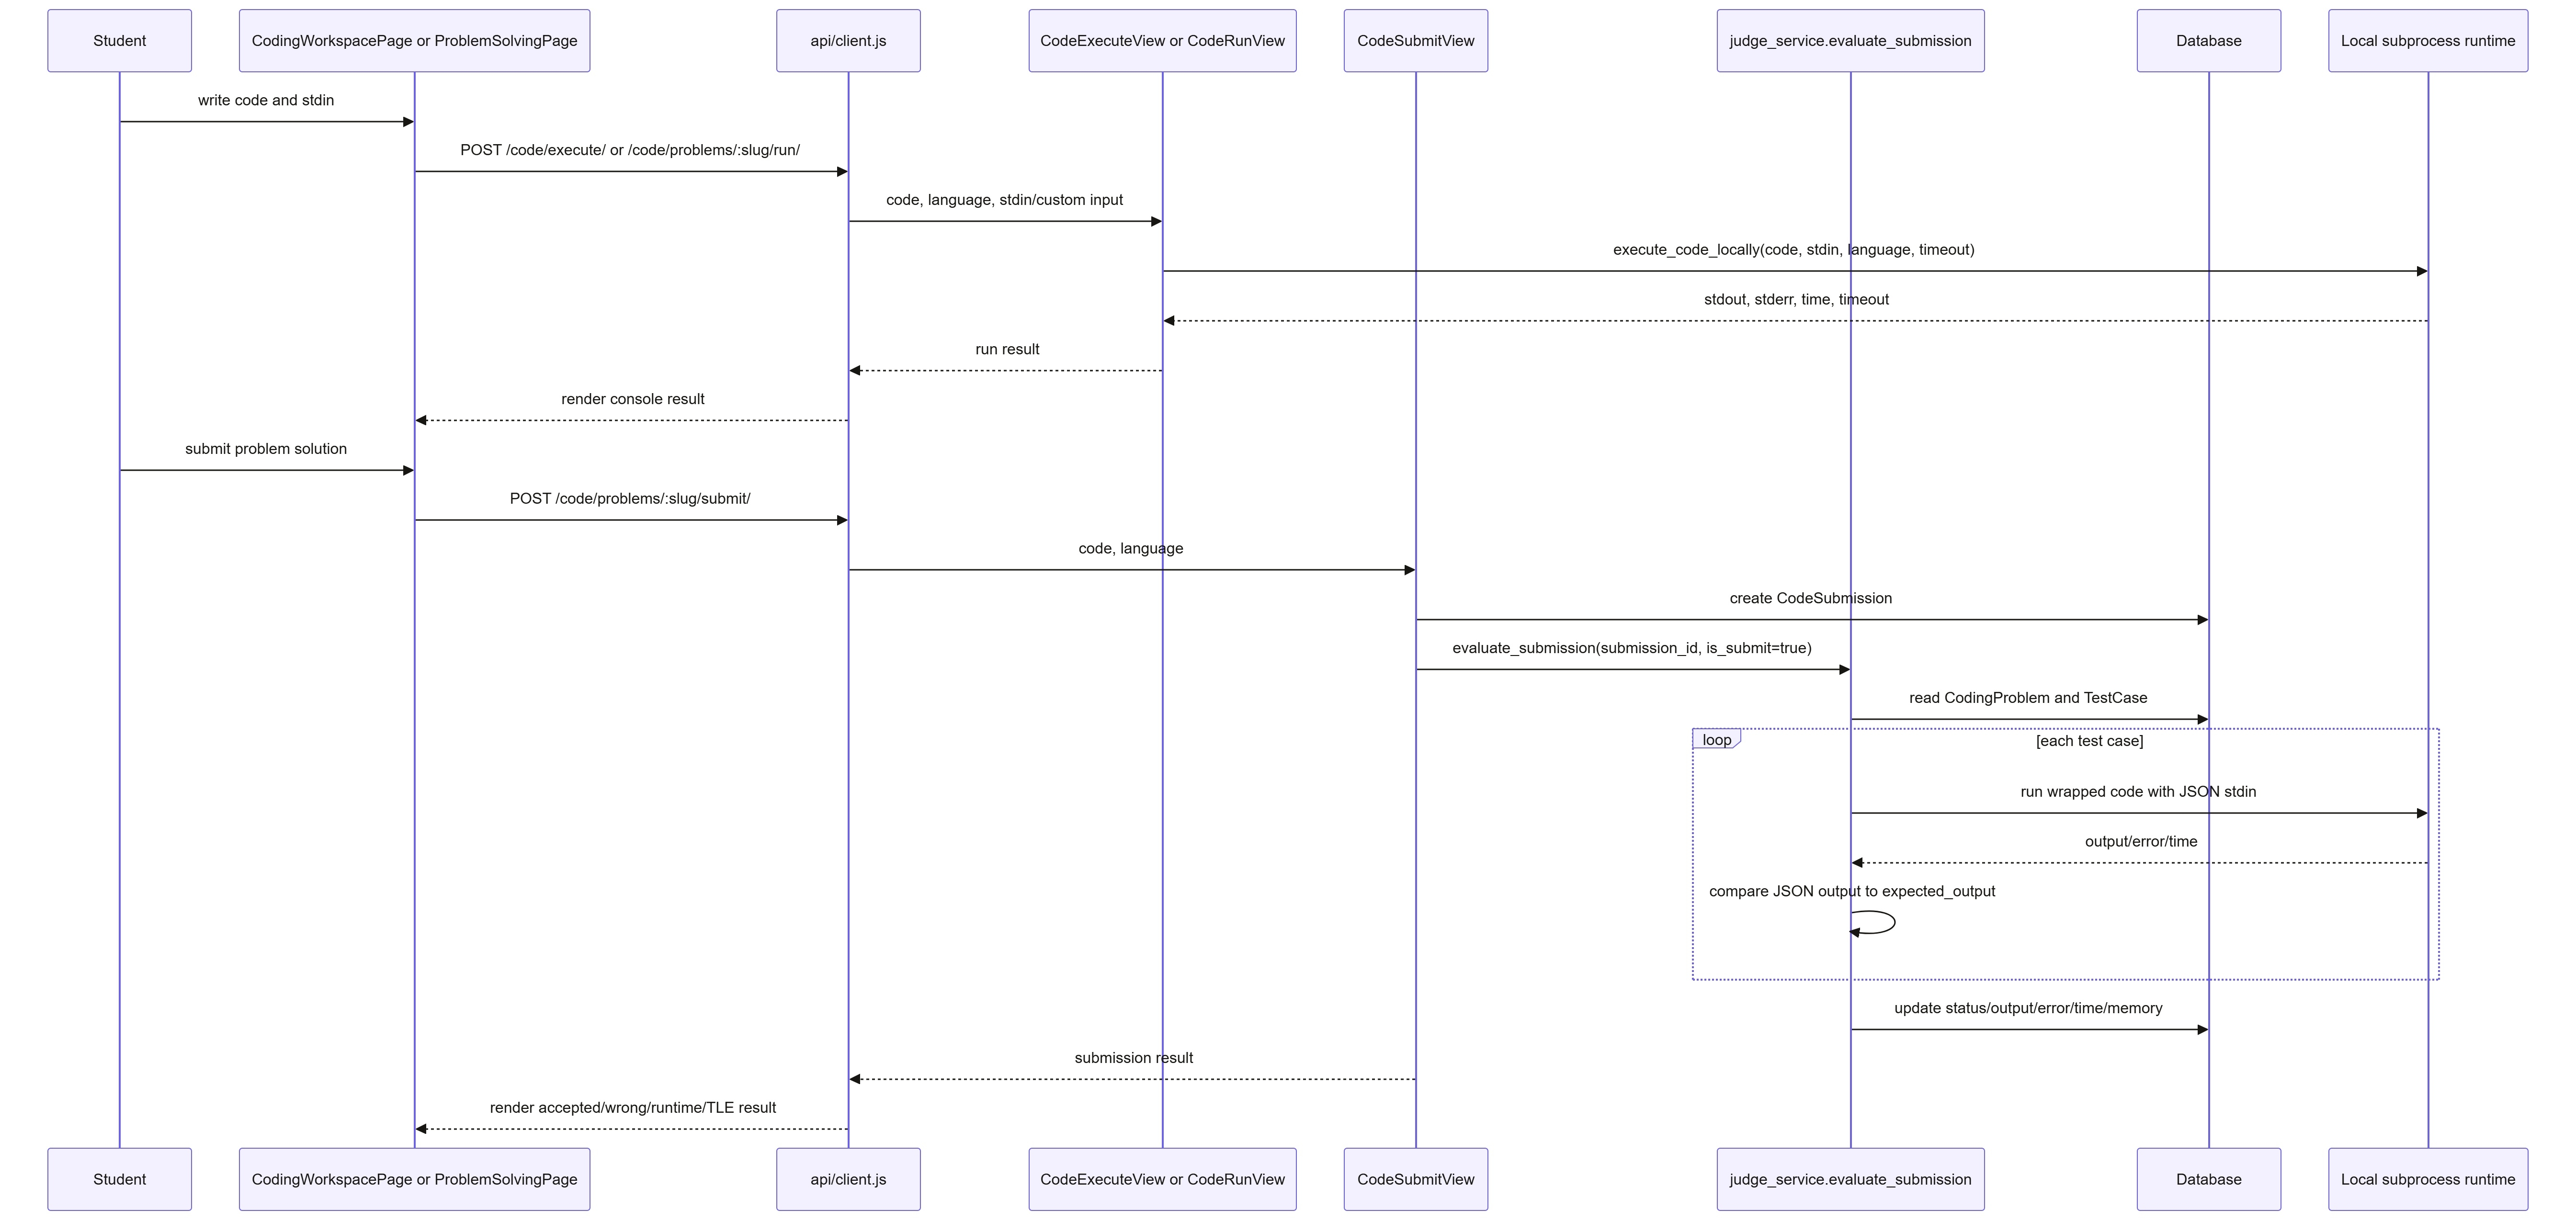
\includegraphics[width=\textwidth]{Media/Chapter 4/16 Coding Execution Workflow.jpg}
\caption{Coding Practice Workflow}
\label{fig:coding_workflow}
\end{figure}

The coding workflow begins when an authenticated student selects a programming problem from the coding workspace. The frontend retrieves the problem statement, constraints, supported programming languages, and starter code from the backend through REST APIs.

The student writes the solution using the integrated code editor and may execute the program using custom input before final submission. For execution requests, the frontend sends the source code, selected programming language, and input data to the backend.

The backend forwards the request to the local code execution engine, which compiles and executes the submitted program inside a controlled subprocess environment. During execution, the system records standard output, error messages, execution time, memory usage, and timeout status.

When the student submits the solution, a new CodeSubmission record is created in the database. The backend invokes the evaluation service, which executes the submitted program against all predefined test cases associated with the selected coding problem. The generated output is compared with the expected output for every test case to determine whether the solution is accepted.

After evaluation, the backend updates the submission status, execution statistics, runtime information, and evaluation result before returning the complete report to the frontend. The React application displays the evaluation outcome, enabling students to analyze errors, improve their solutions, and continue practicing programming problems.

\subsection{Coding Practice Workflow}

The Coding Practice Module follows the sequence below.

\begin{enumerate}

\item The student selects a programming problem.

\item The frontend retrieves the problem details.

\item The student writes source code using the integrated editor.

\item The code is executed using custom input when required.

\item The backend compiles and executes the program.

\item Execution statistics are collected.

\item The student submits the final solution.

\item The backend evaluates the solution against all test cases.

\item Submission results are stored in the database.

\item The frontend displays the final evaluation report.

\end{enumerate}

\subsection{Major Features}

The Coding Practice Module provides the following features.

\begin{itemize}

\item Integrated online code editor.

\item Support for multiple programming languages.

\item Custom input execution.

\item Automatic compilation and execution.

\item Test case based evaluation.

\item Runtime and memory analysis.

\item Submission history.

\item Secure local code execution environment.

\end{itemize}

\subsection{Advantages of the Coding Practice Module}

The Coding Practice Module provides several advantages.

\begin{itemize}

\item Provides an interview-like programming environment.

\item Enables immediate execution and evaluation of solutions.

\item Helps students improve coding efficiency.

\item Supports continuous programming practice.

\item Automatically records submission history.

\item Integrates coding performance with dashboard analytics.

\end{itemize}

\section{Portfolio and Skills Passport Module}

The Portfolio and Skills Passport Module enables students to build a professional digital profile that showcases their academic achievements, technical skills, projects, certifications, and overall placement readiness. Unlike traditional resumes, the module dynamically generates a structured portfolio and an employability passport using information already available within the PrepSmart platform.

The module also supports public sharing of portfolios through unique URLs, allowing recruiters and placement coordinators to review student profiles without requiring access to the internal system.

Figure~\ref{fig:portfolio_workflow} illustrates the workflow of the Portfolio and Skills Passport Module.

\begin{figure}[H]
\centering
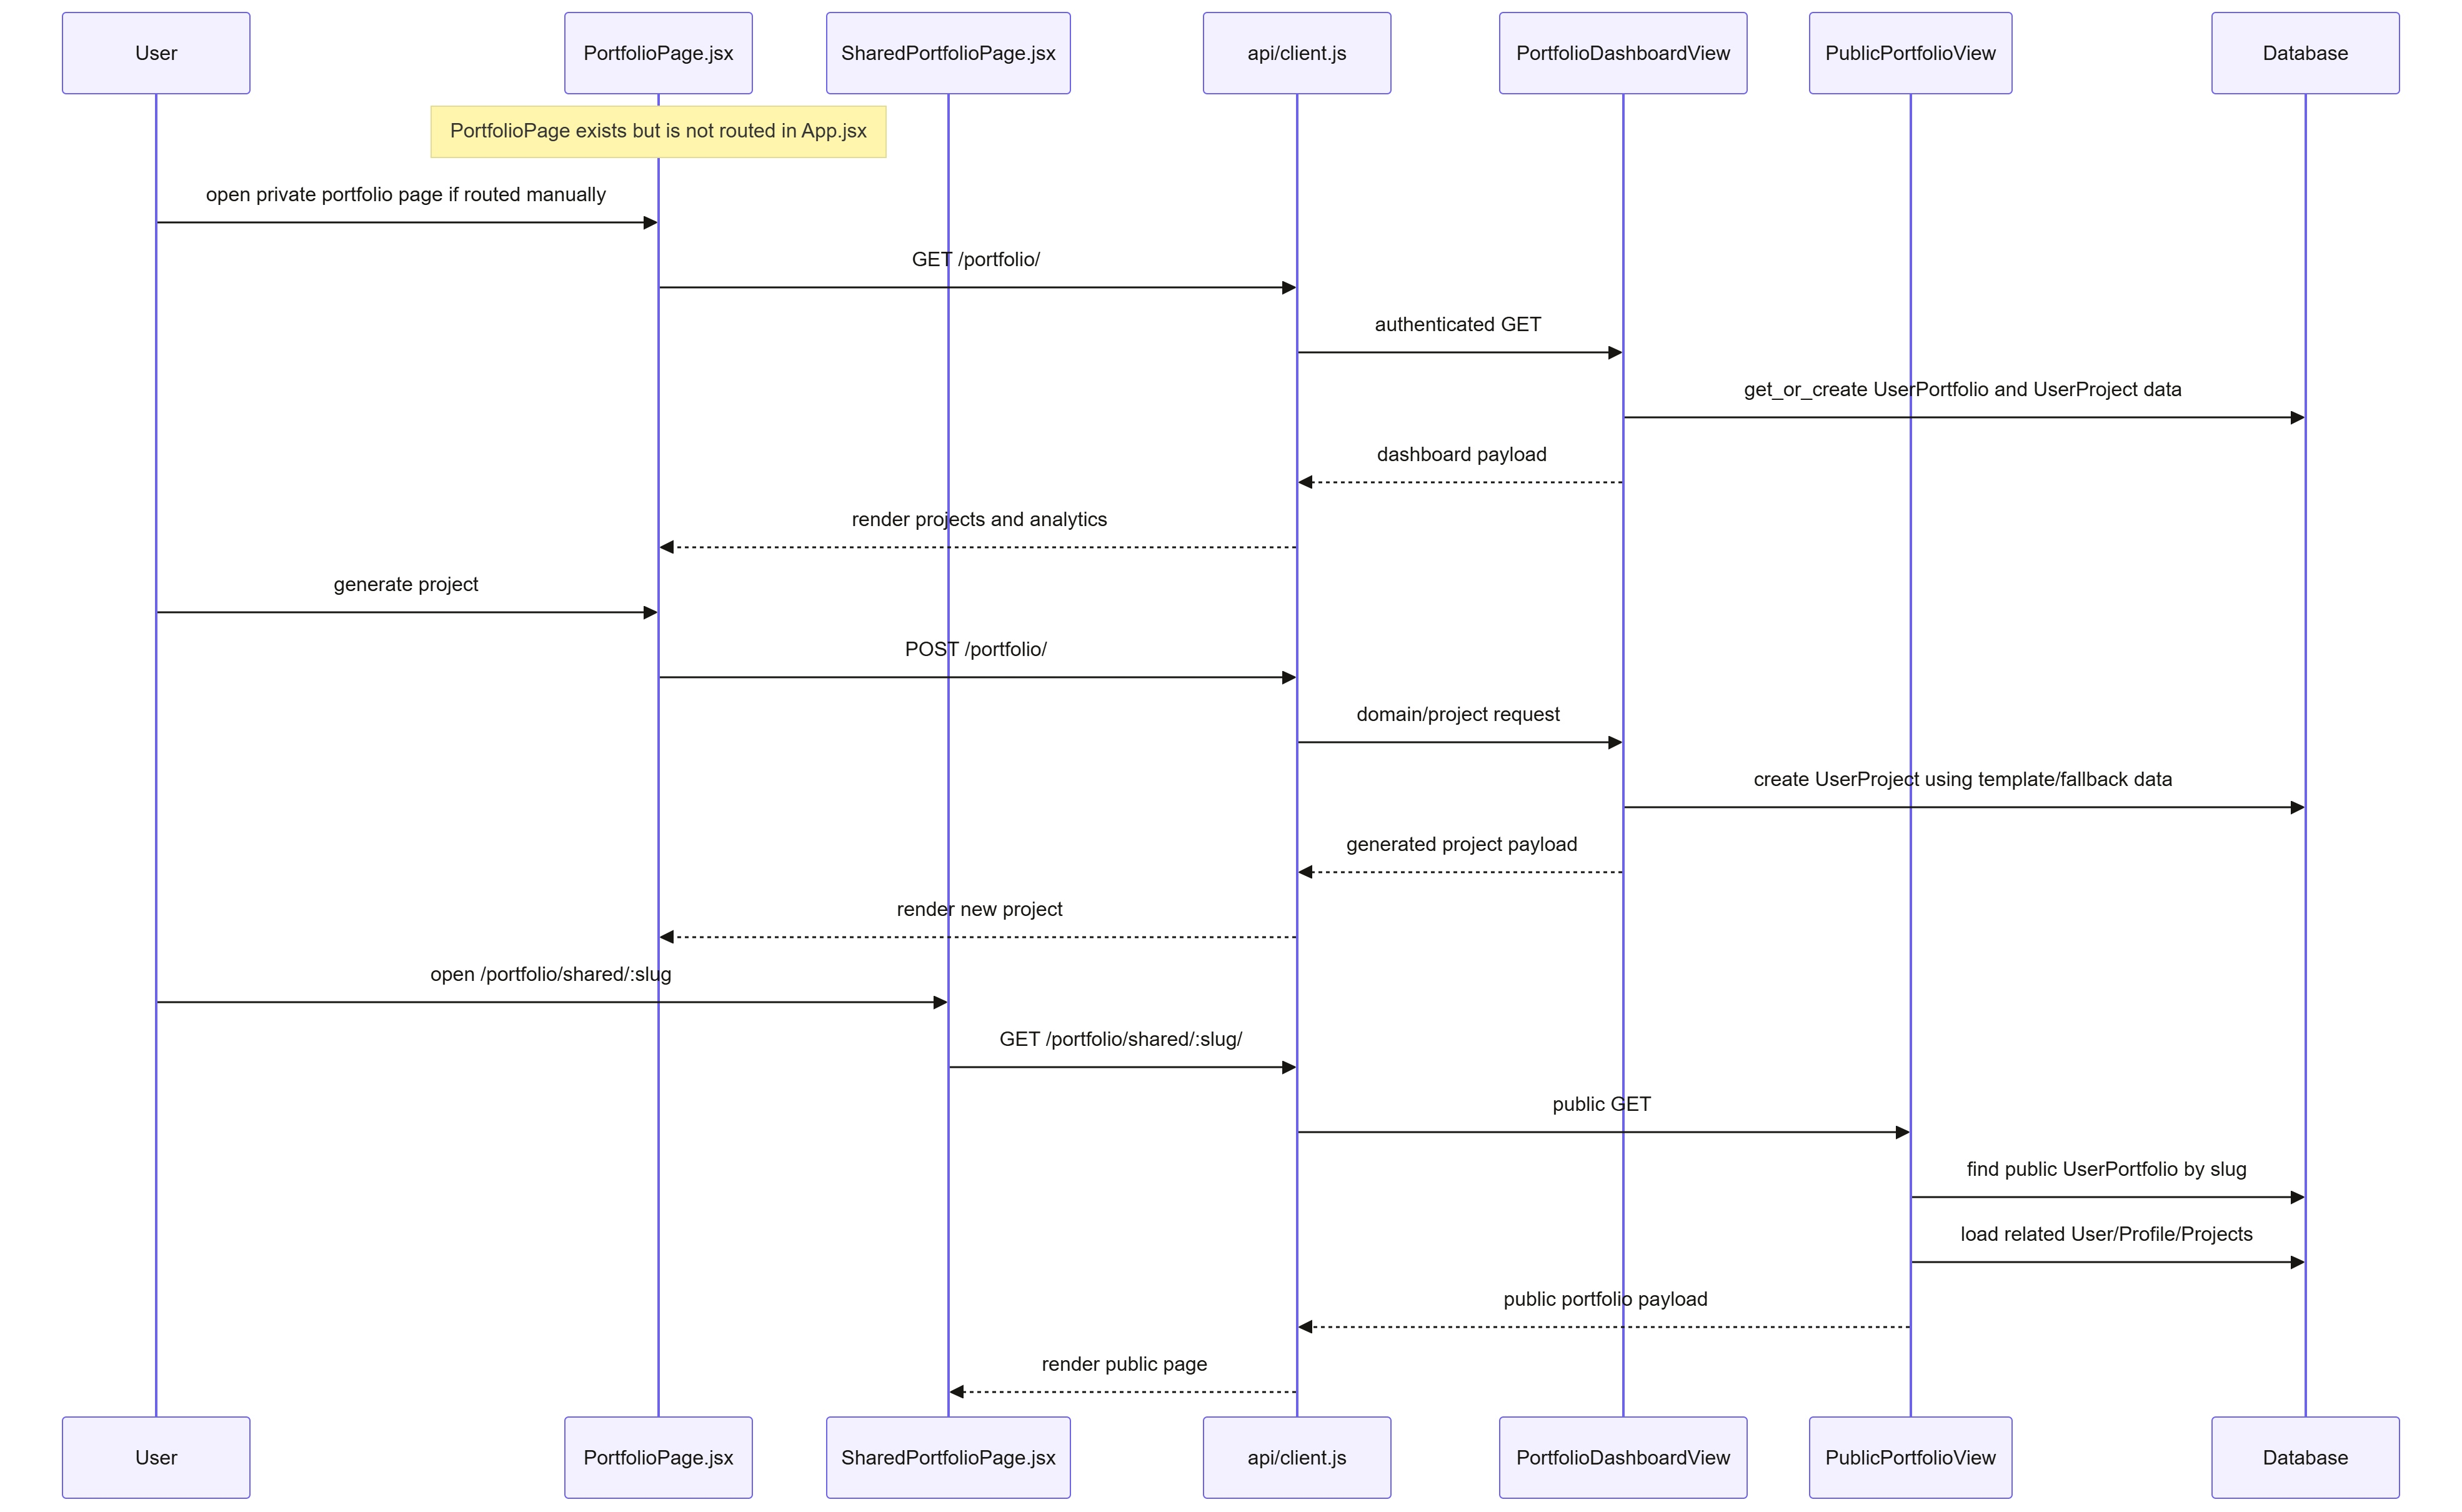
\includegraphics[width=\textwidth]{Media/Chapter 4/17 Portfolio Workflow.jpg}
\caption{Portfolio and Skills Passport Workflow}
\label{fig:portfolio_workflow}
\end{figure}

The Portfolio and Skills Passport Module begins when an authenticated student accesses the portfolio section through the frontend interface. The React application sends a request to the backend to retrieve the user's academic information, projects, certifications, technical skills, coding statistics, interview performance, and placement preparation progress.

The backend collects the required information from multiple database entities, including UserProfile, UserProject, UserCertificate, UserPassport, UserPortfolio, and other related records. These data are processed to generate a comprehensive professional profile representing the student's overall employability.

Students can further customize their portfolio by adding project descriptions, technology stacks, GitHub links, and personal achievements. The backend stores these modifications and generates a unique public URL that can be shared with recruiters or placement coordinators.

The Skills Passport is generated automatically using analytical information collected throughout the placement preparation journey. Metrics such as coding performance, interview readiness, learning progress, and technical competency are consolidated into a unified employability profile that reflects the student's current preparation status.

Whenever a recruiter or external user accesses a shared portfolio or passport link, the backend retrieves only publicly available information and renders the corresponding profile without exposing confidential user data.

\subsection{Portfolio Generation Workflow}

The Portfolio and Skills Passport Module follows the workflow below.

\begin{enumerate}

\item The student accesses the portfolio dashboard.

\item The frontend requests portfolio information.

\item The backend retrieves academic and placement data.

\item Portfolio information is generated dynamically.

\item Skills Passport metrics are calculated.

\item Public sharing links are generated.

\item Portfolio information is stored in the database.

\item Shared portfolios are displayed to authorized external users.

\end{enumerate}

\subsection{Major Features}

The Portfolio and Skills Passport Module provides the following features.

\begin{itemize}

\item Automatic portfolio generation.

\item Skills Passport generation.

\item Public portfolio sharing.

\item Project management.

\item Certification management.

\item Recruiter-friendly profile presentation.

\item Dynamic employability score generation.

\item Integration with placement analytics.

\end{itemize}

\subsection{Advantages of the Portfolio and Skills Passport Module}

The implemented module offers several advantages.

\begin{itemize}

\item Eliminates manual portfolio preparation.

\item Automatically reflects placement preparation progress.

\item Improves recruiter visibility.

\item Provides a centralized professional profile.

\item Supports public sharing through secure URLs.

\item Encourages continuous profile improvement.

\end{itemize}

\section{Company Readiness Module}

The Company Readiness Module assists students in preparing for specific companies by providing personalized preparation tracking, readiness evaluation, and company-oriented learning recommendations. Instead of following a generic preparation strategy, students can select their target companies and monitor their progress based on the requirements of each organization.

The module combines learning progress, coding performance, interview preparation, and assessment results to generate company-specific readiness information, enabling students to identify areas that require additional attention before participating in placement drives.

Figure~\ref{fig:company_readiness_workflow} illustrates the workflow of the Company Readiness Module.

\begin{figure}[H]
\centering
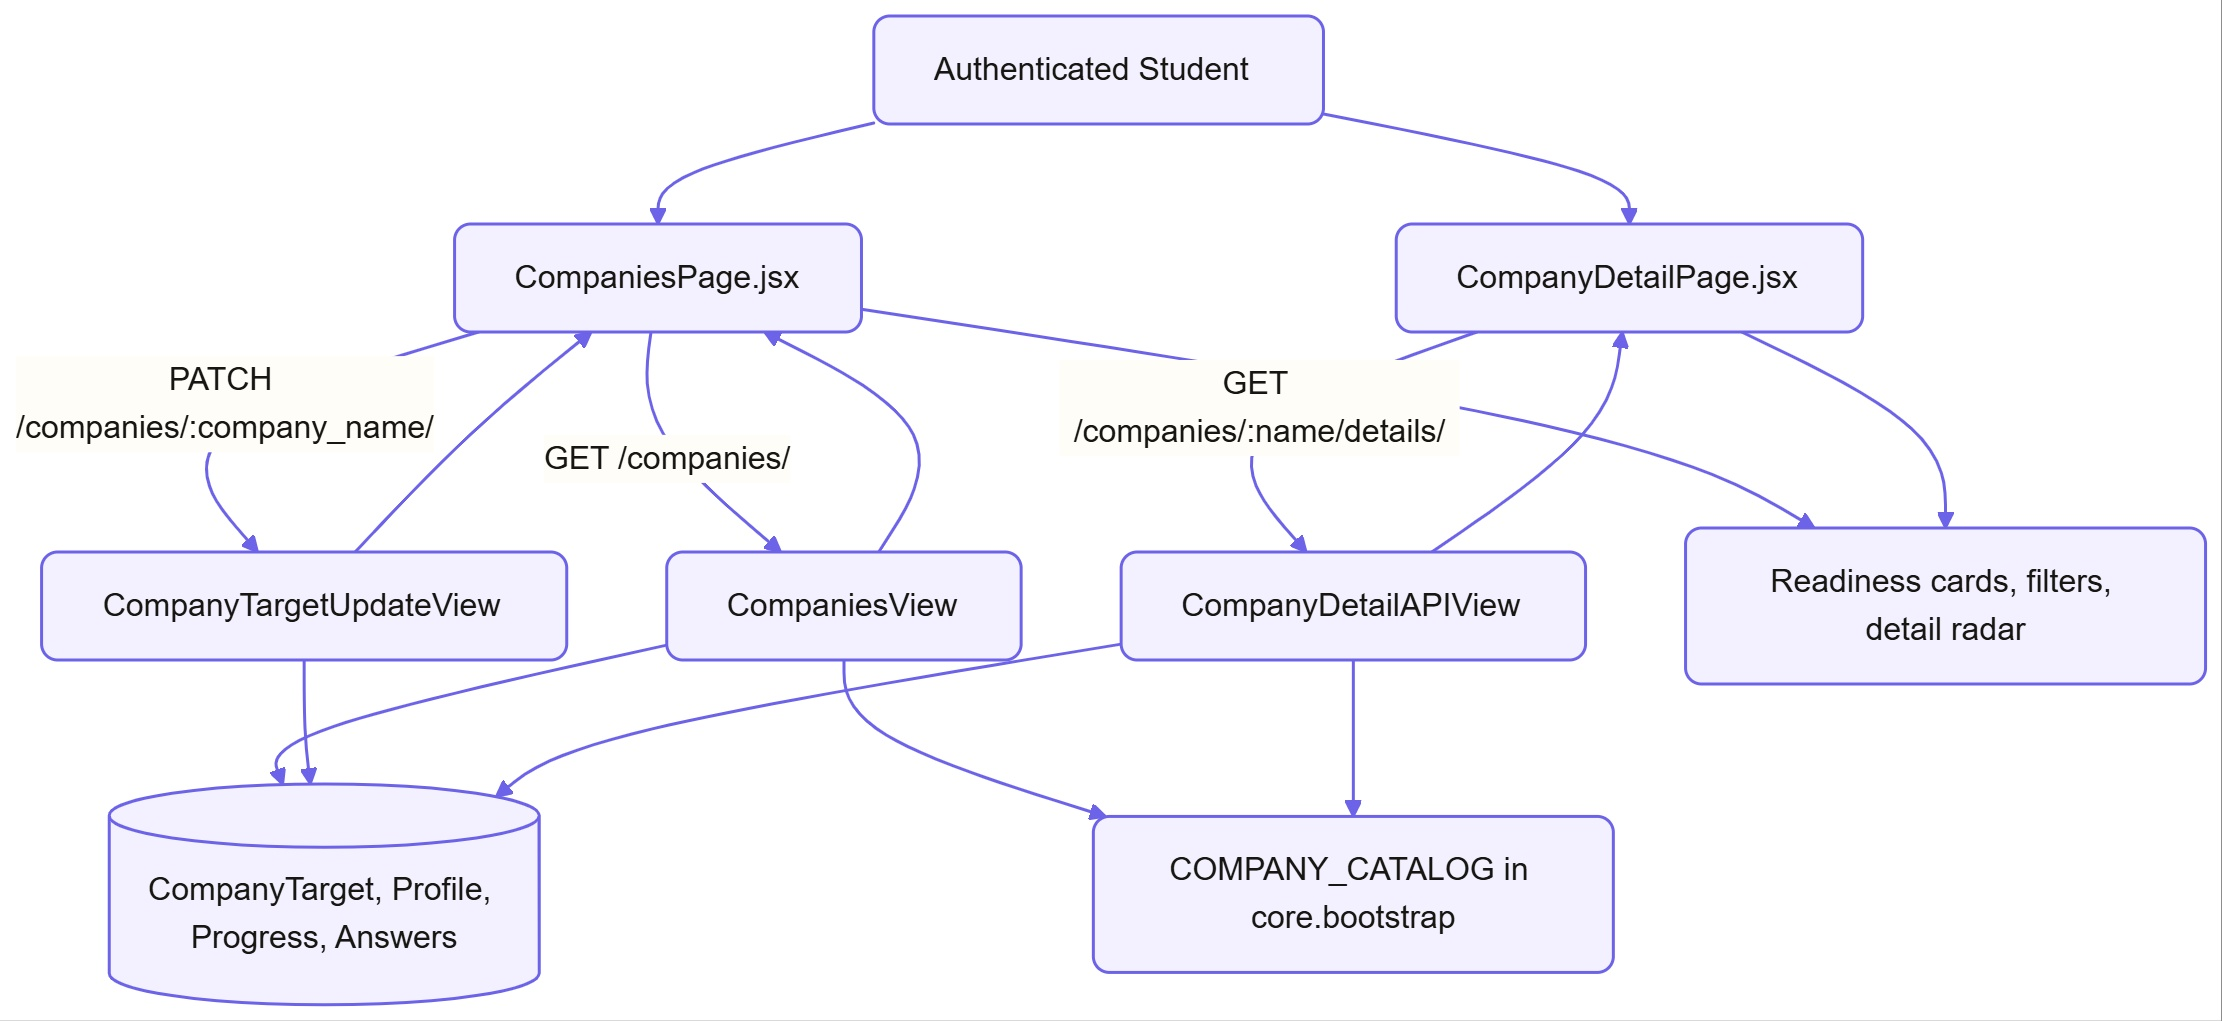
\includegraphics[width=\textwidth]{Media/Chapter 4/18 Company Readiness Workflow.jpg}
\caption{Company Readiness Workflow}
\label{fig:company_readiness_workflow}
\end{figure}

The Company Readiness Module begins when an authenticated student selects a target company through the frontend interface. The React application requests company-specific information from the backend, including preparation requirements, recommended topics, coding difficulty, interview expectations, and readiness metrics.

The backend retrieves the selected company's preparation profile together with the student's learning progress, coding submissions, quiz performance, interview results, and completed learning topics. These records are analyzed to calculate the student's readiness level for the selected company.

Based on the calculated readiness score, the module identifies completed requirements, pending topics, weak subject areas, and recommended activities. The generated information is returned to the frontend, where it is presented using progress indicators, readiness cards, and detailed preparation summaries.

Whenever the student completes additional learning activities, coding problems, or mock interviews, the readiness score is automatically recalculated, ensuring that the displayed information always reflects the student's current preparation status.

\subsection{Company Readiness Workflow}

The Company Readiness Module follows the sequence below.

\begin{enumerate}

\item The student selects a target company.

\item The frontend requests company preparation details.

\item The backend retrieves the student's preparation records.

\item Company requirements are compared with the student's progress.

\item Readiness scores are calculated.

\item Weak areas and pending topics are identified.

\item Personalized recommendations are generated.

\item The frontend displays the updated company readiness dashboard.

\end{enumerate}

\subsection{Major Features}

The Company Readiness Module provides the following features.

\begin{itemize}

\item Company-specific preparation tracking.

\item Personalized readiness score calculation.

\item Topic recommendation based on company requirements.

\item Coding readiness analysis.

\item Interview readiness evaluation.

\item Progress visualization.

\item Automatic readiness updates.

\item Integration with dashboard analytics.

\end{itemize}

\subsection{Advantages of the Company Readiness Module}

The implemented module provides several advantages.

\begin{itemize}

\item Supports focused preparation for individual companies.

\item Helps students identify preparation gaps.

\item Provides personalized learning recommendations.

\item Continuously updates readiness scores.

\item Integrates multiple preparation activities into a unified evaluation.

\item Improves placement preparation efficiency.

\end{itemize}

\section{Chapter Summary}

This chapter described the implementation of the PrepSmart platform, including the technologies, development environment, frontend architecture, backend architecture, authentication mechanism, placement preparation workflow, dashboard analytics, mock test module, AI interview module, coding practice environment, portfolio and skills passport generation, and company readiness module.

The implementation follows a modular client--server architecture developed using React, Django, Django REST Framework, and MySQL. The integration of AI-assisted interview evaluation, coding practice, personalized analytics, and company-specific preparation provides students with a comprehensive placement preparation ecosystem.

The next chapter presents the results of the developed system through screenshots of the implemented user interfaces and demonstrates the practical functionality of each module.
    \chapter{Results and User Interface}

\section{Introduction}

This chapter presents the implementation results of the proposed Smart Placement Preparation Platform (PrepSmart) through the developed user interfaces. The screenshots included in this chapter demonstrate the major functionalities implemented during the development of the system and illustrate how users interact with different modules of the application.

The platform provides a modern and intuitive web interface that enables students to access placement preparation resources through a single integrated application. The implemented modules include user authentication, personalized dashboards, structured learning paths, coding practice, mock assessments, AI-assisted interview preparation, company-specific readiness analysis, portfolio management, skills passport generation, analytics, and administrative tools.

Each section of this chapter presents the corresponding user interface along with a detailed explanation of its functionality, highlighting how the developed system addresses the challenges identified during the requirement analysis phase.

\section{Landing Page}

The landing page serves as the public entry point of the PrepSmart platform. It introduces visitors to the objectives, major features, and capabilities of the application before authentication. The page is designed to provide a professional first impression while allowing users to easily navigate to the registration or login pages.

The interface follows a clean and responsive design, ensuring compatibility across different screen sizes and devices. Important features of the platform are highlighted using descriptive sections and interactive components, enabling prospective users to understand the purpose of the system before creating an account.

\begin{figure}[H]
\centering
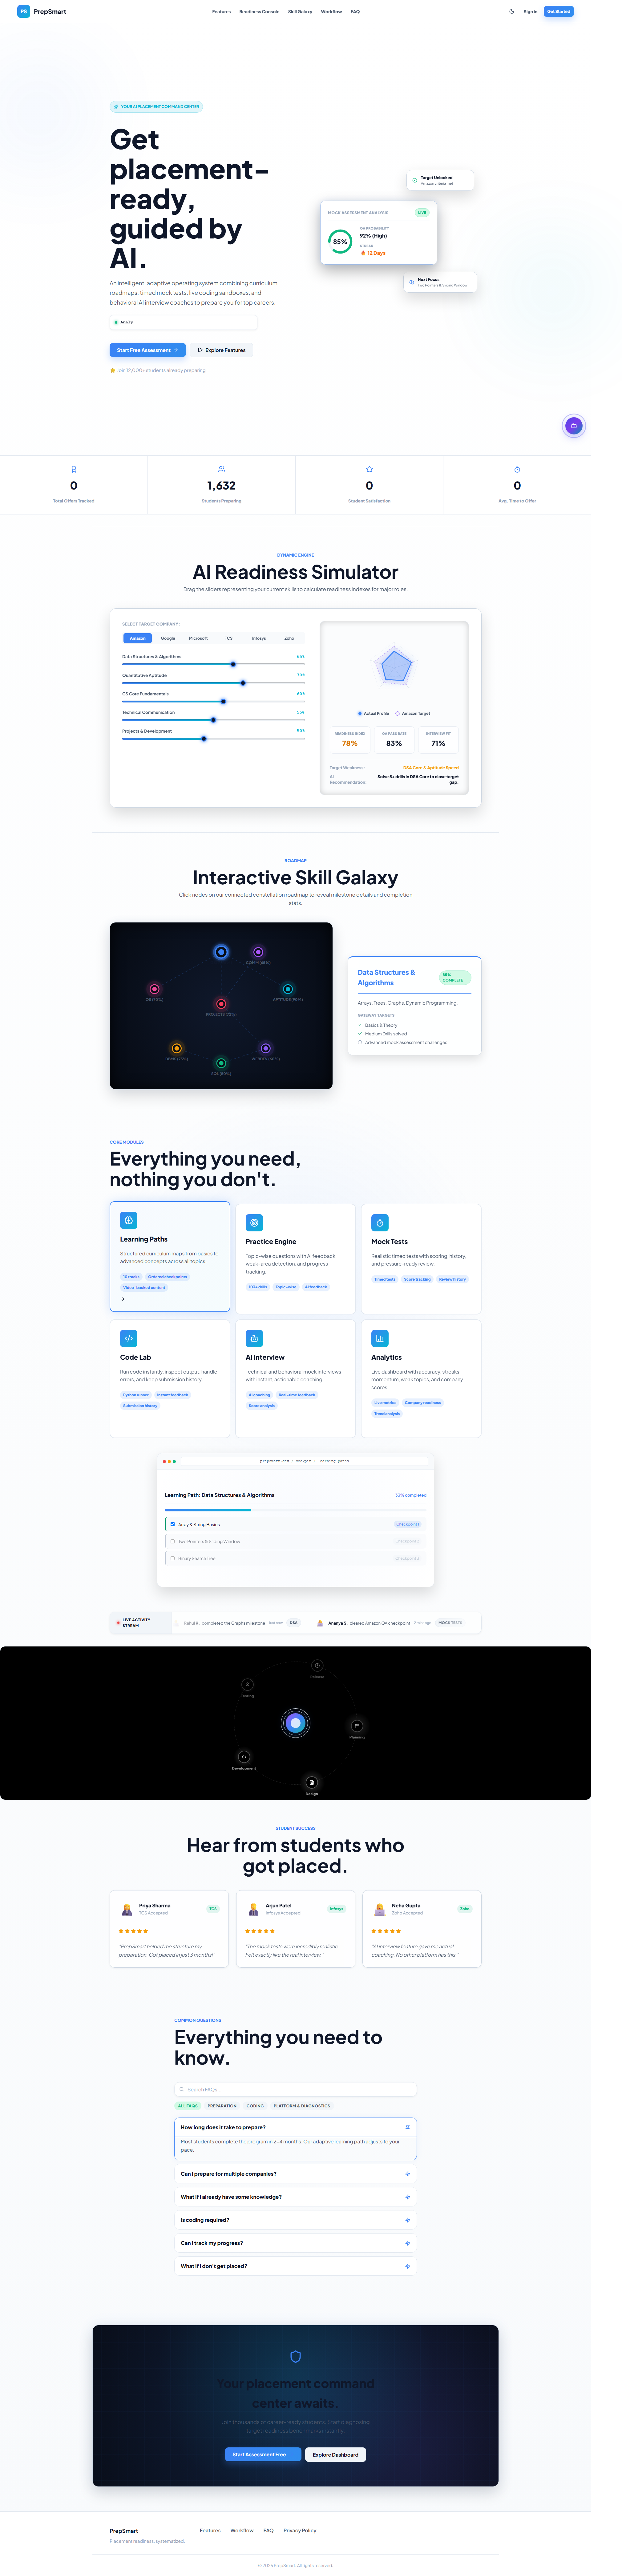
\includegraphics[width=0.70\textwidth]{Media/Chapter 5/landing.png}
\caption{Landing Page of PrepSmart}
\label{fig:landing_page}
\end{figure}

Figure~\ref{fig:landing_page} illustrates the landing page presented to users when they access the PrepSmart platform. The homepage introduces the application and highlights its primary objective of providing a unified environment for placement preparation.

The navigation menu provides quick access to important sections of the application, while prominent action buttons allow users to register for a new account or log into an existing account. The landing page also presents the core features offered by the platform, including structured learning paths, coding practice, mock tests, AI-powered interview preparation, company readiness tracking, portfolio generation, and performance analytics.

The responsive layout ensures consistent presentation across desktop and mobile devices. Visual elements, icons, and feature cards improve usability and make the interface easy to understand for first-time users. Overall, the landing page serves as the gateway to the platform and effectively communicates the functionality and benefits of PrepSmart.

\subsection{Major Features of the Landing Page}

The landing page provides the following features:

\begin{itemize}

\item Introduction to the PrepSmart platform.

\item Navigation to login and registration pages.

\item Overview of the major placement preparation modules.

\item Responsive and user-friendly interface.

\item Professional presentation of platform capabilities.

\item Quick access to important information for new users.

\end{itemize}

\subsection{Advantages}

The landing page offers several advantages:

\begin{itemize}

\item Creates a professional first impression.

\item Clearly communicates the purpose of the platform.

\item Simplifies navigation for new users.

\item Highlights the major features available after authentication.

\item Provides a responsive interface for different devices.

\end{itemize}

\section{User Authentication}

User authentication is the first step in accessing the personalized features of the PrepSmart platform. The authentication module ensures that only registered users can access protected resources such as dashboards, learning modules, coding practice, AI interviews, company readiness tracking, and profile management.

The platform provides separate interfaces for user login and new user registration. Both interfaces are designed to be simple, responsive, and user-friendly while ensuring secure authentication using JSON Web Tokens (JWT).

\subsection{Login Page}

The login page allows registered users to securely access the PrepSmart platform by verifying their credentials. The interface is designed to provide a simple and intuitive authentication experience while maintaining application security.

\begin{figure}[H]
\centering
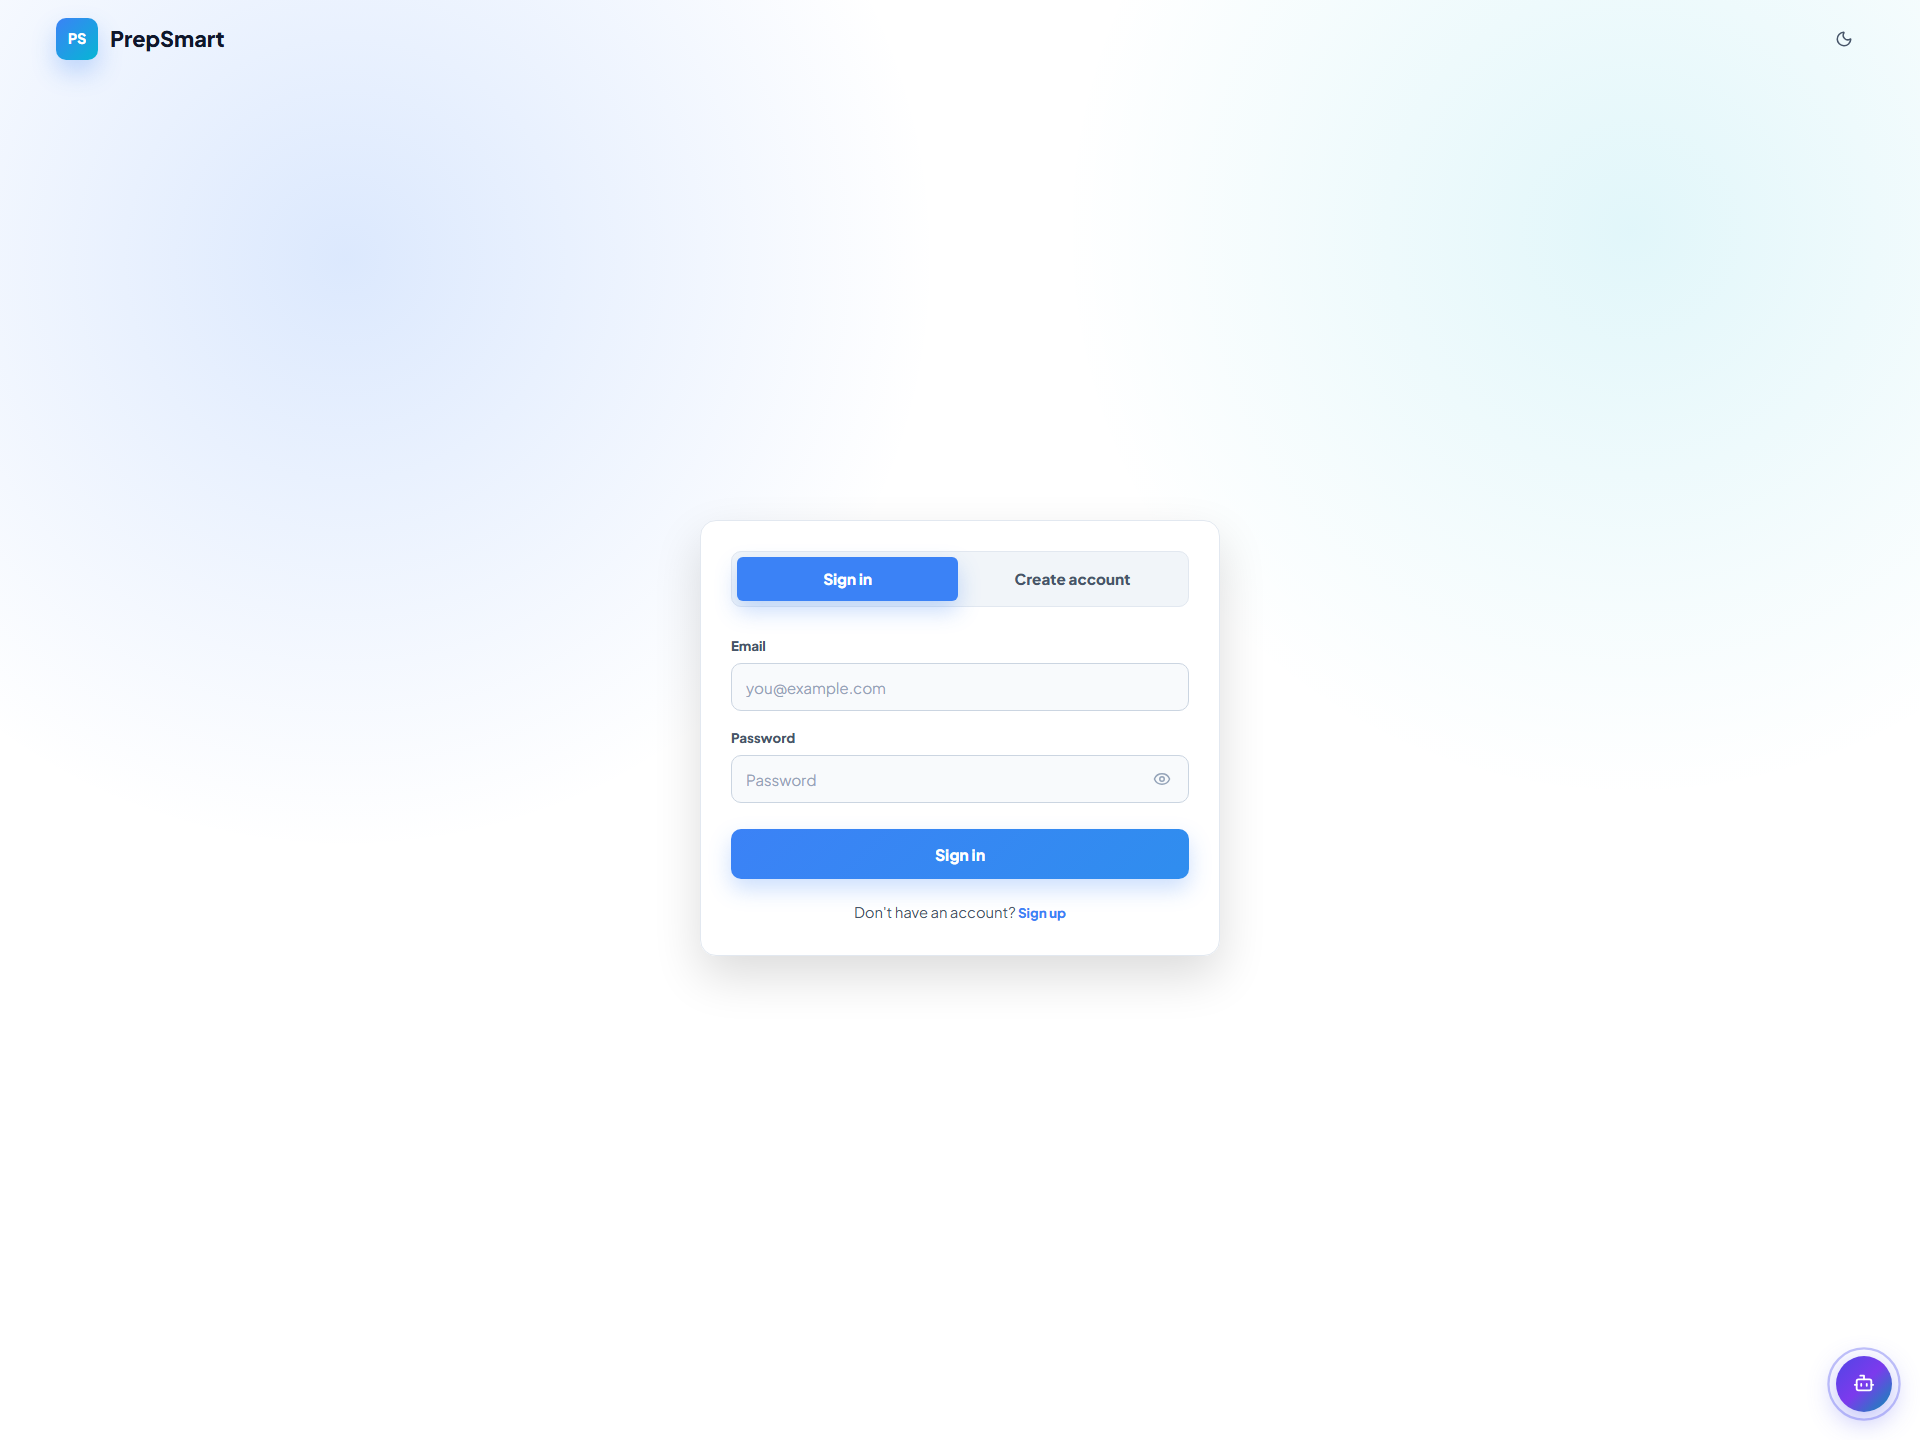
\includegraphics[width=\textwidth]{Media/Chapter 5/login.png}
\caption{Login Page}
\label{fig:login_page}
\end{figure}

Figure~\ref{fig:login_page} shows the login interface of PrepSmart. Registered users enter their email address and password to authenticate themselves before accessing the platform. After successful authentication, the system generates a JSON Web Token (JWT) and redirects the user to the personalized dashboard.

The login interface includes input fields for user credentials along with validation mechanisms that prevent invalid or incomplete submissions. Appropriate error messages are displayed whenever incorrect credentials are entered, enabling users to correct their information before attempting to log in again.

The interface follows a clean and responsive design that ensures consistent usability across different devices. Once authenticated, users gain access to all modules associated with their account, including placement preparation, coding practice, AI interview sessions, portfolio management, and analytics.

\subsubsection*{Major Features}

\begin{itemize}

\item Secure user authentication.

\item Email and password validation.

\item JWT-based session management.

\item Error handling for invalid credentials.

\item Responsive and user-friendly interface.

\item Direct navigation to the dashboard after successful login.

\end{itemize}

\subsection{Registration Page}

The registration page enables new users to create an account on the PrepSmart platform. The interface collects the required personal and academic information before securely creating a new user profile.

\begin{figure}[H]
\centering
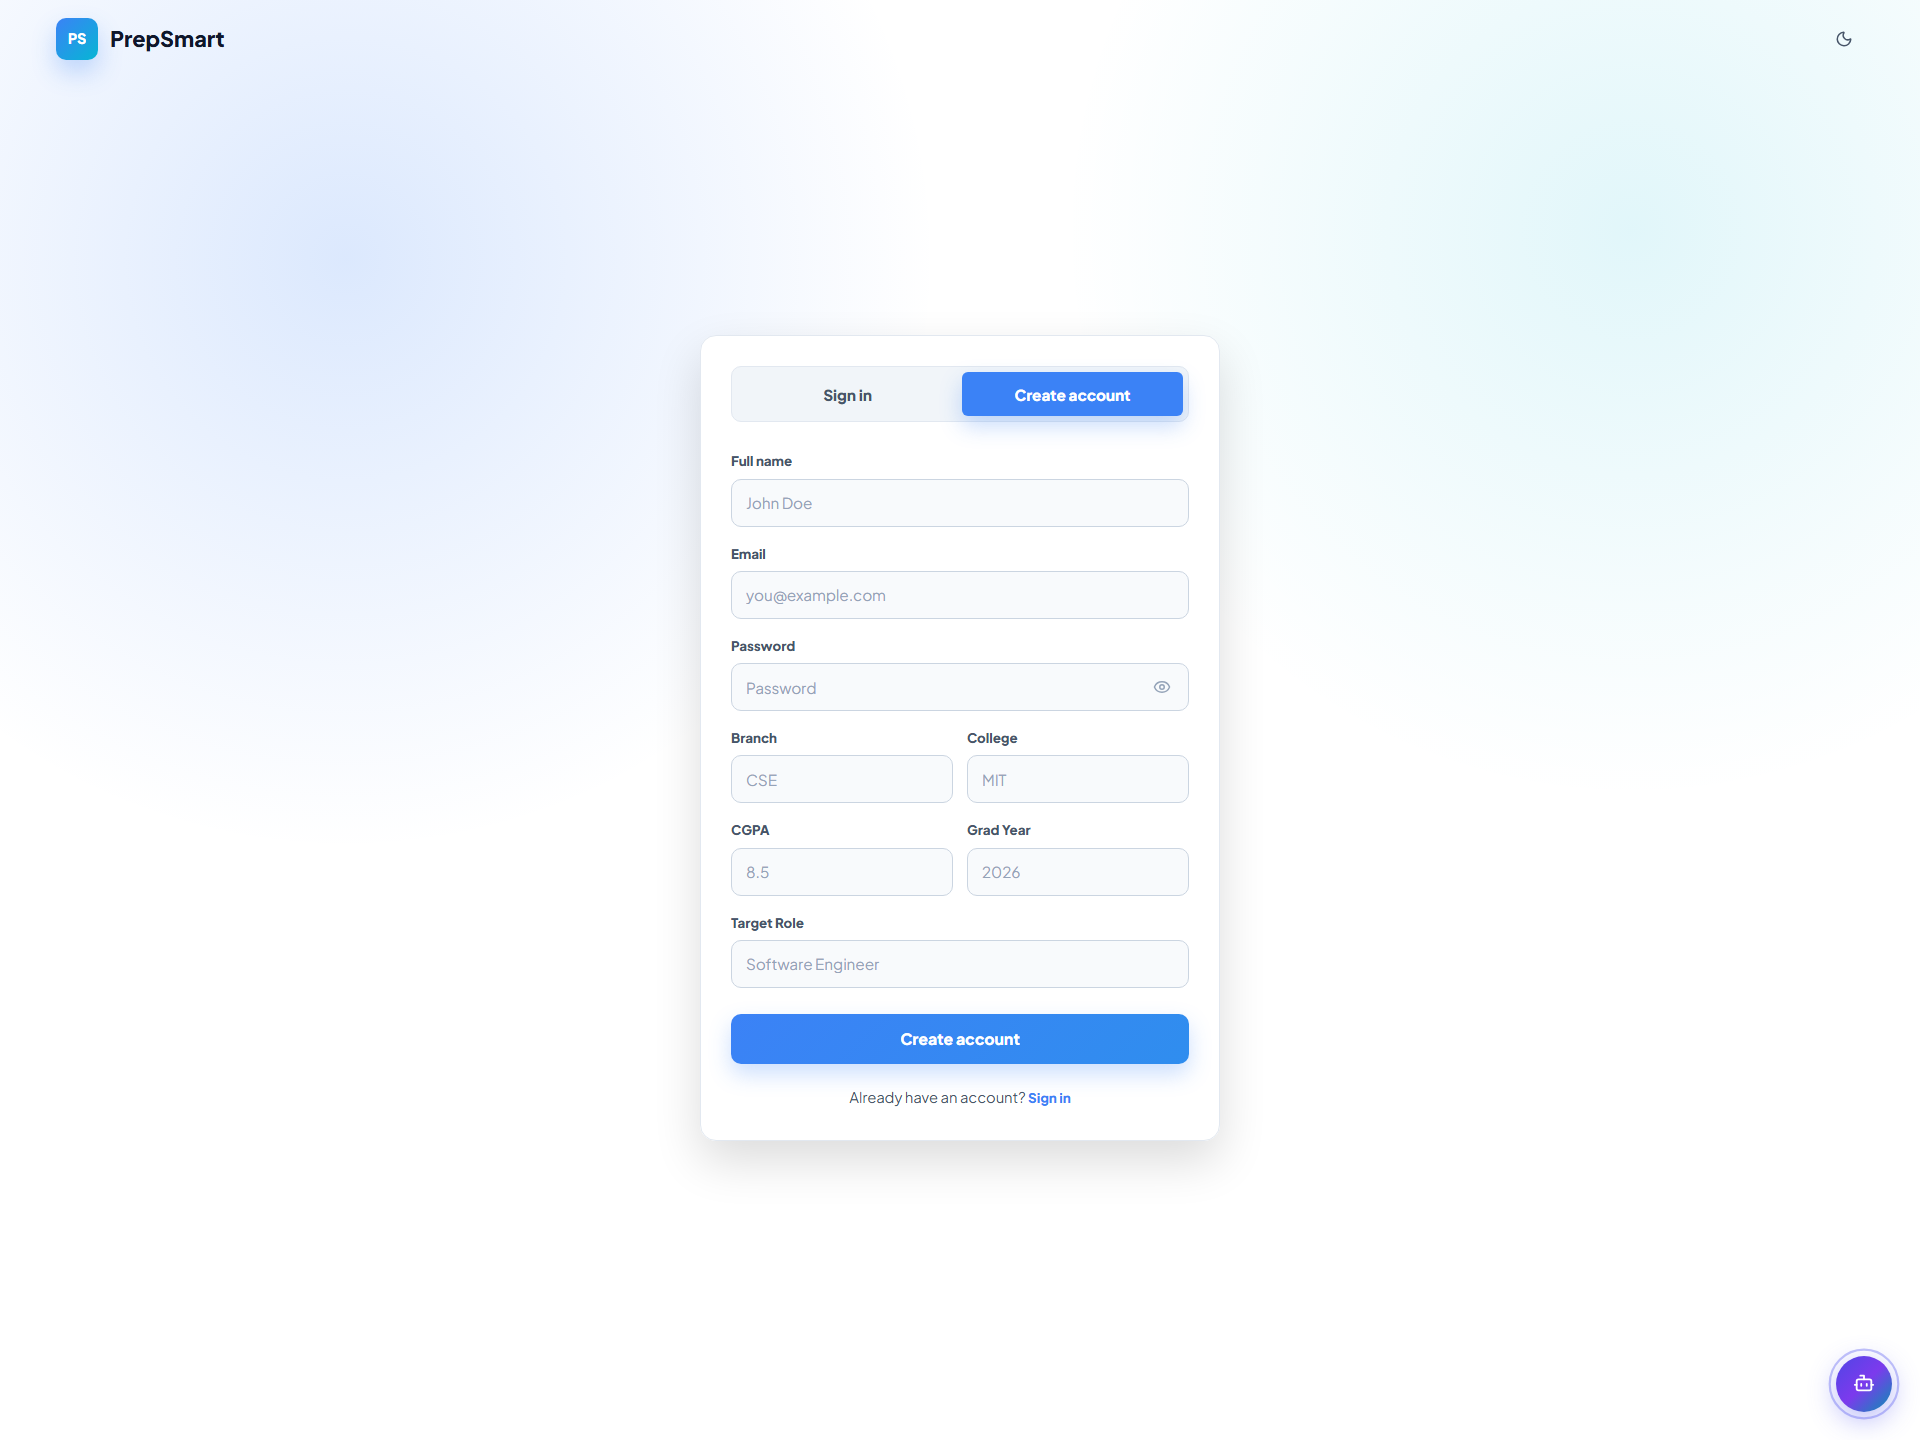
\includegraphics[width=\textwidth]{Media/Chapter 5/signup.png}
\caption{User Registration Page}
\label{fig:signup_page}
\end{figure}

Figure~\ref{fig:signup_page} illustrates the user registration interface of PrepSmart. New users provide the required information such as name, email address, password, and other registration details to create an account.

Before creating the account, the backend validates the submitted information to ensure that mandatory fields are completed correctly and that duplicate accounts are not created. Upon successful registration, a new user profile is generated and stored in the database.

The registration interface is designed to minimize complexity while providing sufficient validation to maintain data integrity. Once registration is completed successfully, users can log into the platform using their newly created credentials and begin their placement preparation journey.

\subsubsection*{Major Features}

\begin{itemize}

\item New user registration.

\item Input validation.

\item Duplicate account prevention.

\item Secure password handling.

\item Automatic user profile creation.

\item Integration with JWT authentication.

\end{itemize}

\section{Dashboard}

The Dashboard serves as the central workspace of the PrepSmart platform. After successful authentication, users are redirected to this page, where they can monitor their overall placement preparation progress through a unified and interactive interface. The dashboard consolidates information from multiple modules, including learning progress, coding practice, mock tests, interview preparation, company readiness, and daily goals.

The dashboard is designed to provide students with an overview of their current preparation status, helping them identify completed activities, pending tasks, and areas requiring improvement. Instead of navigating through multiple pages, users can quickly access the most important information from a single interface.

\begin{figure}[H]
\centering
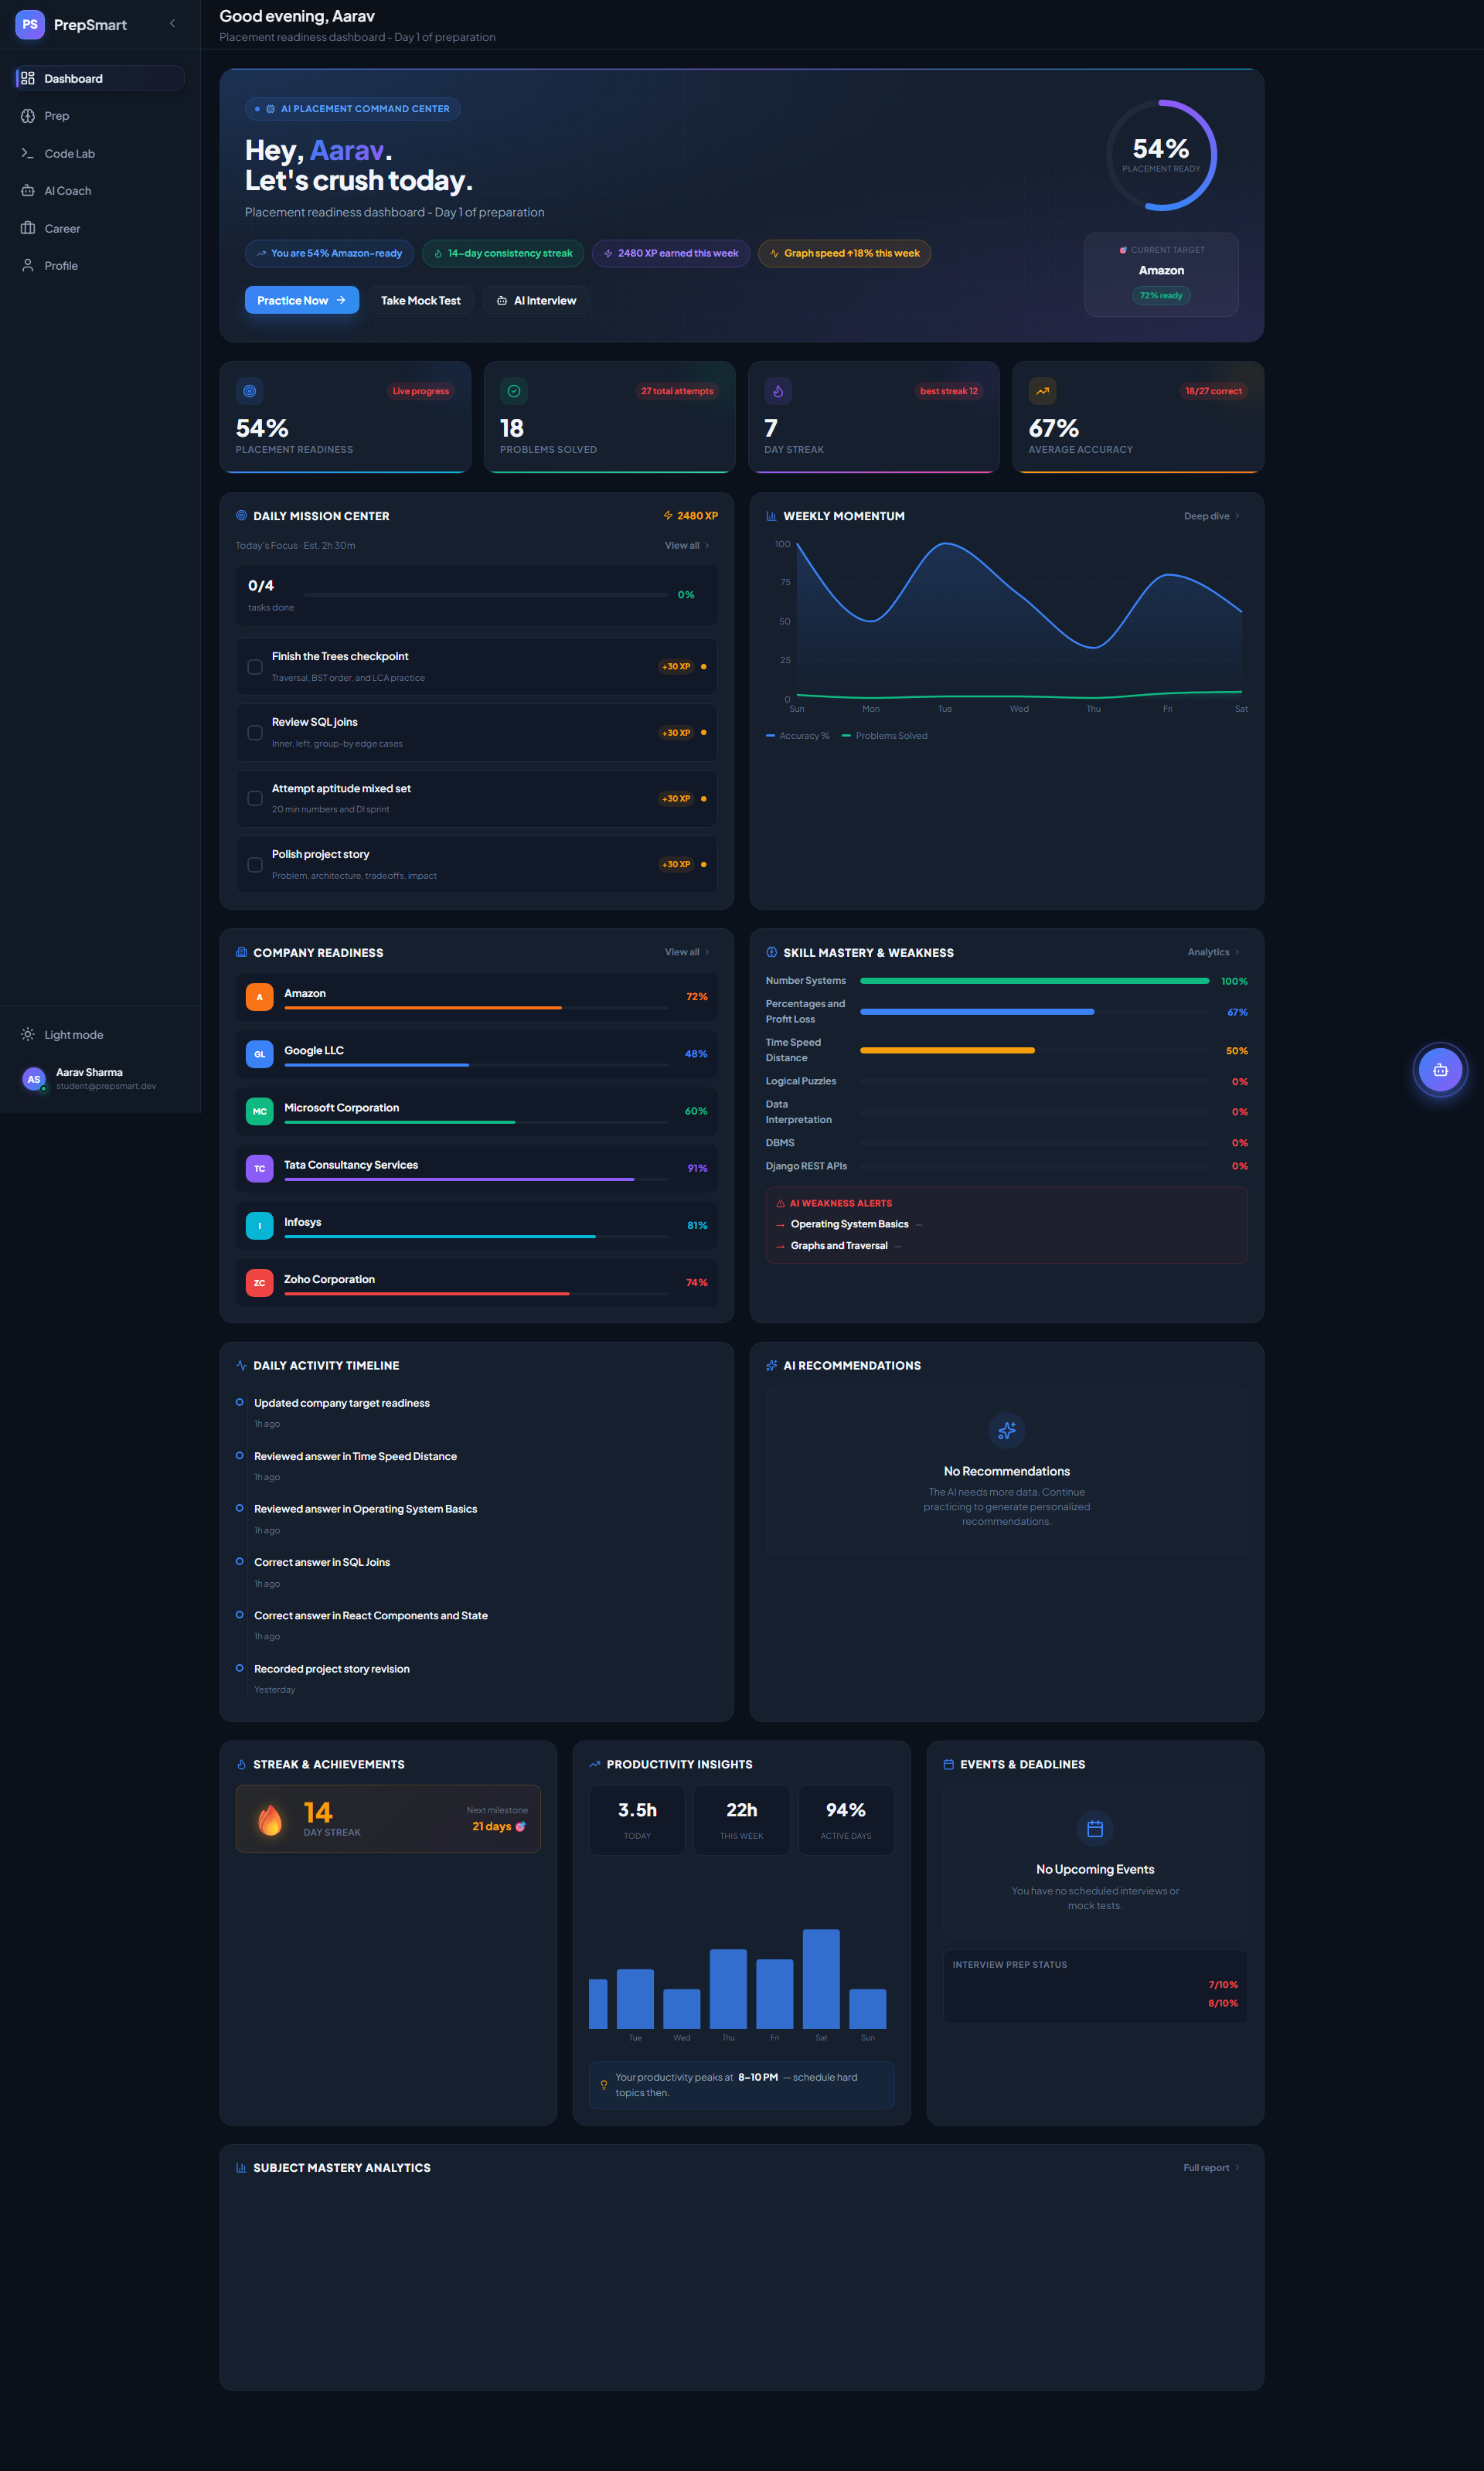
\includegraphics[width=0.95\textwidth]{Media/Chapter 5/dashboard.png}
\caption{Student Dashboard}
\label{fig:dashboard}
\end{figure}

Figure~\ref{fig:dashboard} illustrates the main dashboard of the PrepSmart platform. After authentication, this page acts as the personalized homepage for every student. The dashboard aggregates information from different modules and presents it in an organized manner using cards, charts, progress indicators, and statistical summaries.

The upper section of the dashboard displays important performance metrics such as placement readiness, completed topics, coding activity, interview progress, and overall learning statistics. These indicators are updated automatically whenever the student completes learning activities, coding problems, mock tests, or interview sessions.

The central portion of the dashboard provides quick access to active learning tracks, daily goals, recent activities, recommended topics, and upcoming preparation milestones. This allows students to continue their preparation without manually searching for unfinished tasks.

The dashboard also includes visual analytics that summarize preparation progress using graphs and progress bars. These visualizations help students understand their strengths and weaknesses while enabling continuous monitoring of their placement readiness. Since all information is retrieved dynamically from the backend database, the dashboard always reflects the latest progress of the student.

\subsection{Major Components of the Dashboard}

The dashboard consists of several important components that assist students during placement preparation.

\begin{itemize}

\item Personalized welcome section.

\item Overall placement readiness score.

\item Learning progress indicators.

\item Coding practice statistics.

\item Mock test performance summary.

\item AI interview readiness information.

\item Daily learning goals.

\item Activity history.

\item Recommended learning tasks.

\item Navigation shortcuts to major modules.

\end{itemize}

\subsection{Functionalities}

The Dashboard provides the following functionalities:

\begin{itemize}

\item Displays real-time preparation statistics.

\item Tracks completion of learning topics.

\item Shows coding practice performance.

\item Monitors interview readiness.

\item Displays company preparation status.

\item Provides personalized recommendations.

\item Enables quick navigation to learning modules.

\item Updates automatically after every completed activity.

\end{itemize}

\subsection{Advantages}

The Dashboard offers several advantages to students preparing for campus placements.

\begin{itemize}

\item Centralized view of placement preparation.

\item Real-time progress monitoring.

\item Easy identification of weak areas.

\item Better learning organization.

\item Improved motivation through progress visualization.

\item Efficient access to all major platform modules.

\end{itemize}

\section{Placement Preparation Module}

The Placement Preparation Module is the primary learning component of PrepSmart. It provides students with a structured and organized approach towards campus placement preparation by combining learning paths, milestone tracking, topic-wise study materials, and continuous progress monitoring within a single platform.

Unlike traditional preparation methods that require students to use multiple websites, this module integrates all essential learning resources into one environment. Students can systematically complete learning tracks, monitor their progress, and prepare for technical interviews in a guided manner.

The module consists of four major interfaces: Prep Journey, Learning Roadmaps, Milestones, and Topic Study. Each interface contributes to different stages of the student's preparation process.

\subsection{Prep Journey}

The Prep Journey interface provides students with a personalized learning roadmap that organizes placement preparation into structured tracks and learning stages. It enables users to monitor completed topics, pending activities, and overall preparation progress.

\begin{figure}[H]
\centering
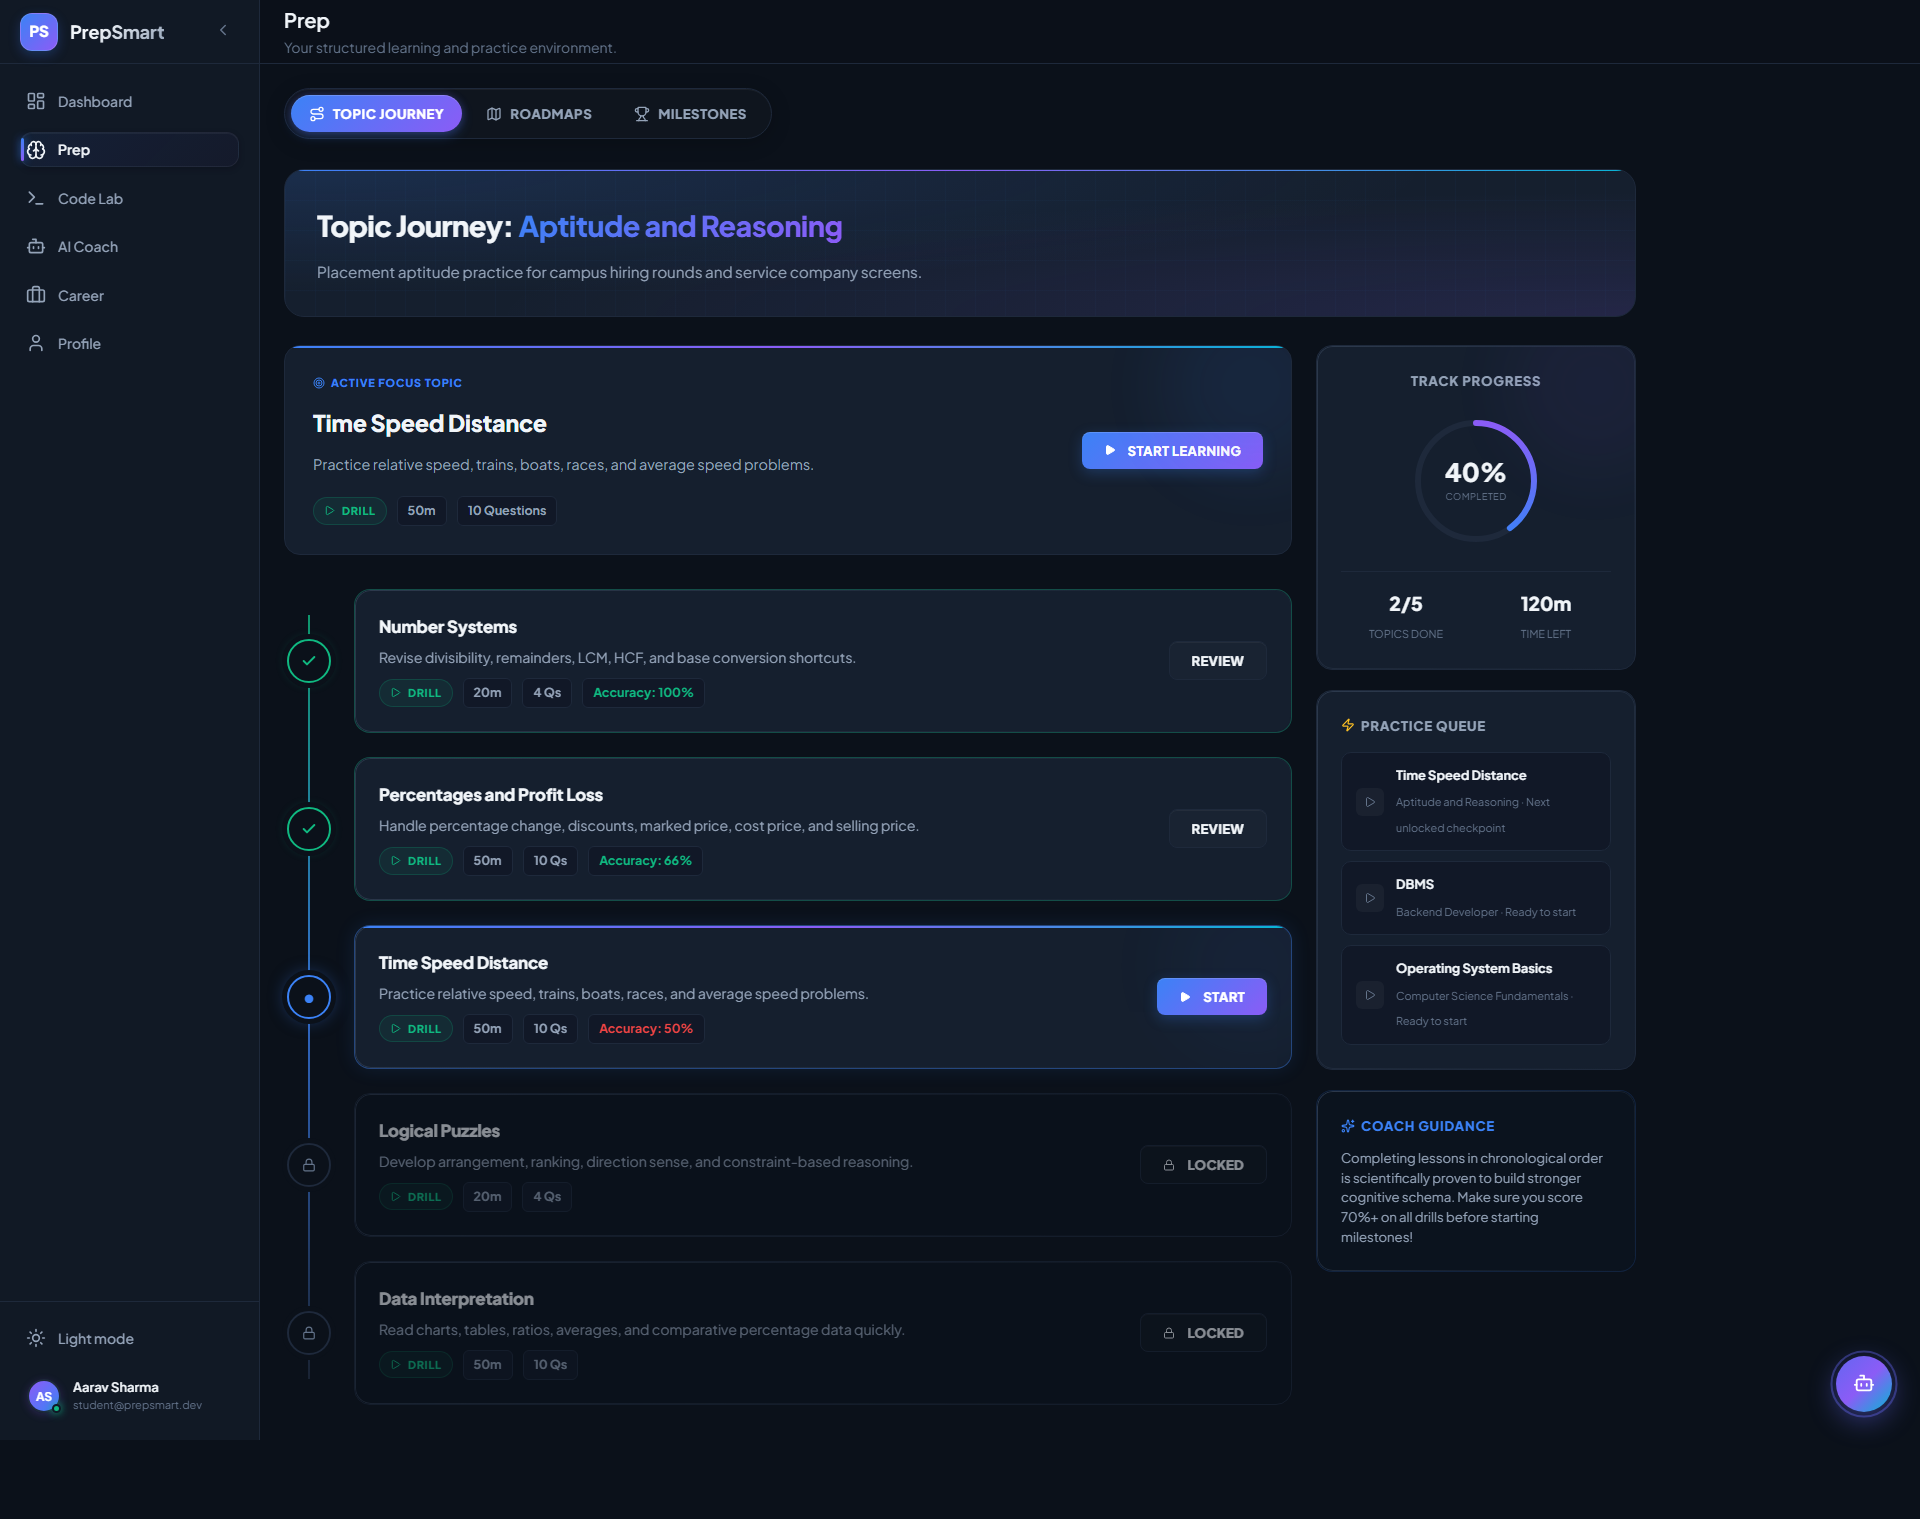
\includegraphics[width=0.95\textwidth]{Media/Chapter 5/prep_journey.png}
\caption{Prep Journey Interface}
\label{fig:prep_journey}
\end{figure}

Figure~\ref{fig:prep_journey} illustrates the Prep Journey interface of PrepSmart. This page acts as the student's personalized learning roadmap by presenting different preparation tracks in a well-organized manner.

Each learning track contains multiple topics arranged according to their recommended learning sequence. As students complete individual topics and assessments, their progress is automatically updated and reflected within the interface. This enables users to clearly distinguish between completed topics, ongoing learning activities, and pending preparation tasks.

The interface also recommends the next learning objective based on the student's previous progress, allowing users to follow a continuous and systematic preparation strategy without manually planning their studies.

\subsubsection*{Major Features}

\begin{itemize}

\item Structured learning tracks.

\item Topic completion tracking.

\item Progress visualization.

\item Personalized learning recommendations.

\item Automatic learning sequence management.

\item Integration with dashboard analytics.

\end{itemize}

\subsection{Learning Roadmaps}

The Learning Roadmaps interface presents detailed preparation paths for various placement domains. Each roadmap guides students through the recommended order of topics required to develop strong technical knowledge before attending placement interviews.

\begin{figure}[H]
\centering
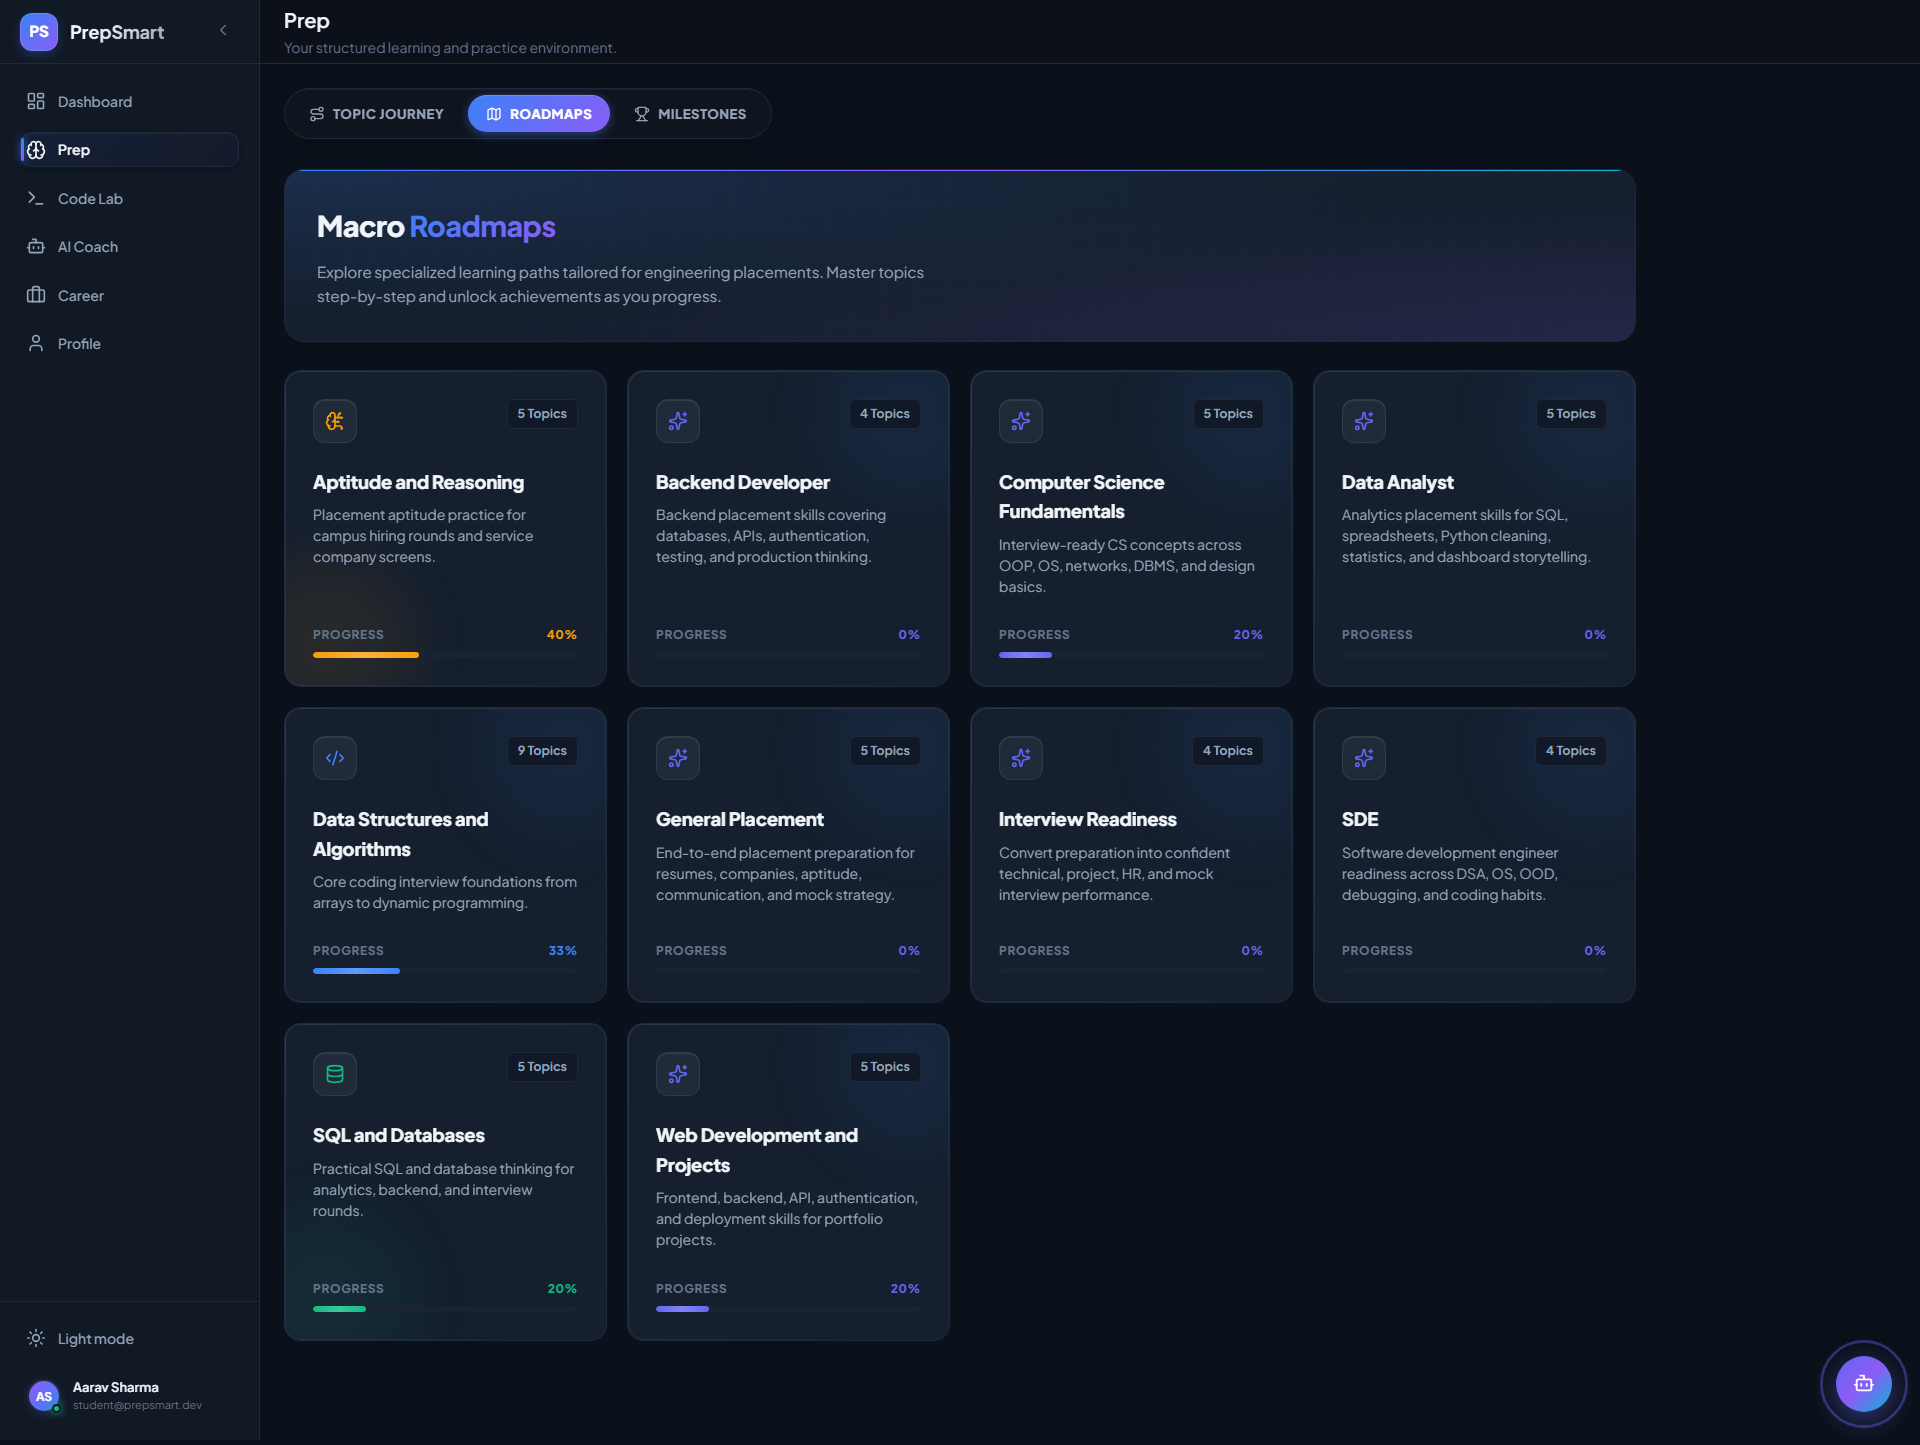
\includegraphics[width=0.95\textwidth]{Media/Chapter 5/roadmaps.png}
\caption{Learning Roadmaps}
\label{fig:learning_roadmaps}
\end{figure}

Figure~\ref{fig:learning_roadmaps} presents the Learning Roadmaps available within PrepSmart. The page organizes learning content into multiple preparation paths, allowing students to focus on specific technical domains based on their placement goals.

Each roadmap contains an ordered sequence of learning topics designed to gradually increase the student's understanding from fundamental concepts to advanced interview-level knowledge. Students can select individual roadmaps according to their interests and preparation requirements.

The roadmap interface simplifies long-term planning by clearly indicating learning dependencies and recommended study sequences.

\subsubsection*{Major Features}

\begin{itemize}

\item Domain-specific learning paths.

\item Sequential topic organization.

\item Guided placement preparation.

\item Easy roadmap navigation.

\item Progress monitoring.

\item Future learning recommendations.

\end{itemize}

\subsection{Milestones}

The Milestones interface enables students to evaluate their preparation by completing predefined learning checkpoints. These milestones divide the preparation journey into manageable stages, allowing continuous assessment of learning progress.

\begin{figure}[H]
\centering
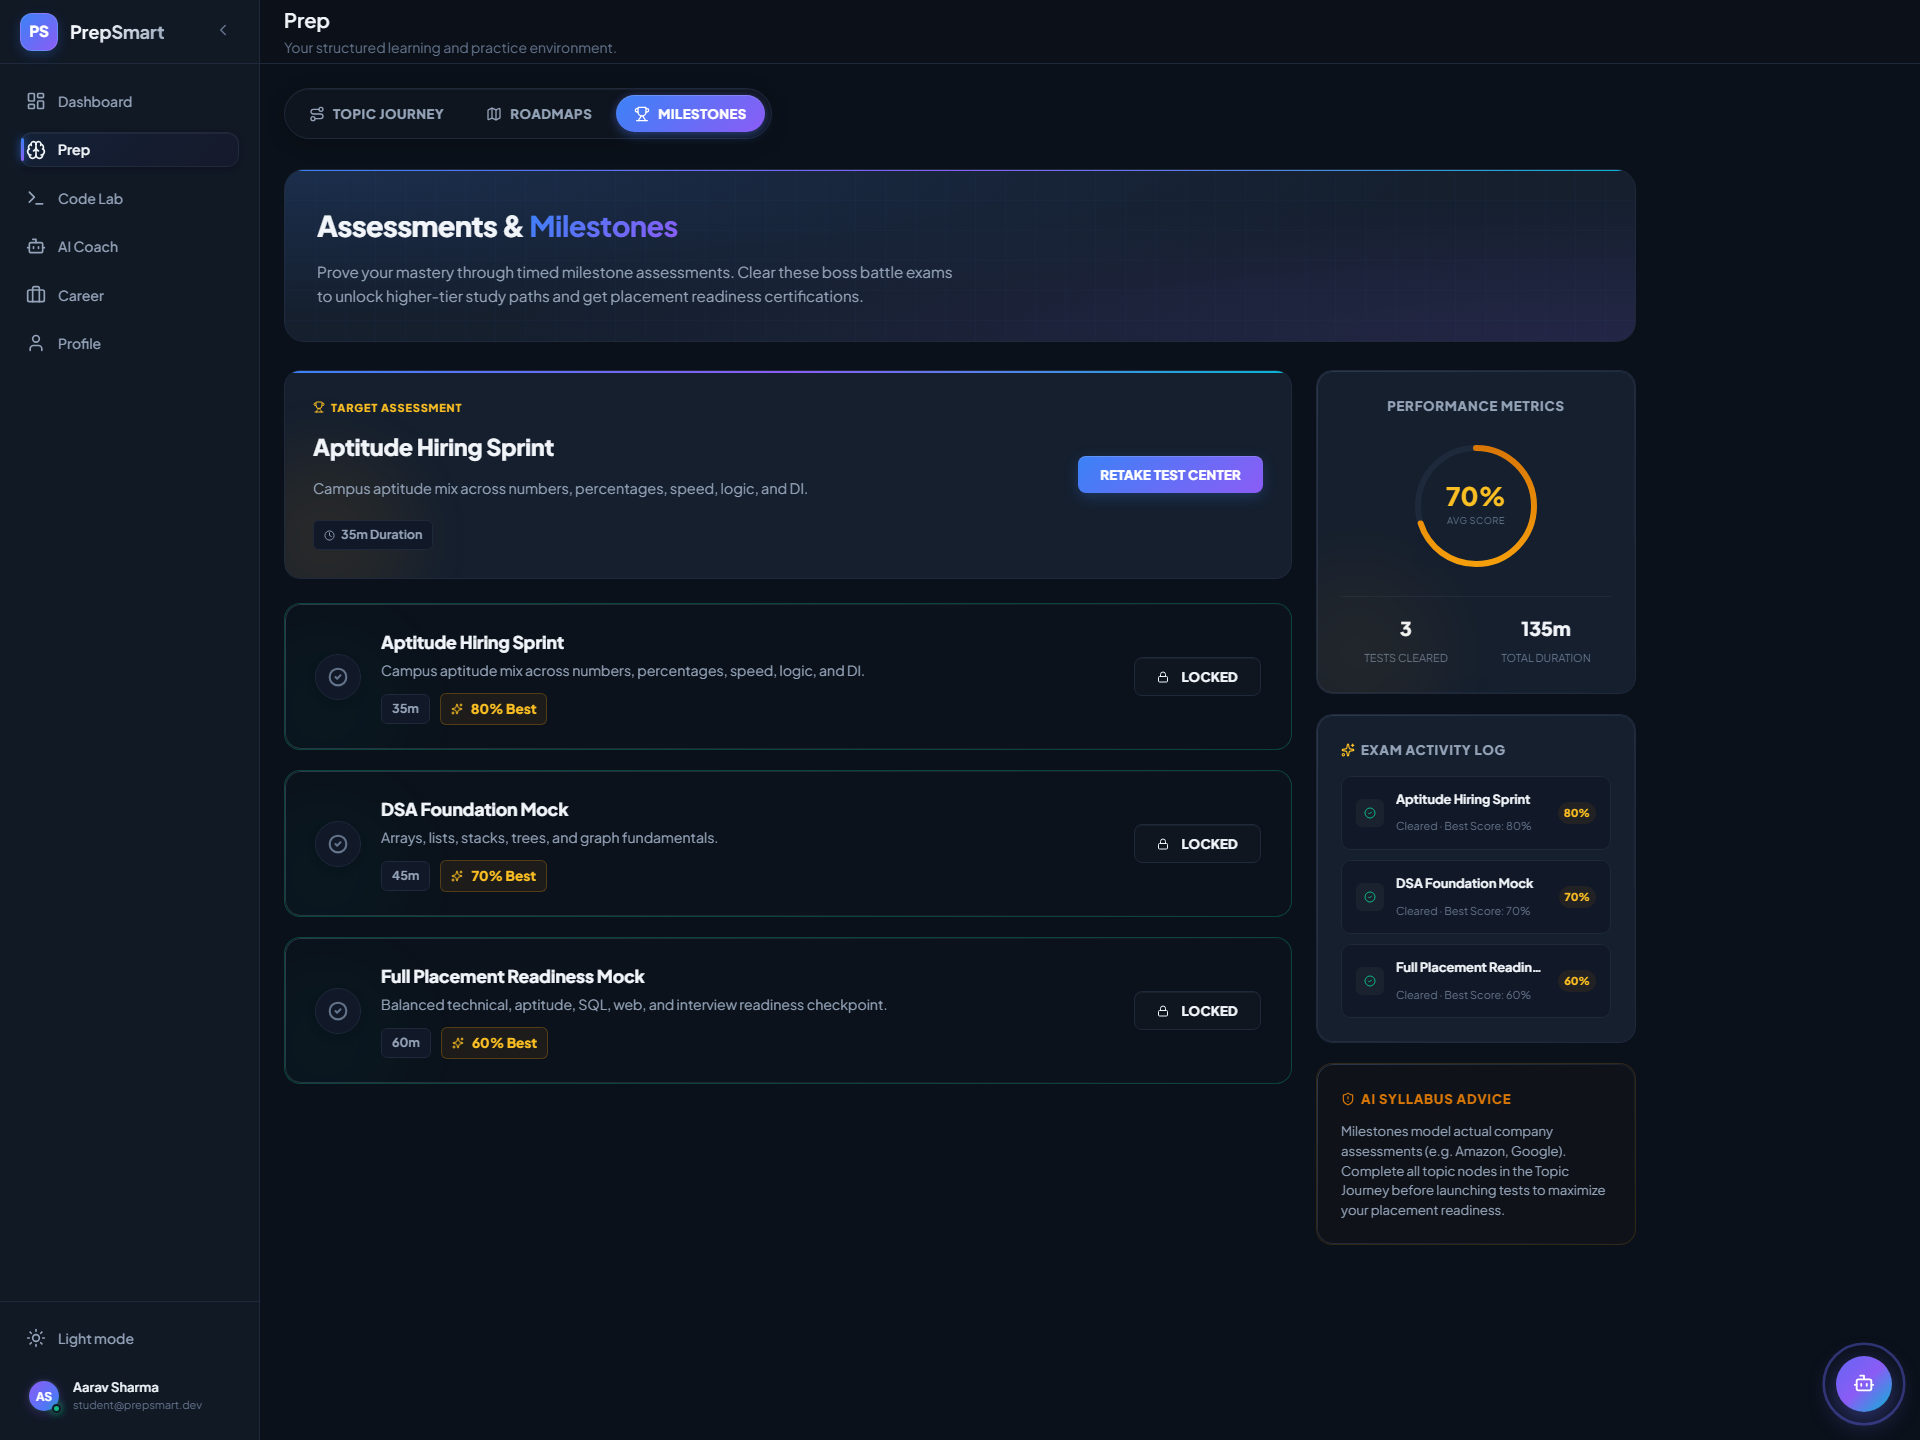
\includegraphics[width=0.95\textwidth]{Media/Chapter 5/milestones.png}
\caption{Learning Milestones}
\label{fig:milestones}
\end{figure}

Figure~\ref{fig:milestones} illustrates the milestone tracking interface. Each milestone represents an important stage within the placement preparation journey and consists of multiple learning activities or assessments.

Students attempt milestone assessments after completing the associated learning topics. The platform records milestone completion status, performance scores, and overall readiness before unlocking subsequent preparation stages.

This structured evaluation approach enables students to monitor their preparation systematically while ensuring that essential concepts are mastered before progressing further.

\subsubsection*{Major Features}

\begin{itemize}

\item Milestone-based assessments.

\item Preparation stage tracking.

\item Automatic progress updates.

\item Learning checkpoint evaluation.

\item Readiness verification.

\item Dashboard integration.

\end{itemize}

\subsection{Topic Study}

The Topic Study interface provides comprehensive learning material for individual subjects included within the placement preparation roadmap. It serves as the primary study environment where students learn theoretical concepts before attempting quizzes, coding exercises, and mock interviews.

\begin{figure}[H]
\centering
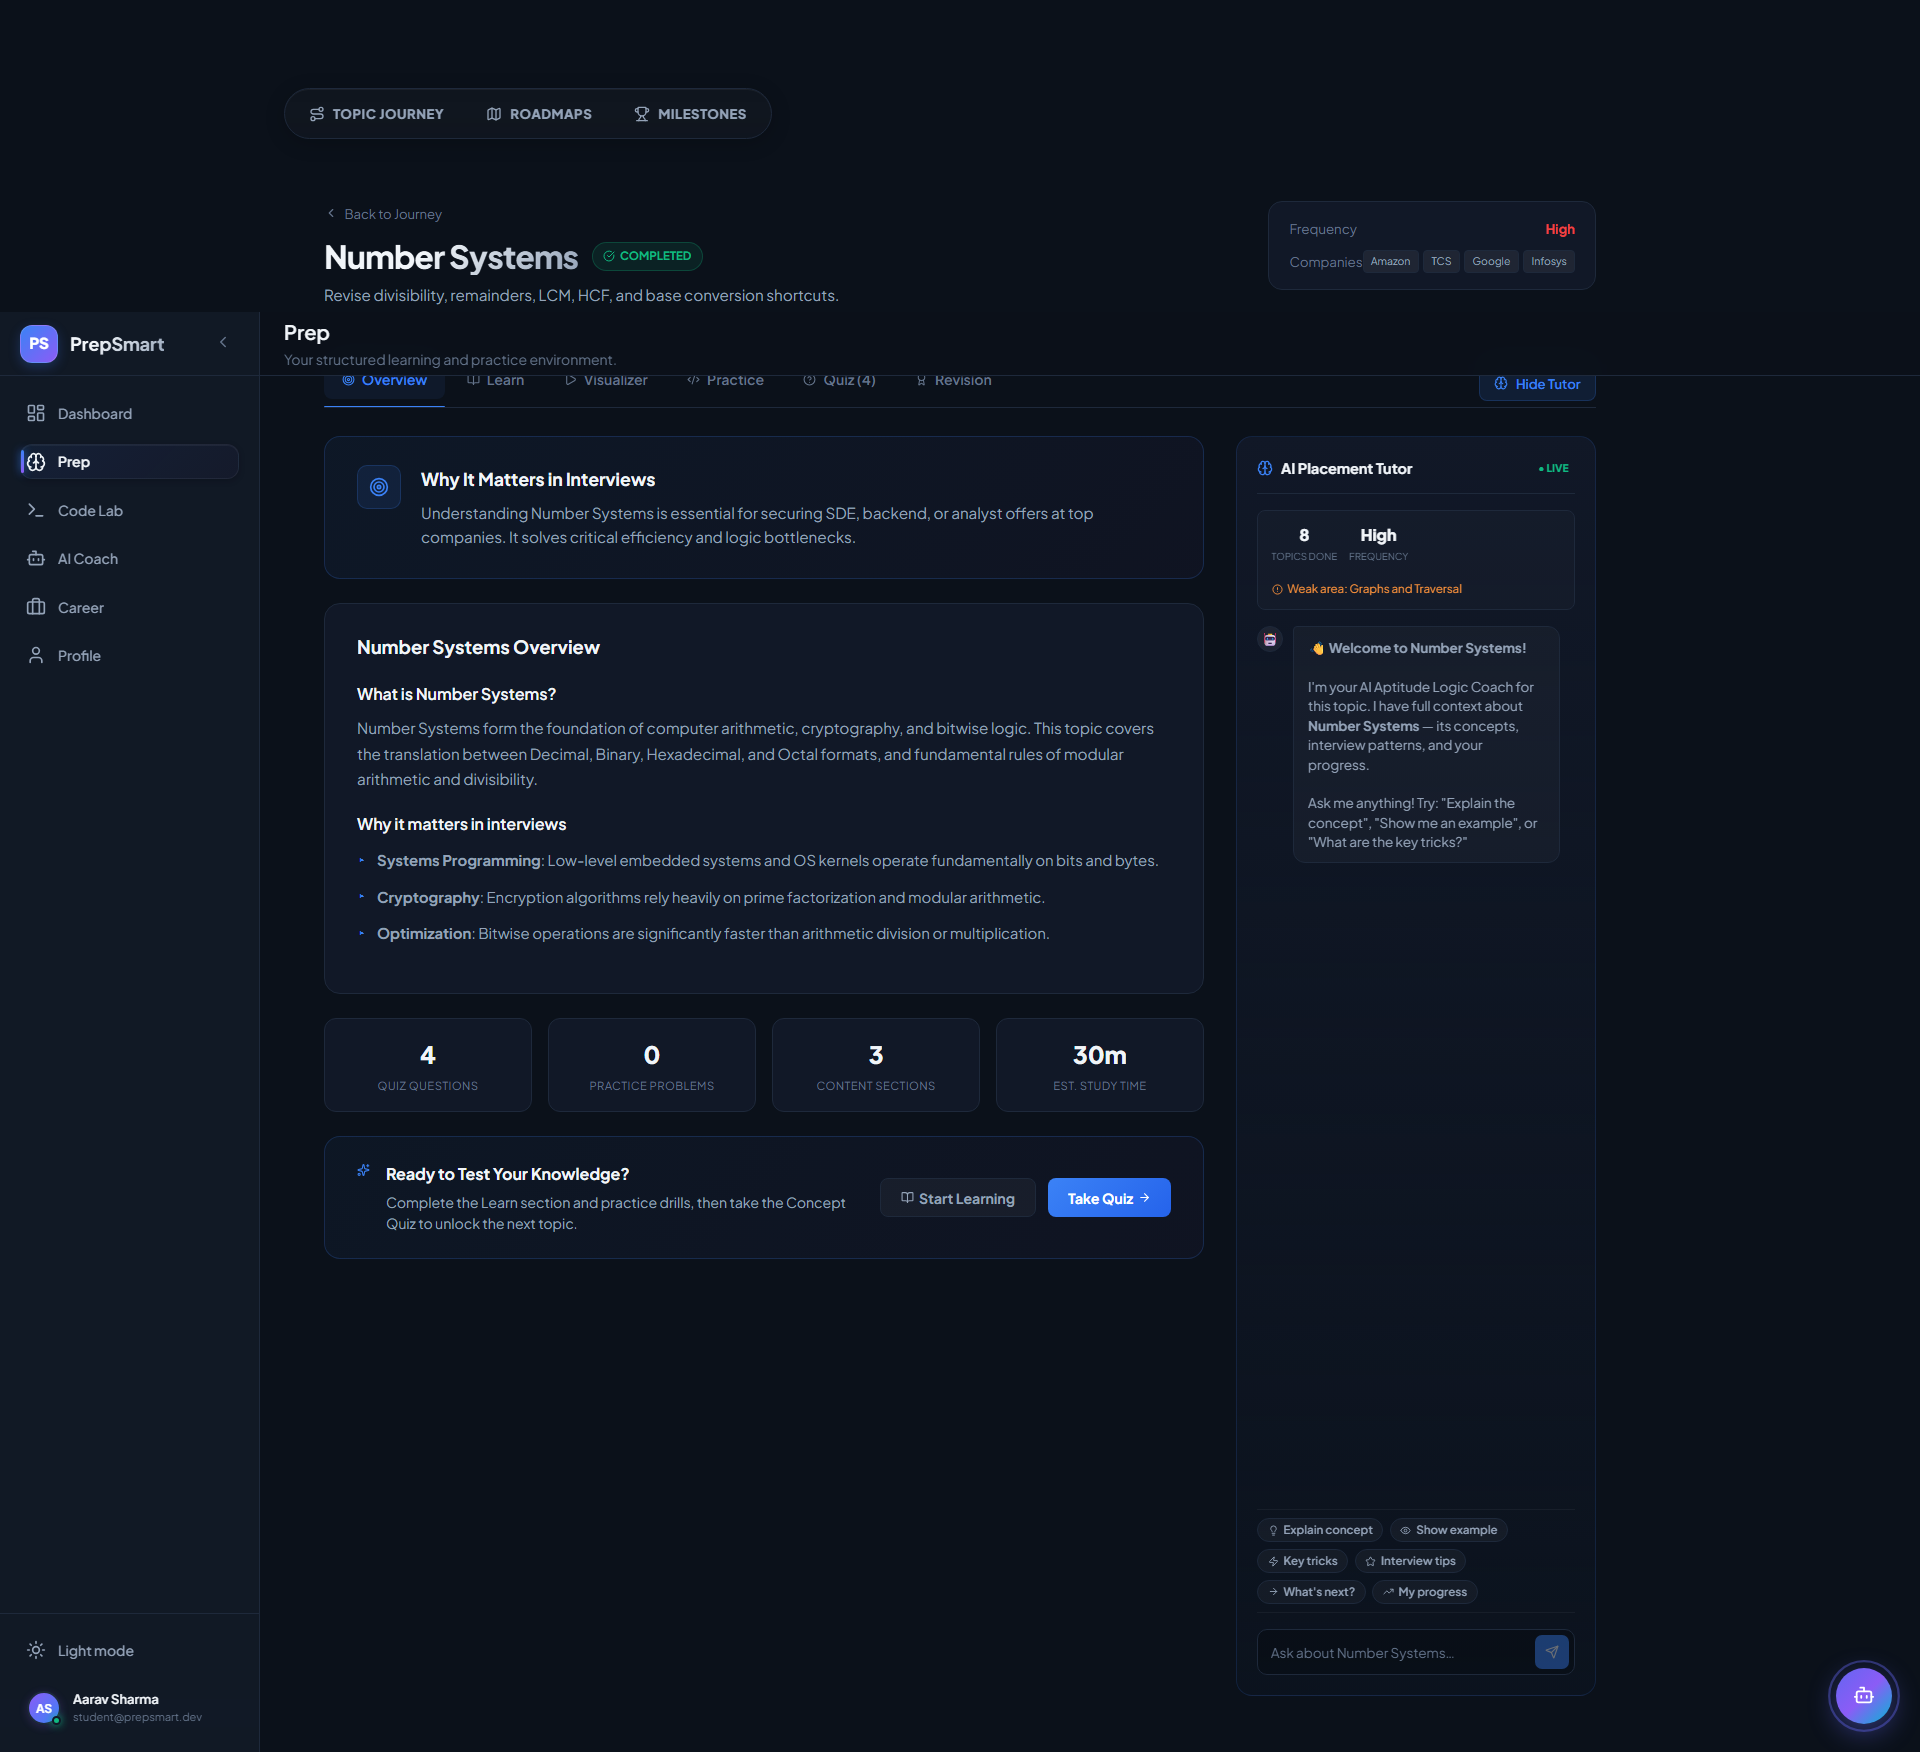
\includegraphics[width=0.95\textwidth]{Media/Chapter 5/topic_study.png}
\caption{Topic Study Interface}
\label{fig:topic_study}
\end{figure}

Figure~\ref{fig:topic_study} presents the Topic Study interface. This page displays detailed learning material, explanations, examples, and related resources for the selected topic.

Students can navigate through different sections of the learning material while monitoring their completion status. After finishing the theoretical content, users can proceed to quizzes, coding practice, or milestone assessments to evaluate their understanding.

The interface combines educational content with progress tracking, enabling students to complete each topic systematically while maintaining consistency throughout their placement preparation journey.

\subsubsection*{Major Features}

\begin{itemize}

\item Topic-wise learning material.

\item Structured educational content.

\item Progress tracking.

\item Easy topic navigation.

\item Integration with quizzes.

\item Direct continuation to coding practice and assessments.

\end{itemize}

\section{Coding Practice Module}

The Coding Practice Module enables students to strengthen their programming skills through an integrated development environment within the PrepSmart platform. Instead of switching between multiple coding websites, students can solve programming problems, execute programs, participate in coding contests, and monitor their coding performance using a unified interface.

The module consists of four major interfaces: Problem Arena, Coding Workspace, Standalone Code Workspace, and Contest Hub. These interfaces collectively provide an interview-oriented programming environment that closely resembles modern online coding assessment platforms.

\subsection{Problem Arena}

The Problem Arena serves as the central repository of programming problems available within PrepSmart. It allows students to browse coding questions of varying difficulty levels and practice problems according to their preparation requirements.

\begin{figure}[H]
\centering
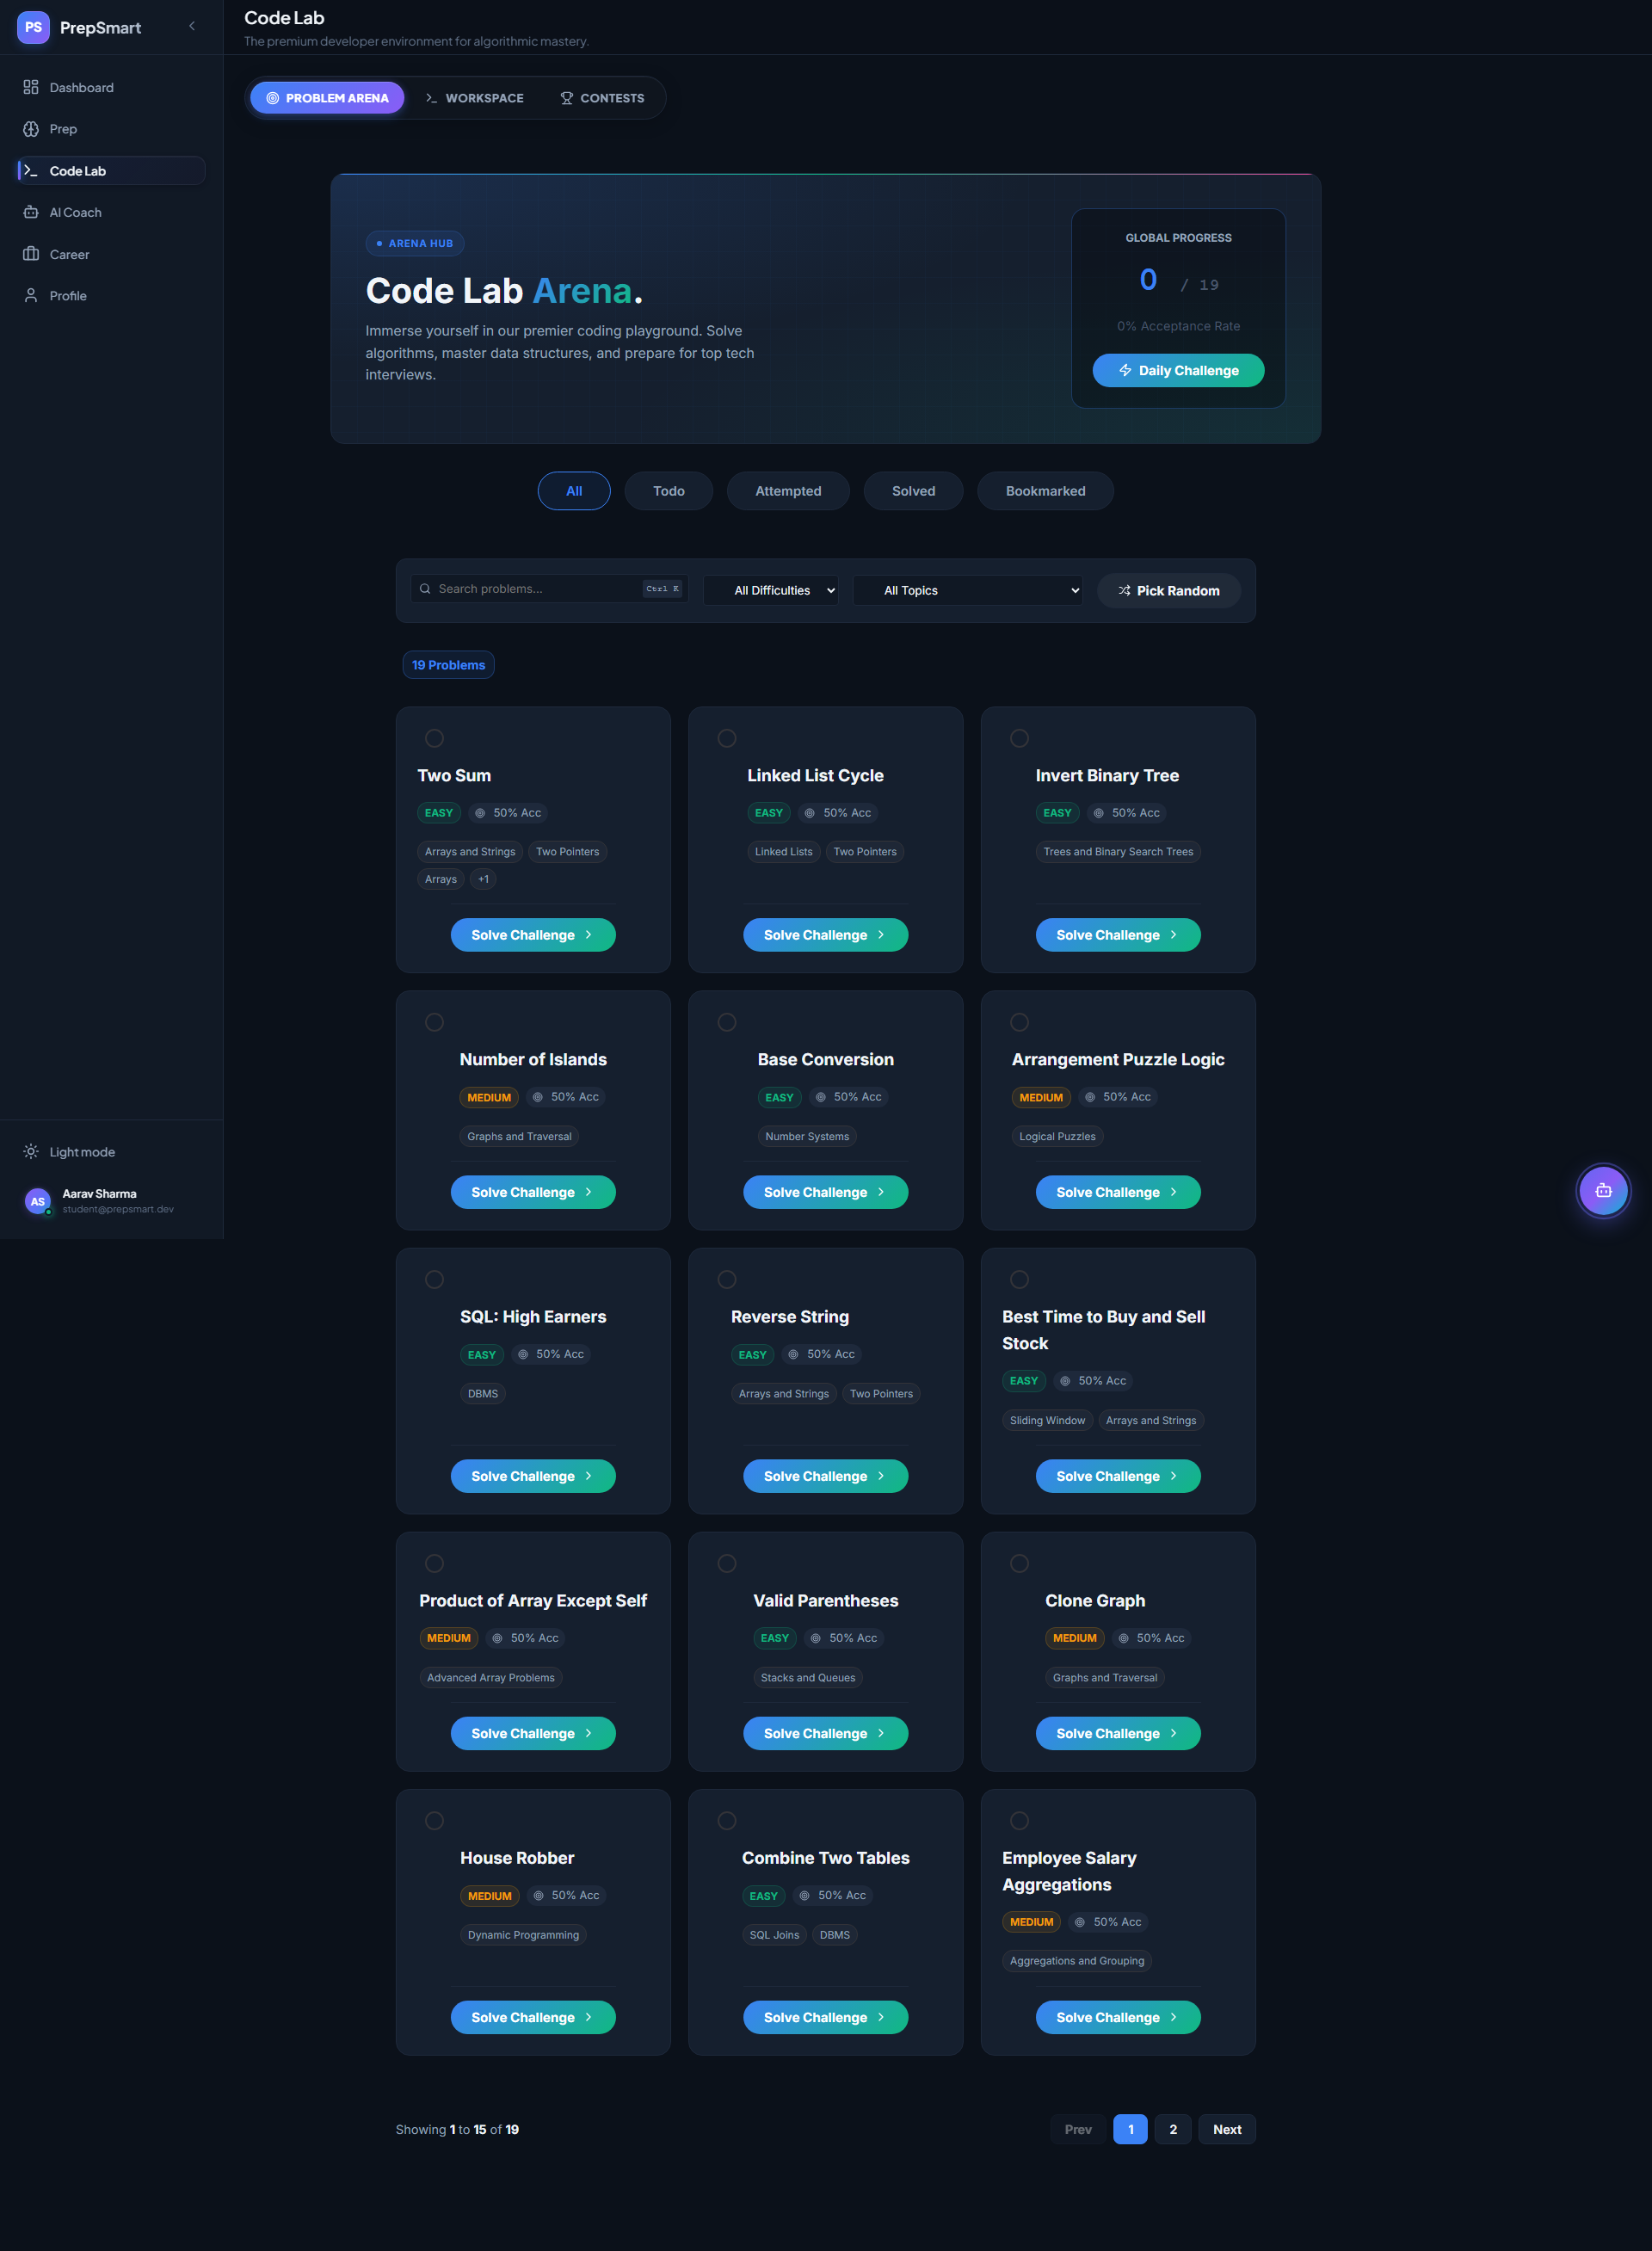
\includegraphics[width=0.95\textwidth]{Media/Chapter 5/problem_arena.png}
\caption{Problem Arena}
\label{fig:problem_arena}
\end{figure}

Figure~\ref{fig:problem_arena} illustrates the Problem Arena interface. This page displays the collection of programming problems available for practice. Students can browse problems based on difficulty level, topic, or interview relevance.

Each programming problem includes a title, difficulty level, associated topics, company tags, and other important information required before attempting the solution. The organized presentation allows students to efficiently select suitable problems according to their current preparation level.

The Problem Arena acts as the entry point to the coding environment and provides easy navigation to the coding workspace for solving selected problems.

\subsubsection*{Major Features}

\begin{itemize}

\item Collection of programming problems.

\item Difficulty-based problem categorization.

\item Topic-wise organization.

\item Company-specific problem tags.

\item Easy problem search and navigation.

\item Direct access to the coding workspace.

\end{itemize}

\subsection{Coding Workspace}

The Coding Workspace provides an integrated programming environment where students can write, execute, debug, and submit programming solutions. It closely simulates the coding environments commonly used during online placement assessments.

\begin{figure}[H]
\centering
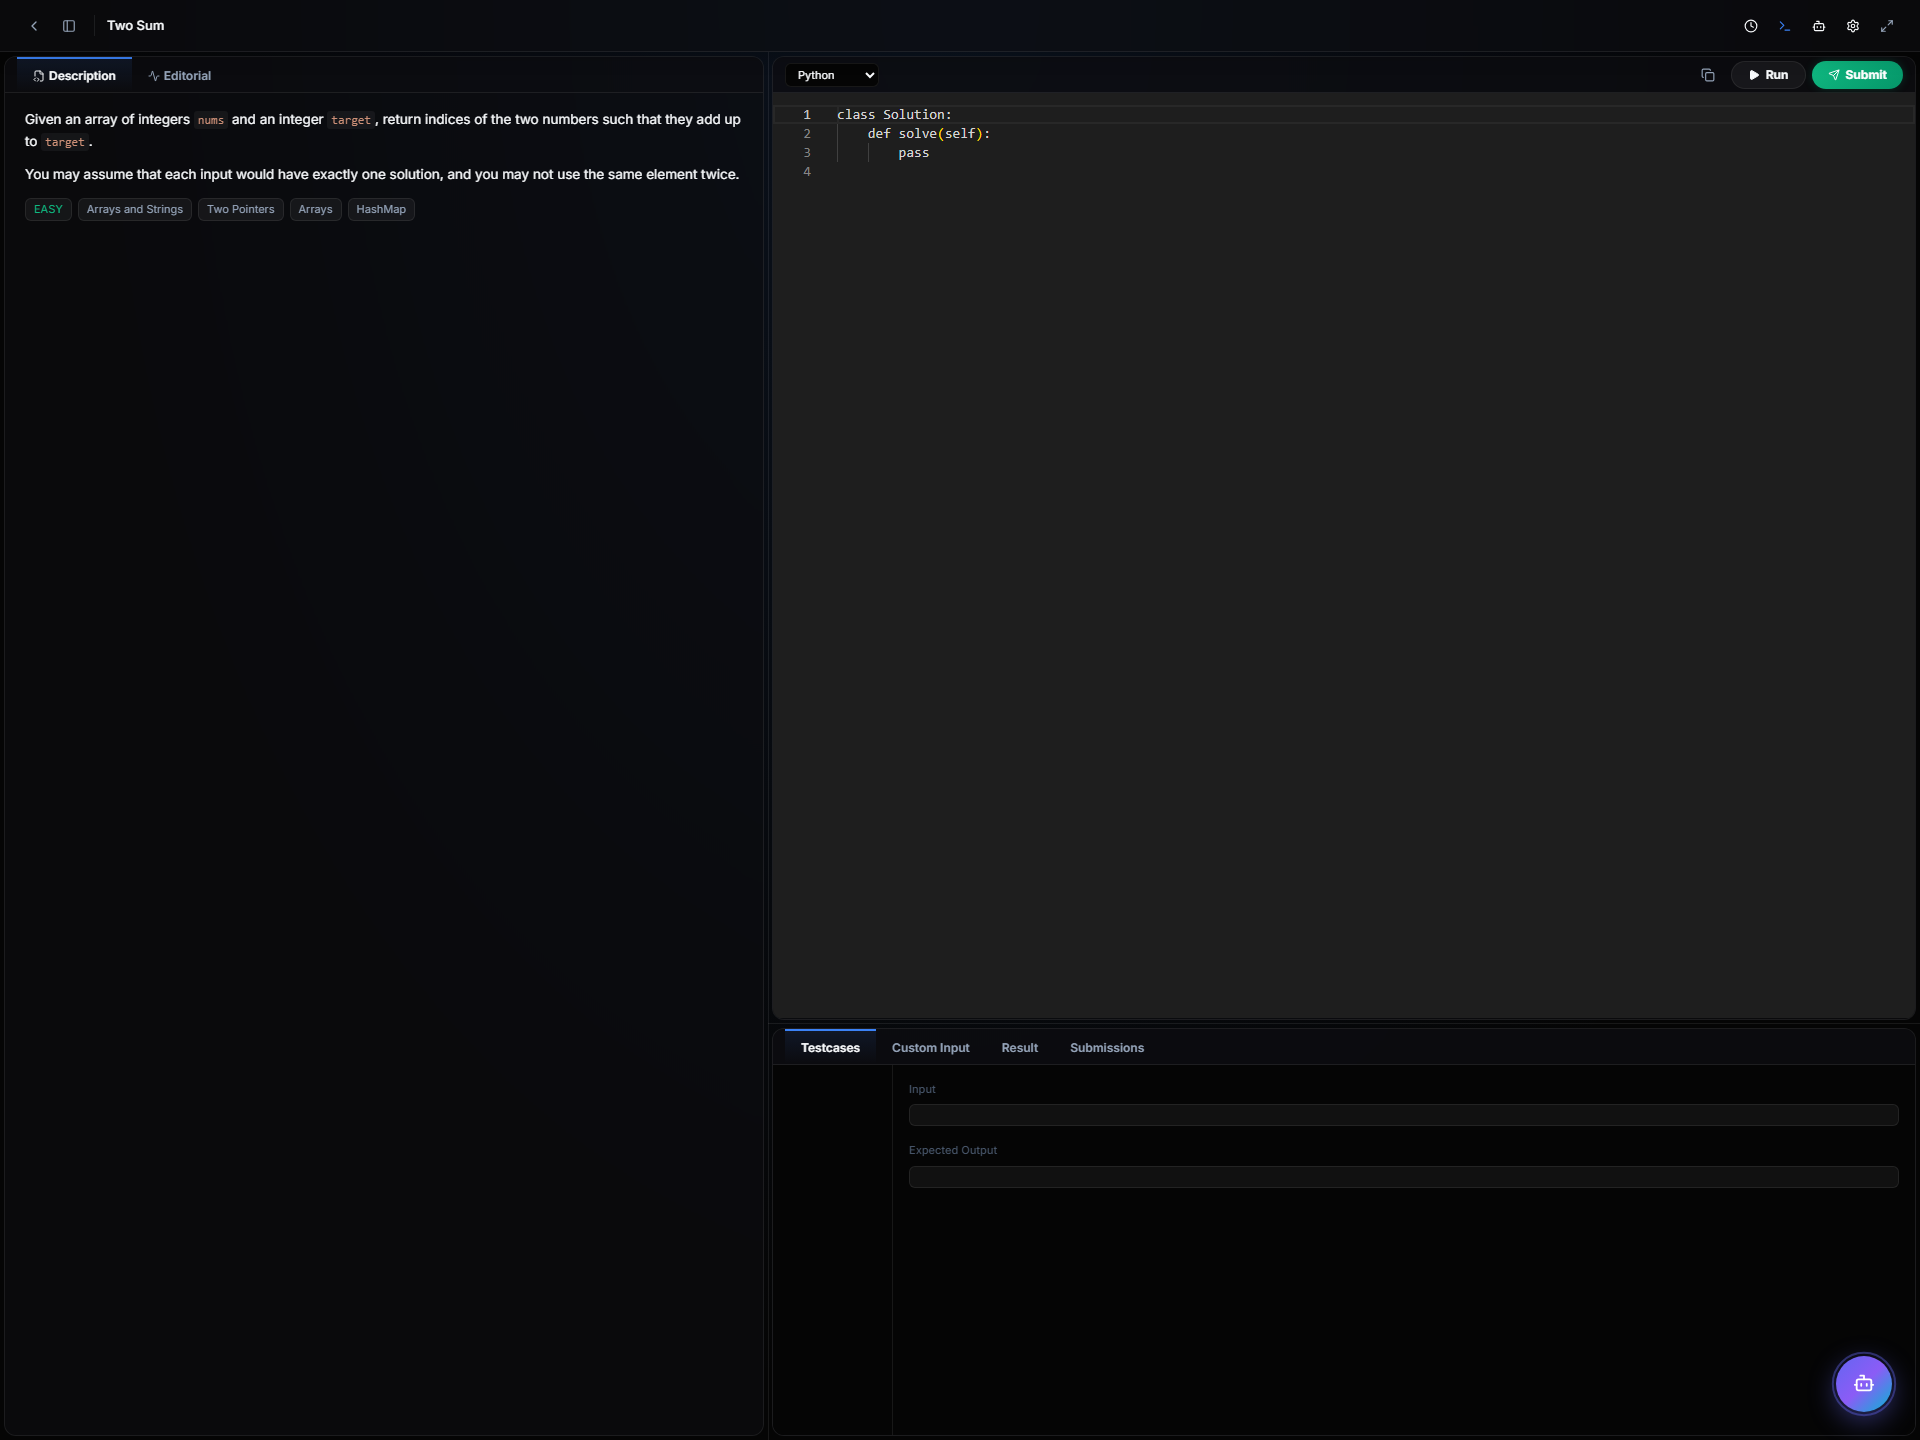
\includegraphics[width=0.95\textwidth]{Media/Chapter 5/coding_workspace.png}
\caption{Coding Workspace}
\label{fig:coding_workspace}
\end{figure}

Figure~\ref{fig:coding_workspace} presents the Coding Workspace of PrepSmart. The interface combines the problem statement, source code editor, programming language selection, custom input, execution controls, and output console within a single screen.

Students can write solutions using the integrated editor, execute programs with custom inputs, and verify the generated output before final submission. The platform also reports execution statistics such as runtime, execution status, and error messages, enabling students to debug their programs efficiently.

The integrated design minimizes distractions by providing all programming resources within a unified coding environment.

\subsubsection*{Major Features}

\begin{itemize}

\item Integrated source code editor.

\item Programming language selection.

\item Custom input execution.

\item Output console.

\item Runtime and error reporting.

\item Program submission facility.

\end{itemize}

\subsection{Standalone Code Workspace}

The Standalone Code Workspace enables students to write and execute programs independently without selecting a predefined coding problem. This interface is useful for experimenting with programming concepts, debugging code, and practicing algorithms freely.

\begin{figure}[H]
\centering
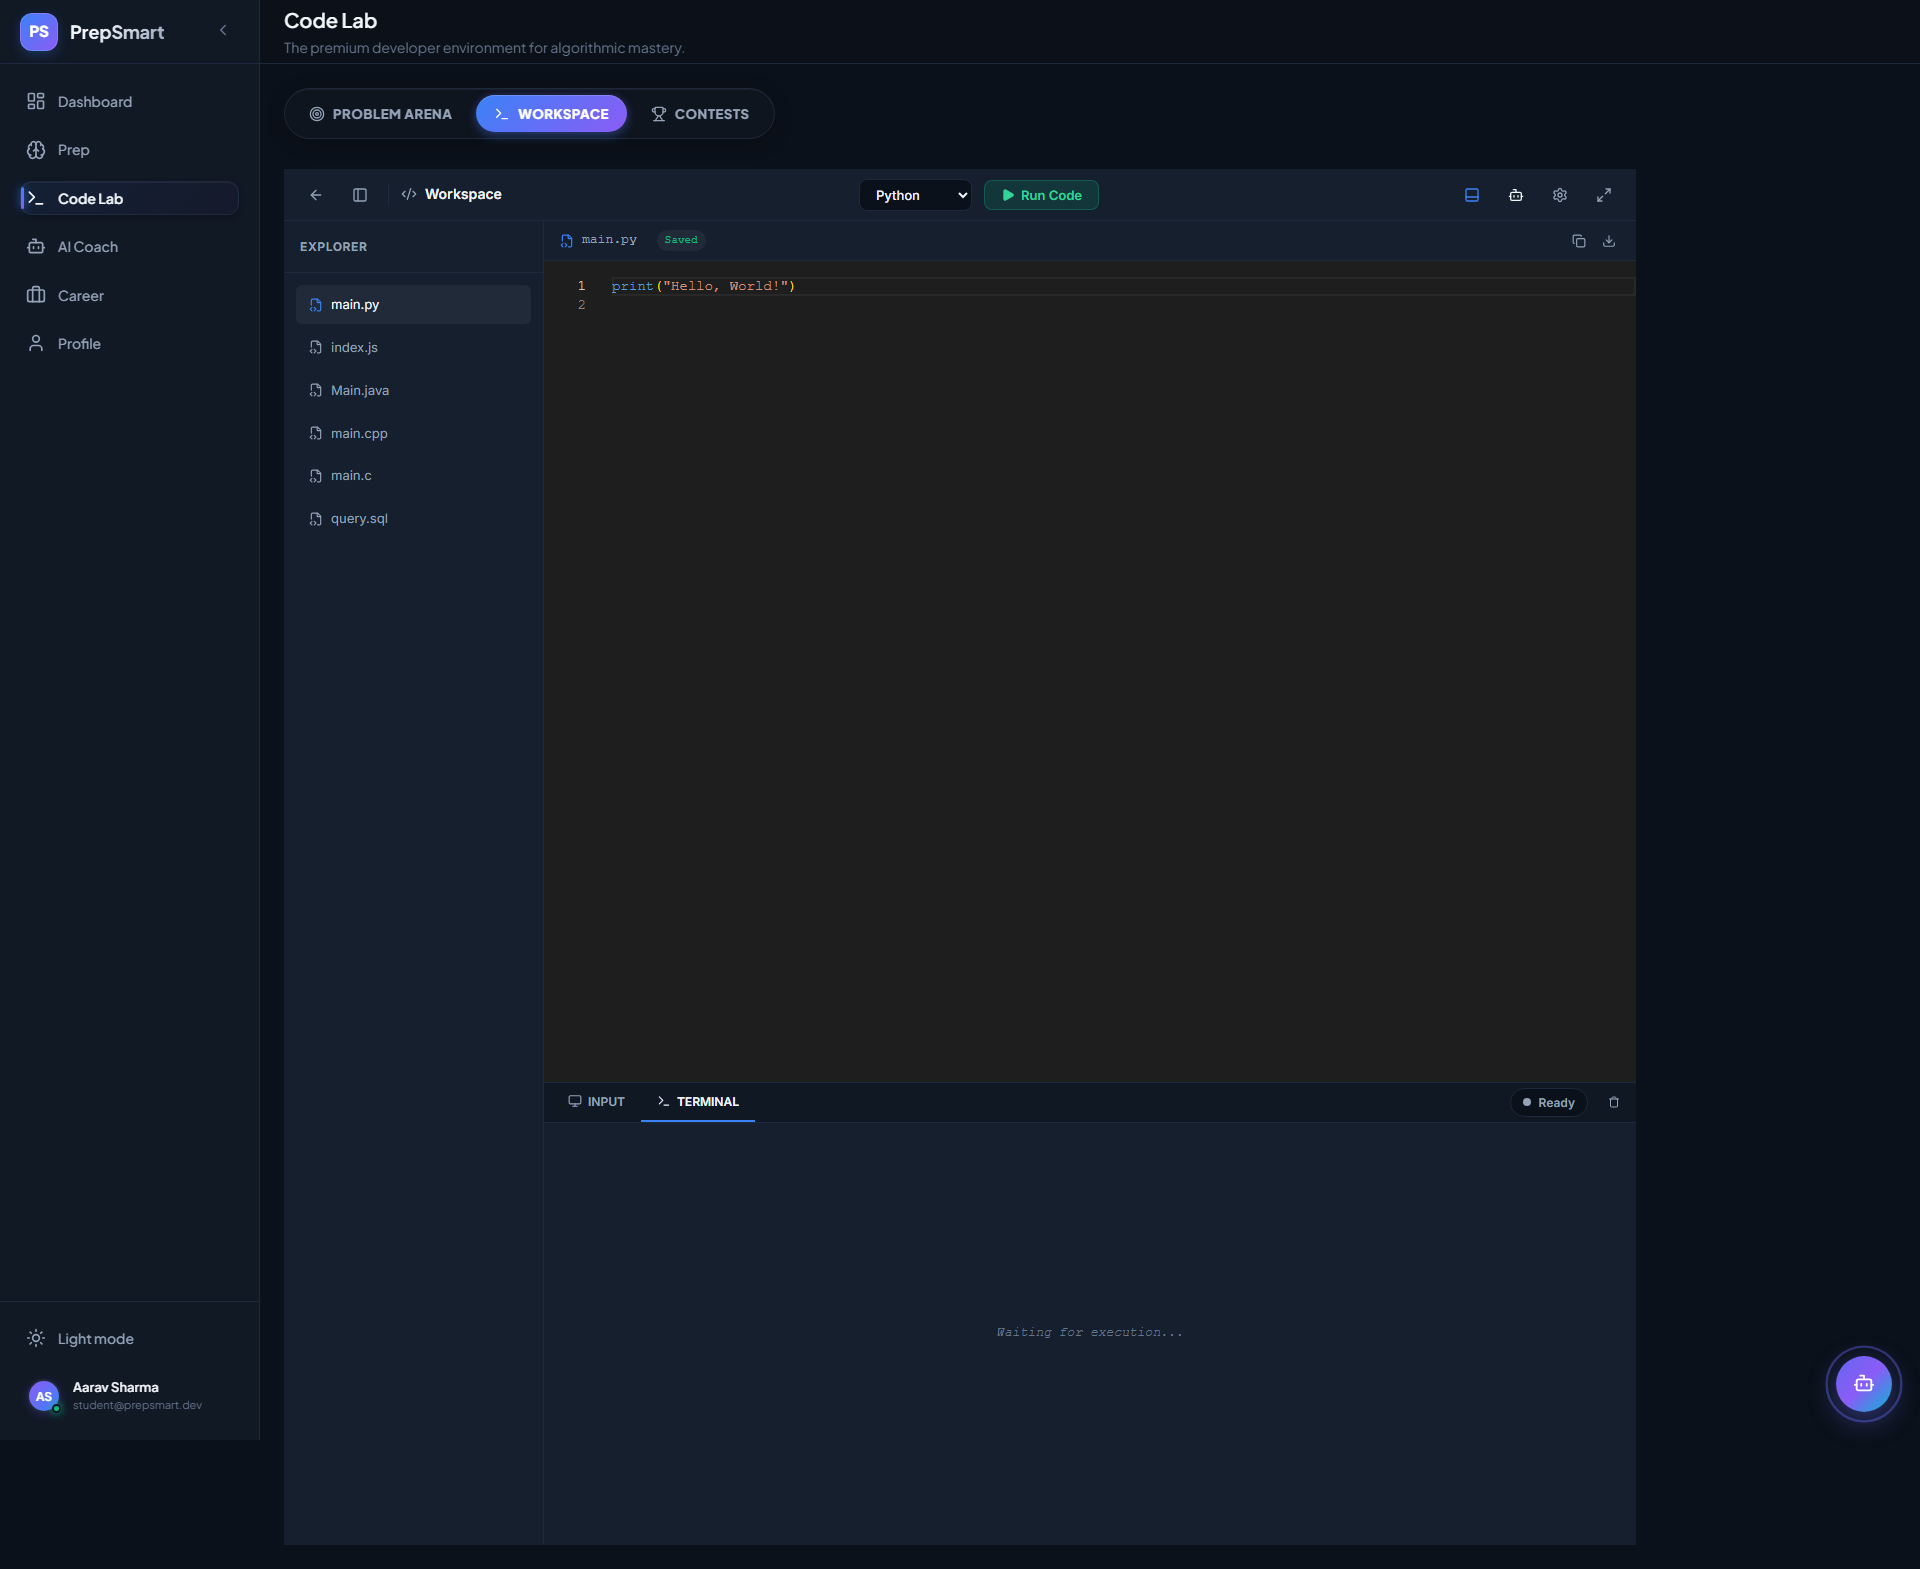
\includegraphics[width=0.95\textwidth]{Media/Chapter 5/standalone_workspace.png}
\caption{Standalone Code Workspace}
\label{fig:standalone_workspace}
\end{figure}

Figure~\ref{fig:standalone_workspace} illustrates the Standalone Code Workspace. Unlike the problem-specific coding environment, this workspace allows students to develop and execute programs without predefined constraints or evaluation criteria.

The interface provides a programming editor, language selection, execution controls, and an output console. Students can use this environment for experimenting with programming techniques, verifying algorithm implementations, or practicing coding concepts before attempting formal programming challenges.

\subsubsection*{Major Features}

\begin{itemize}

\item Independent programming environment.

\item Custom code execution.

\item Multi-language support.

\item Output visualization.

\item Algorithm experimentation.

\item Debugging assistance.

\end{itemize}

\subsection{Contest Hub}

The Contest Hub provides students with information about ongoing and upcoming programming contests from multiple competitive coding platforms. It encourages students to participate in real-world programming competitions and improve their problem-solving abilities.

\begin{figure}[H]
\centering
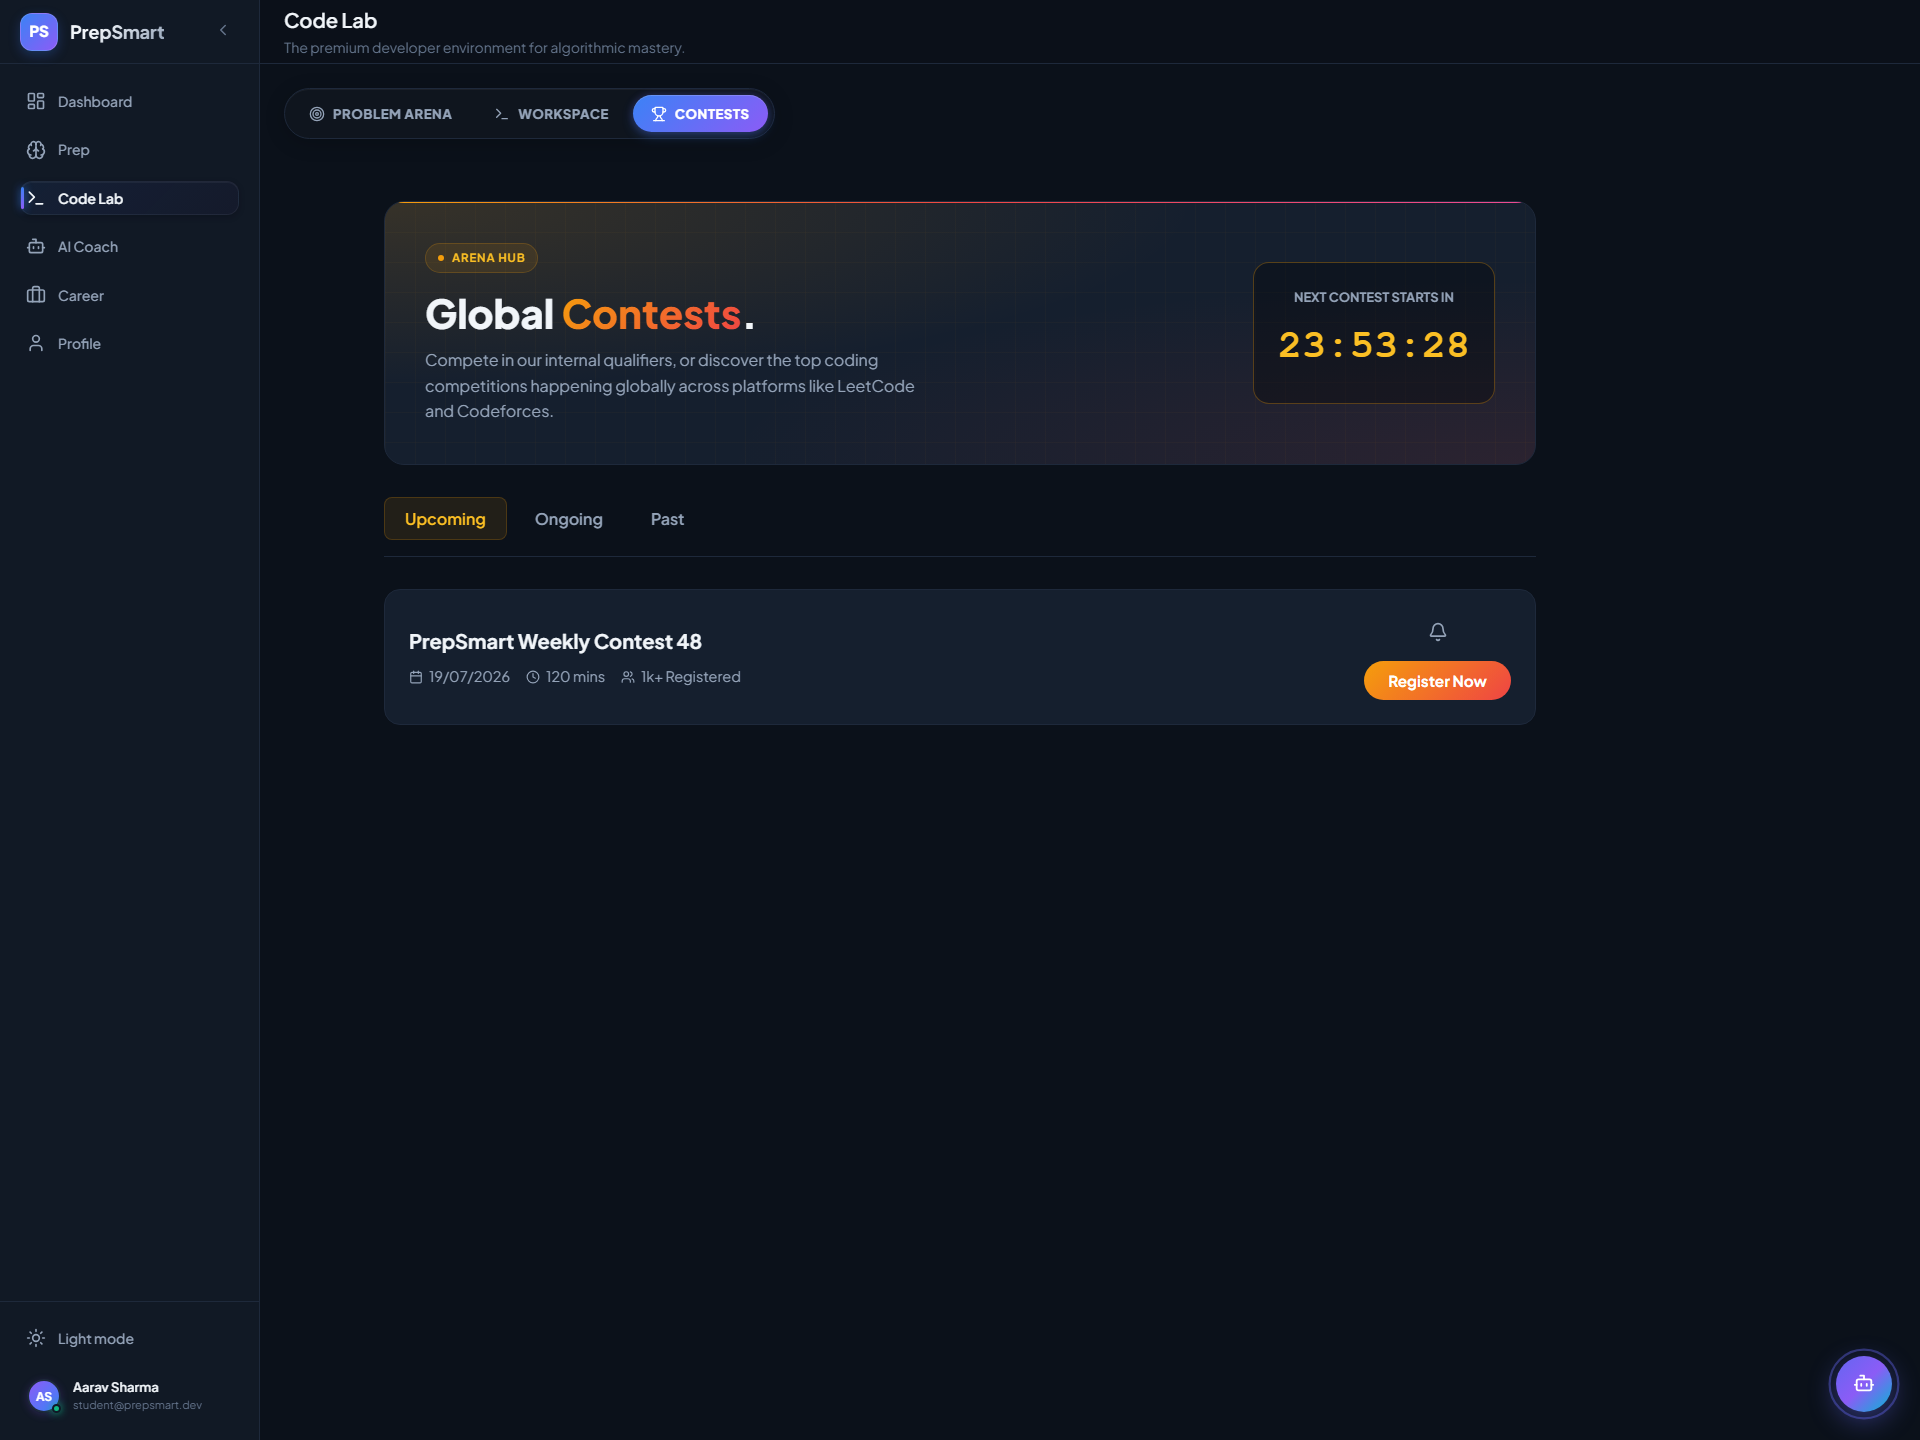
\includegraphics[width=0.95\textwidth]{Media/Chapter 5/contest_hub.png}
\caption{Contest Hub}
\label{fig:contest_hub}
\end{figure}

Figure~\ref{fig:contest_hub} presents the Contest Hub interface of PrepSmart. The page displays programming contests collected from external coding platforms and presents information such as contest names, start times, durations, hosting platforms, and registration links.

Students can easily browse upcoming contests and participate directly from the platform. The centralized presentation of contest information eliminates the need to visit multiple coding websites individually and encourages continuous participation in competitive programming activities.

\subsubsection*{Major Features}

\begin{itemize}

\item Display of upcoming coding contests.

\item Contest platform information.

\item Contest schedules.

\item Registration links.

\item Integration with external contest providers.

\item Encouragement for competitive programming.

\end{itemize}

\section{AI Interview Module}

The AI Interview Module provides students with an interactive interview preparation environment that simulates technical interviews using Artificial Intelligence. Unlike conventional interview preparation methods, this module enables students to answer technical questions, receive automated feedback, and evaluate their interview readiness within the PrepSmart platform.

The interface is designed to improve communication skills, technical understanding, and confidence by providing a realistic interview experience. Students can practice repeatedly while monitoring their improvement over time.

\begin{figure}[H]
\centering
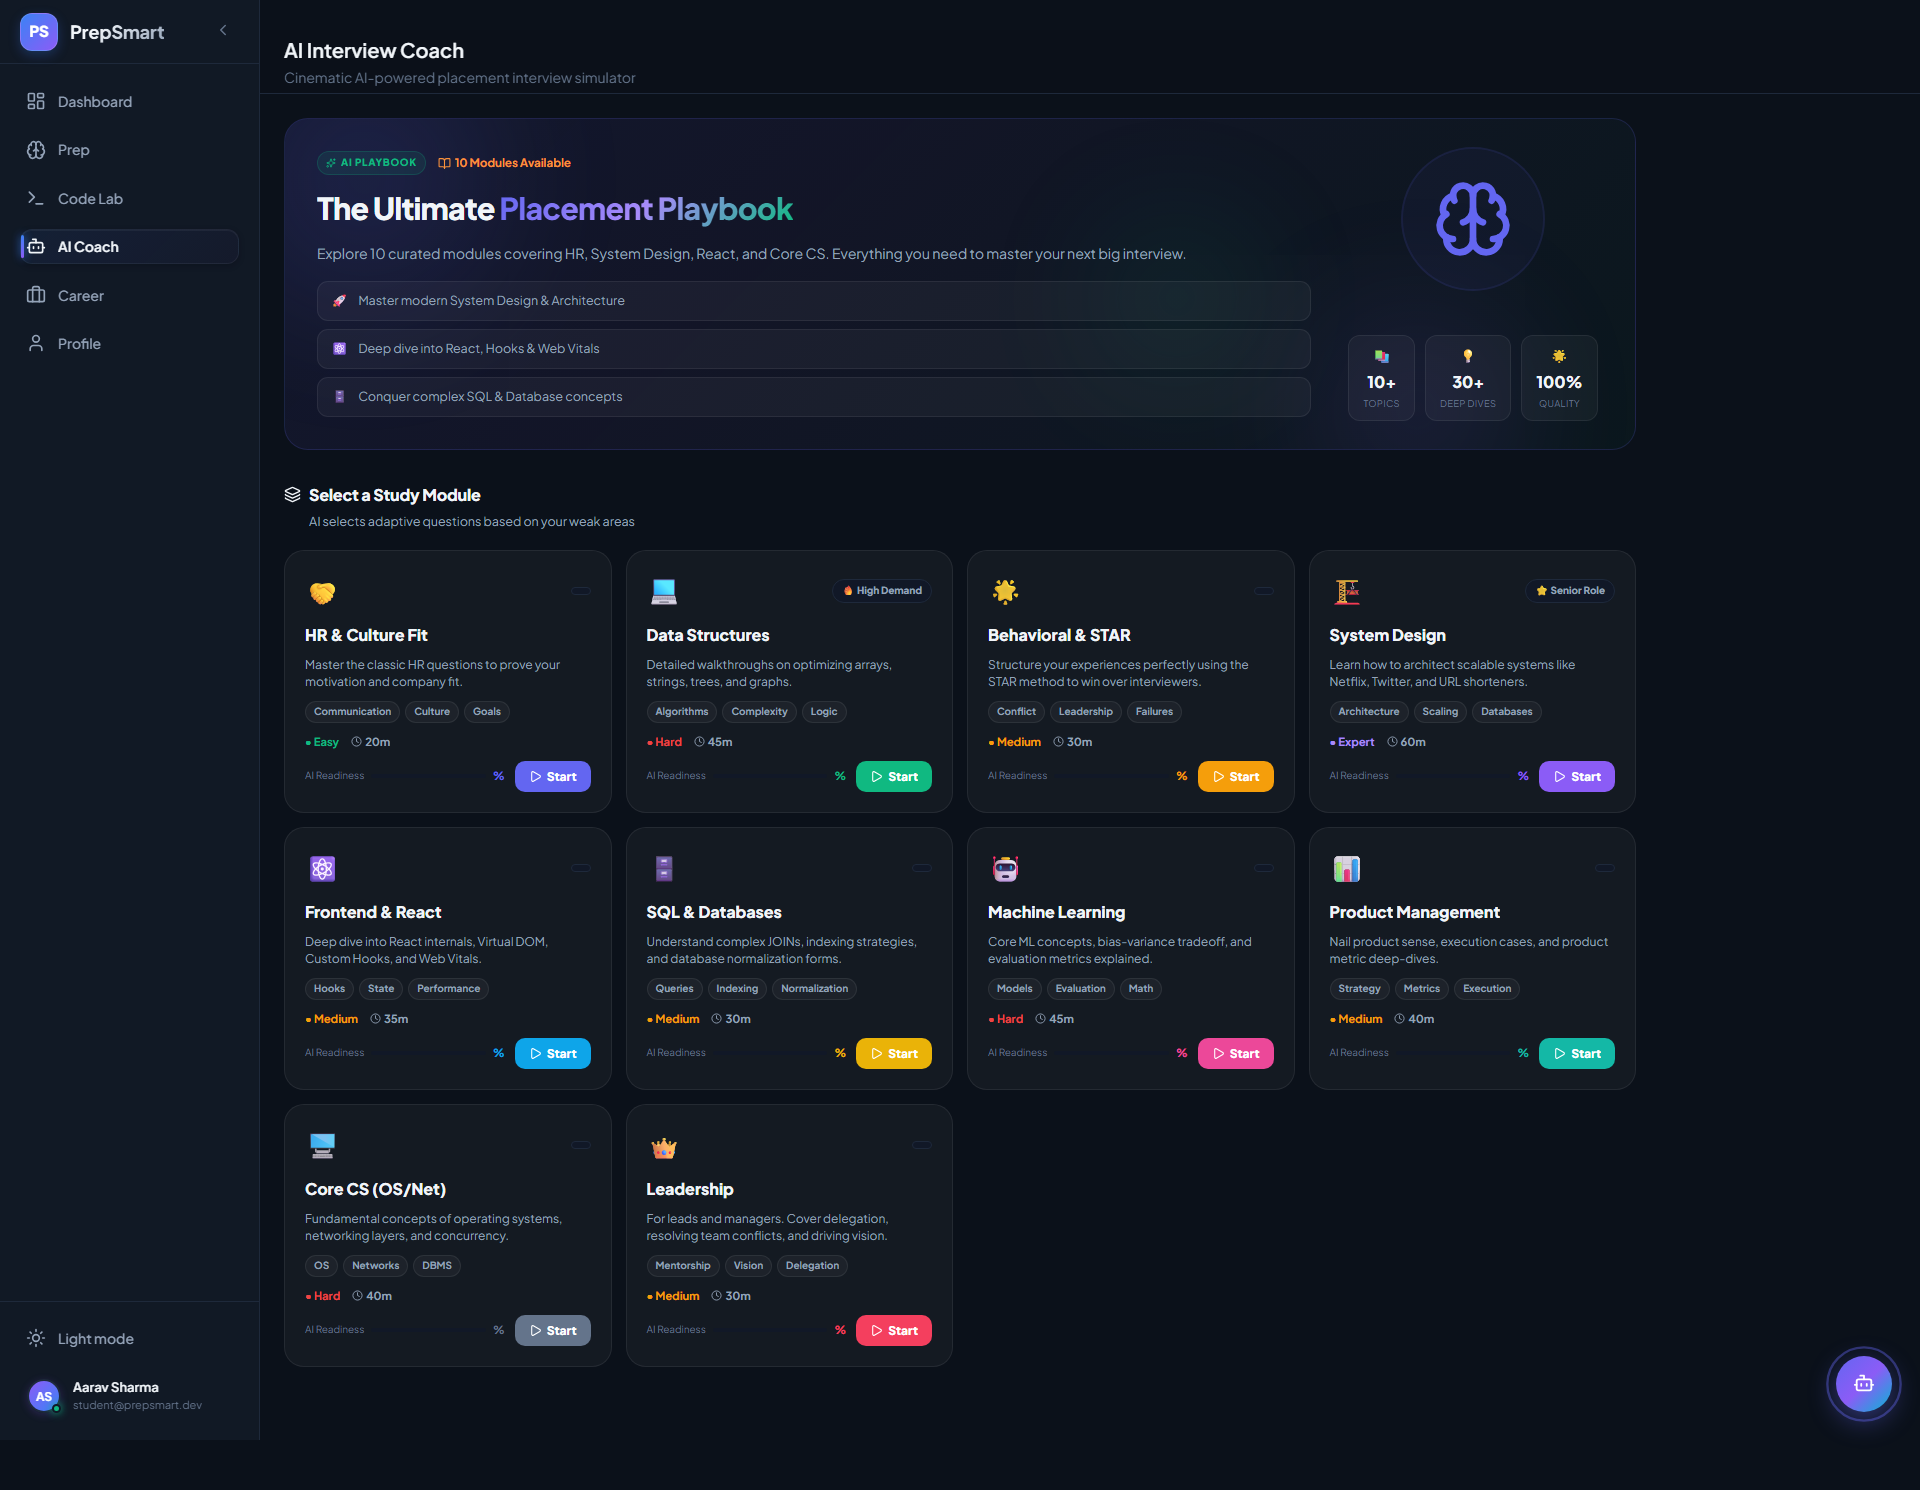
\includegraphics[width=0.95\textwidth]{Media/Chapter 5/ai_interview.png}
\caption{AI Interview Interface}
\label{fig:ai_interview}
\end{figure}

Figure~\ref{fig:ai_interview} illustrates the AI Interview interface of PrepSmart. The page allows students to participate in simulated interview sessions by selecting interview categories and answering technical questions presented by the system.

During an interview session, each response submitted by the student is evaluated by the backend, and AI-generated feedback is provided to highlight strengths, weaknesses, and possible improvements. The interface also maintains interview progress and displays evaluation results in an organized manner.

By providing immediate feedback and realistic interview practice, the module enables students to strengthen both technical knowledge and communication skills before attending actual placement interviews.

\subsection*{Major Features}

\begin{itemize}

\item AI-assisted interview simulation.

\item Technical question evaluation.

\item Automated feedback generation.

\item Interview progress tracking.

\item Performance scoring.

\item Interview history management.

\end{itemize}

\section{Company Preparation Module}

The Company Preparation Module enables students to prepare specifically for companies participating in campus recruitment. Instead of following a general preparation strategy, students can explore company-specific requirements, monitor their readiness, and identify the topics that require further improvement.

The module provides separate interfaces for viewing available companies and detailed preparation information for each selected company.

\subsection{Companies}

The Companies interface displays the list of organizations available within the PrepSmart platform. Students can browse companies and select the organization for which they wish to evaluate their preparation.

\begin{figure}[H]
\centering
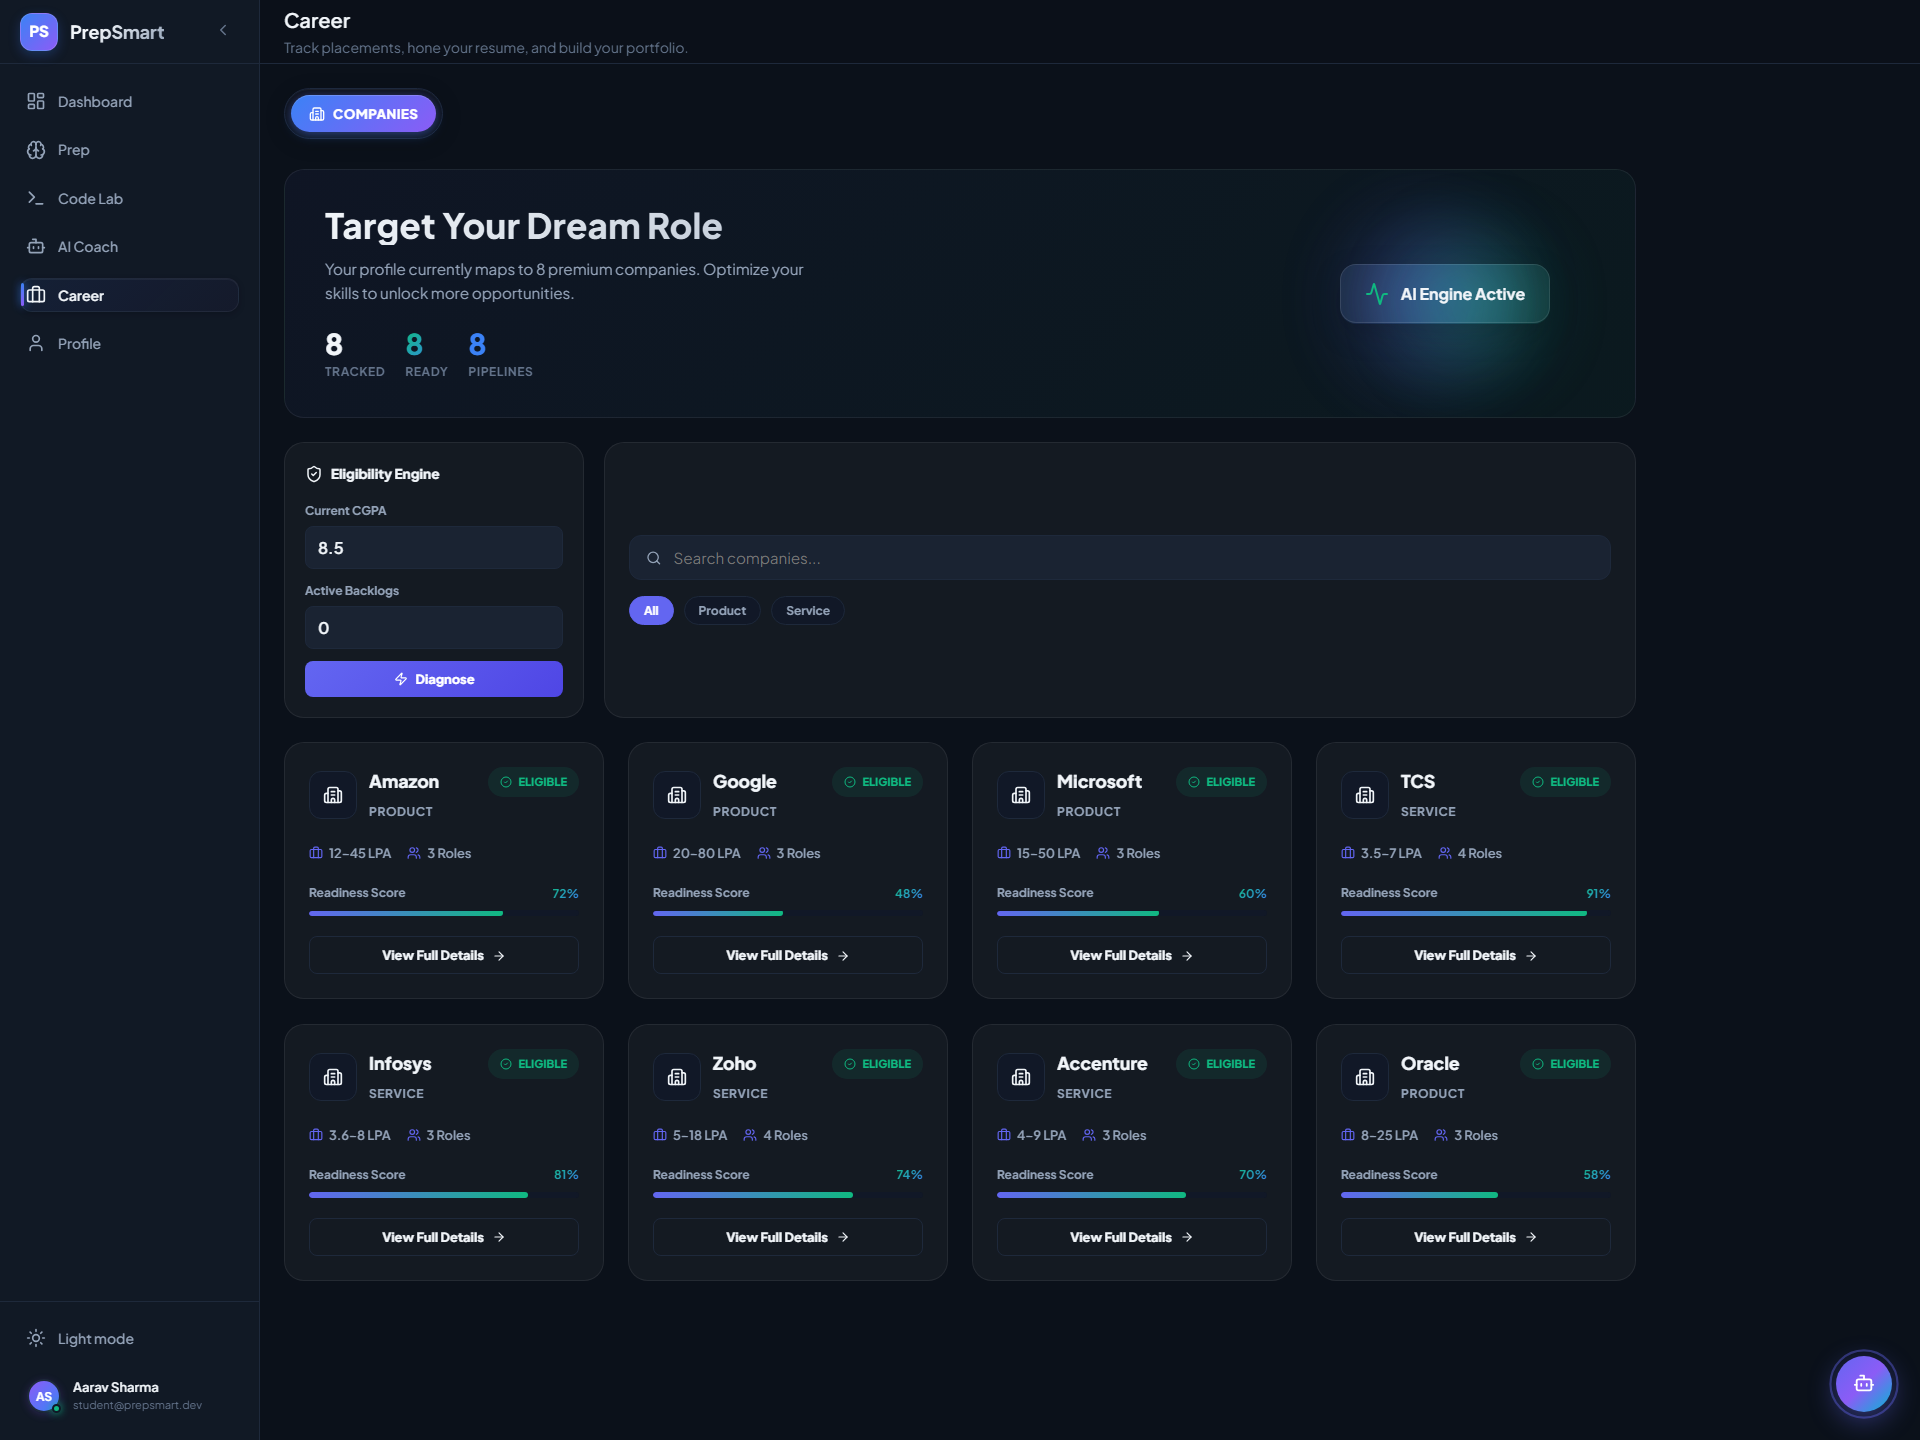
\includegraphics[width=0.95\textwidth]{Media/Chapter 5/companies.png}
\caption{Companies Interface}
\label{fig:companies}
\end{figure}

Figure~\ref{fig:companies} presents the Companies interface of PrepSmart. The page provides an organized list of target companies together with essential preparation information. Students can browse available organizations and select a company to view detailed preparation requirements.

The interface acts as the starting point for company-specific preparation and provides quick navigation to detailed readiness information.

\subsubsection*{Major Features}

\begin{itemize}

\item List of target companies.

\item Company search.

\item Company selection.

\item Quick navigation.

\item Preparation overview.

\end{itemize}

\subsection{Company Details}

The Company Details interface provides comprehensive information regarding the selected company's preparation requirements and the student's readiness status.

\begin{figure}[H]
\centering
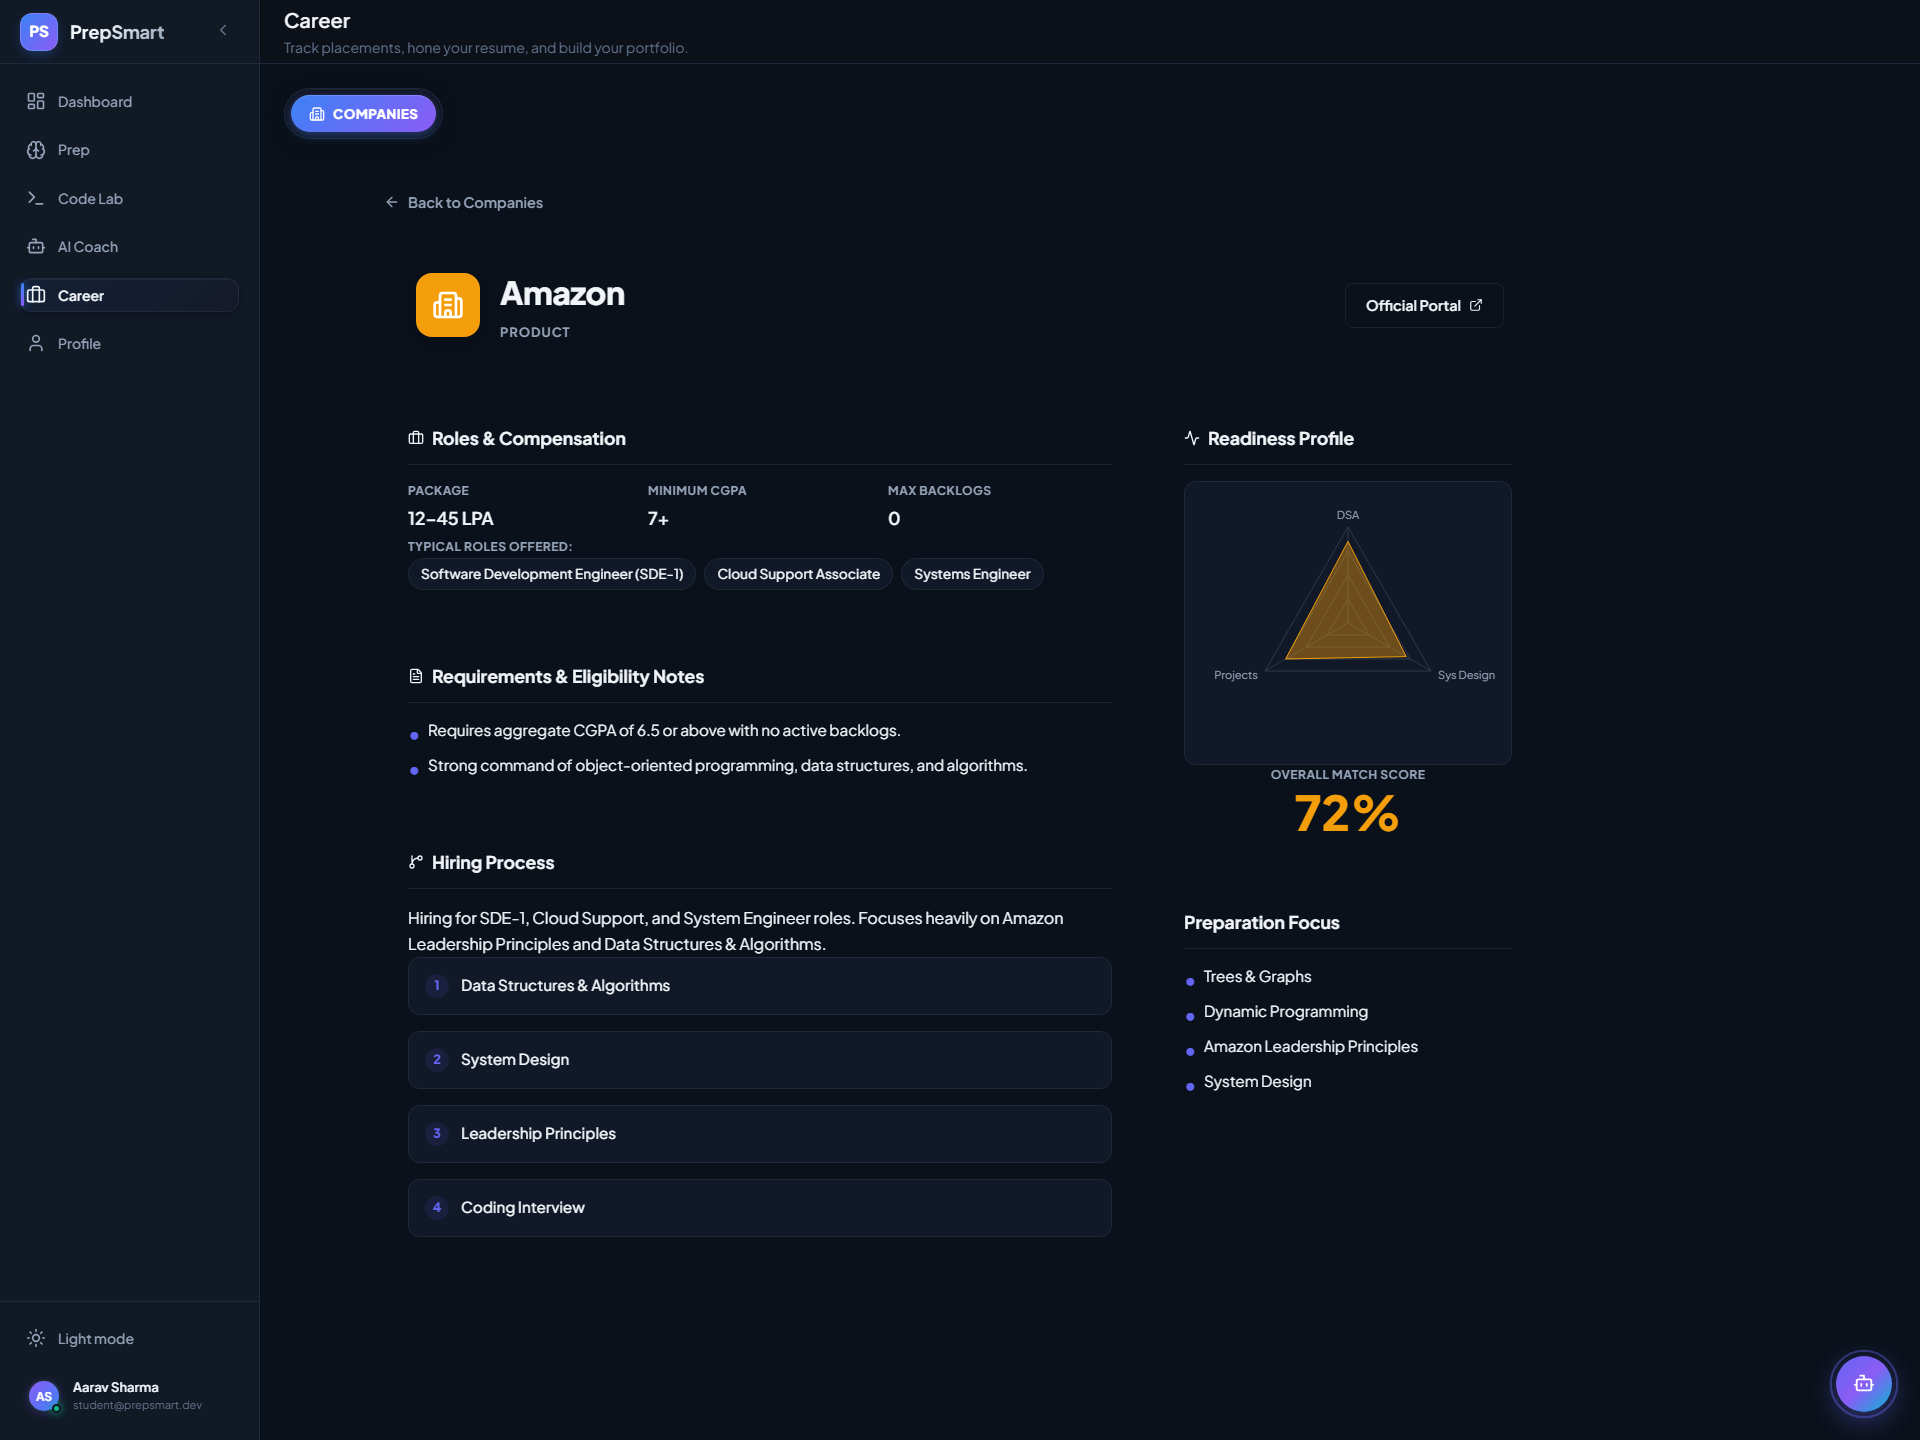
\includegraphics[width=0.95\textwidth]{Media/Chapter 5/company_detail.png}
\caption{Company Details Interface}
\label{fig:company_detail}
\end{figure}

Figure~\ref{fig:company_detail} illustrates the Company Details interface. This page presents company-specific preparation information including recommended topics, readiness indicators, coding expectations, interview requirements, and preparation progress.

The platform analyzes the student's completed learning activities and compares them with the selected company's expected preparation profile. Based on this analysis, readiness information and recommendations are displayed to guide further preparation.

\subsubsection*{Major Features}

\begin{itemize}

\item Company readiness score.

\item Preparation recommendations.

\item Topic requirements.

\item Coding readiness.

\item Interview readiness.

\item Progress visualization.

\end{itemize}

\section{Profile Management}

The Profile Management Module enables students to maintain their personal, academic, and professional information within the PrepSmart platform. It acts as the central repository for user-specific data that is utilized by various modules, including placement readiness analysis, portfolio generation, skills passport, and personalized learning recommendations.

The module provides dedicated interfaces for editing profile information and viewing the automatically generated Skills Passport.

\subsection{Profile Editor}

The Profile Editor allows students to create and update their personal profile by managing academic details, technical skills, career objectives, and placement preferences.

\begin{figure}[H]
\centering
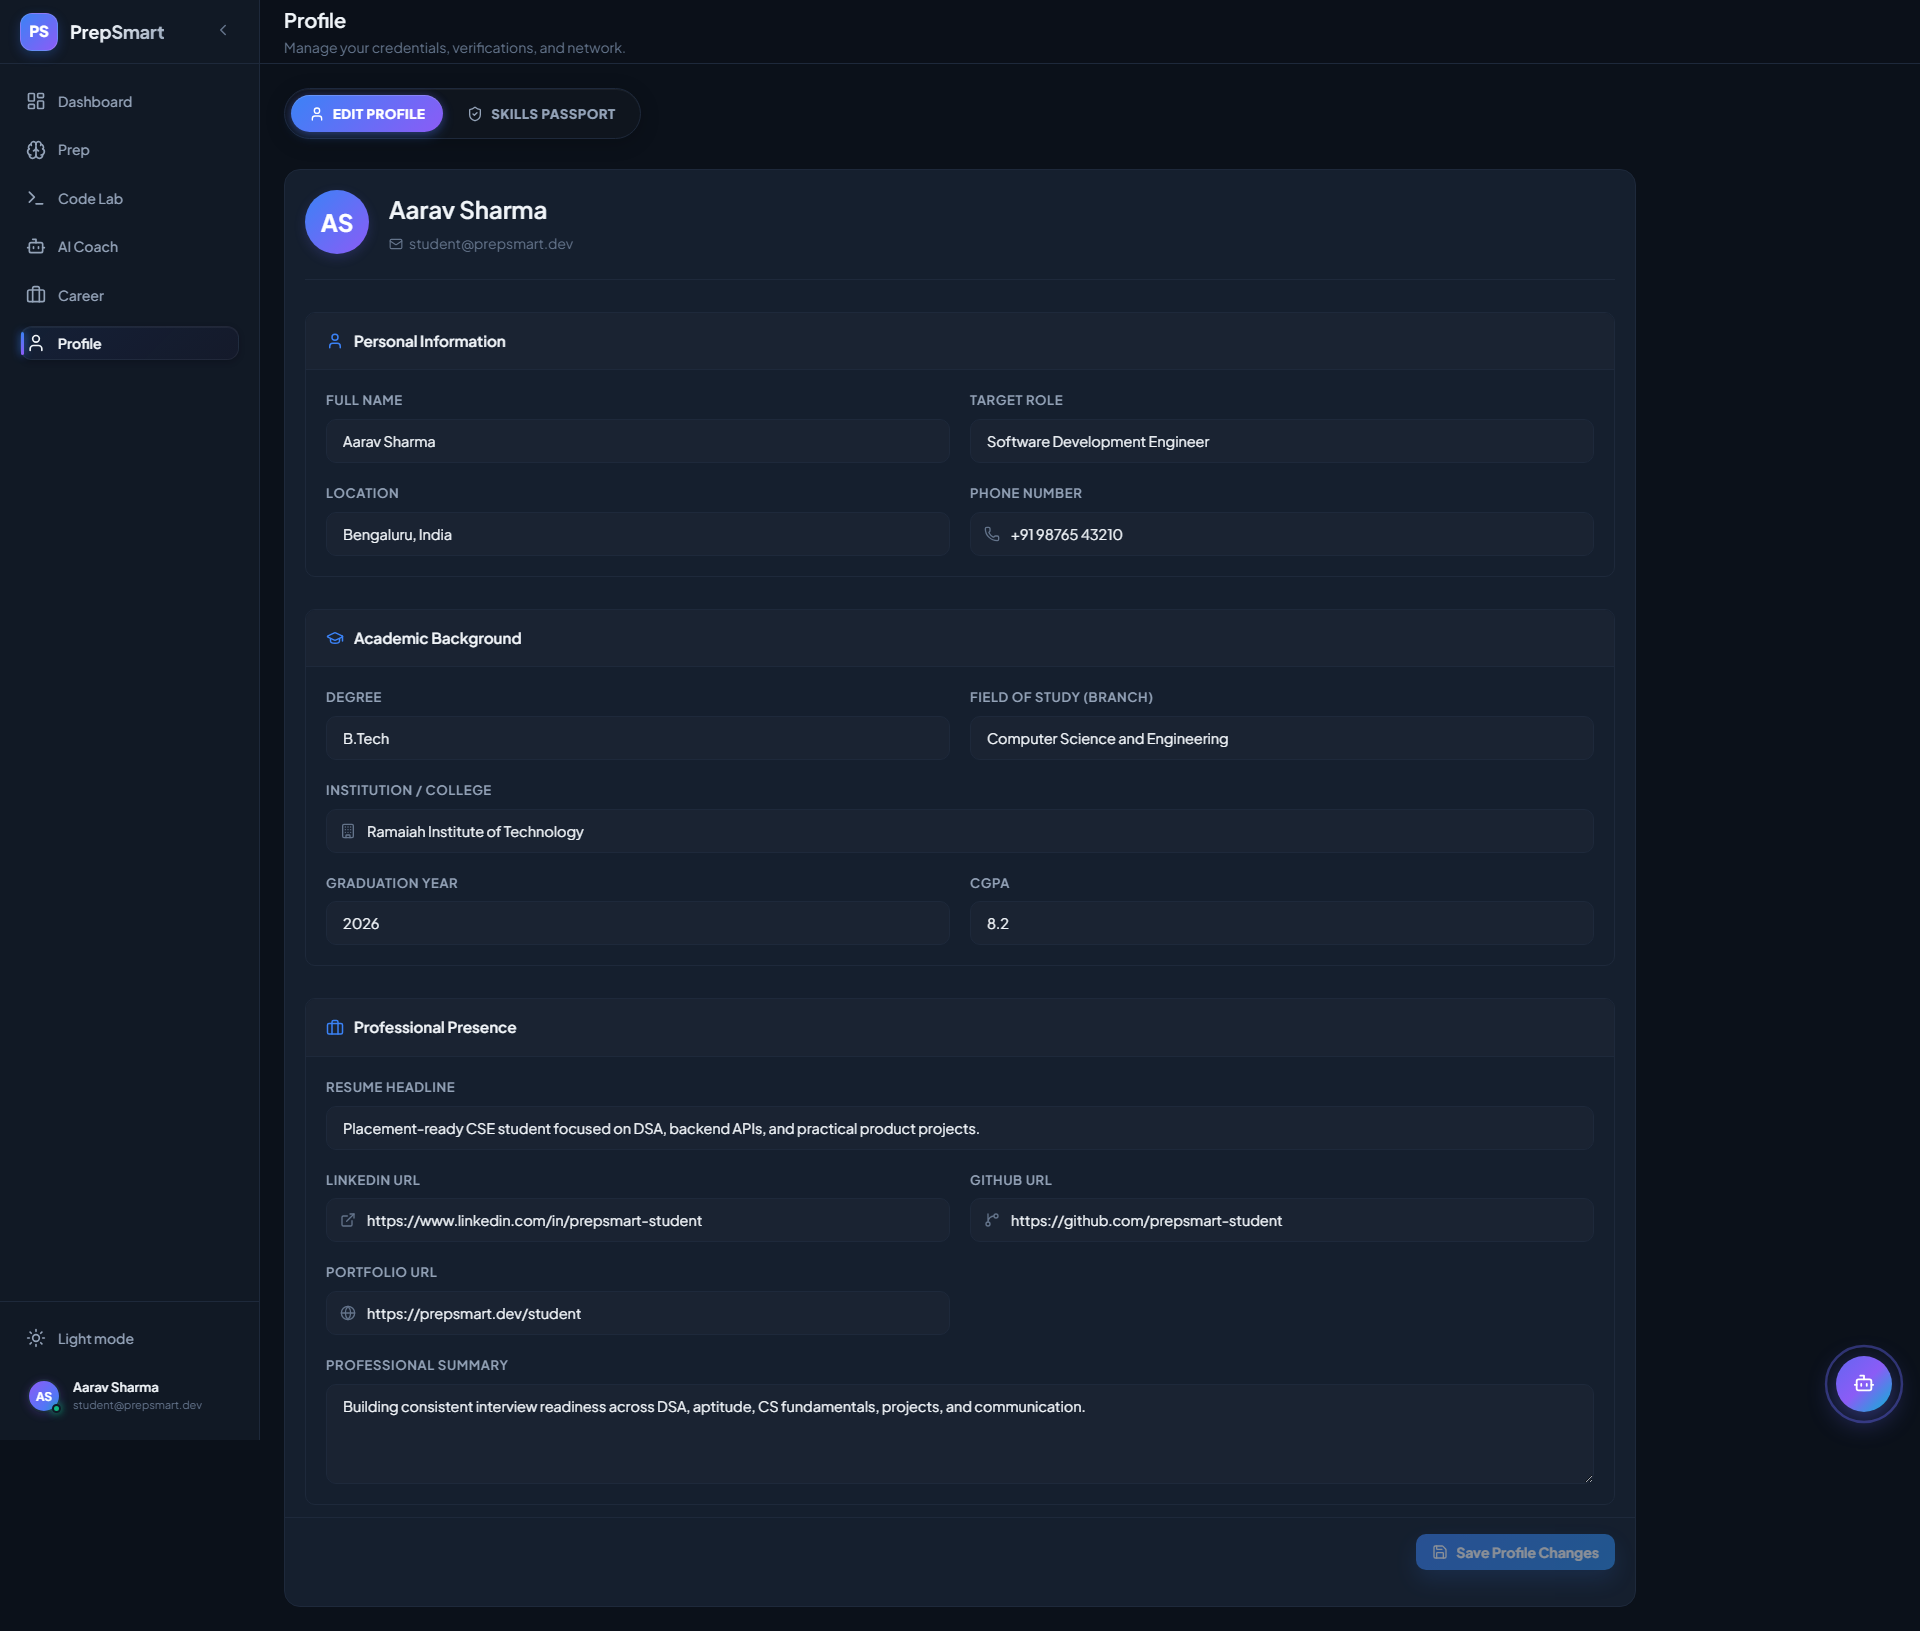
\includegraphics[width=0.95\textwidth]{Media/Chapter 5/profile_editor.png}
\caption{Profile Editor}
\label{fig:profile_editor}
\end{figure}

Figure~\ref{fig:profile_editor} illustrates the Profile Editor interface of PrepSmart. This page enables students to manage personal information, academic details, technical skills, target companies, career goals, and other profile-related information.

Users can update their profile whenever required, ensuring that the platform always maintains accurate information. The stored profile data is utilized by several modules, including dashboard analytics, company readiness evaluation, portfolio generation, and personalized placement recommendations.

The interface follows a simple and responsive design, allowing users to efficiently manage their information through organized input forms.

\subsubsection*{Major Features}

\begin{itemize}

\item Personal information management.

\item Academic profile management.

\item Technical skills management.

\item Target company preferences.

\item Career goal management.

\item Integration with placement analytics.

\end{itemize}

\subsection{Skills Passport}

The Skills Passport provides students with a consolidated view of their technical competencies, placement readiness, and overall employability. It summarizes learning progress and performance collected from different modules of the platform.

\begin{figure}[H]
\centering
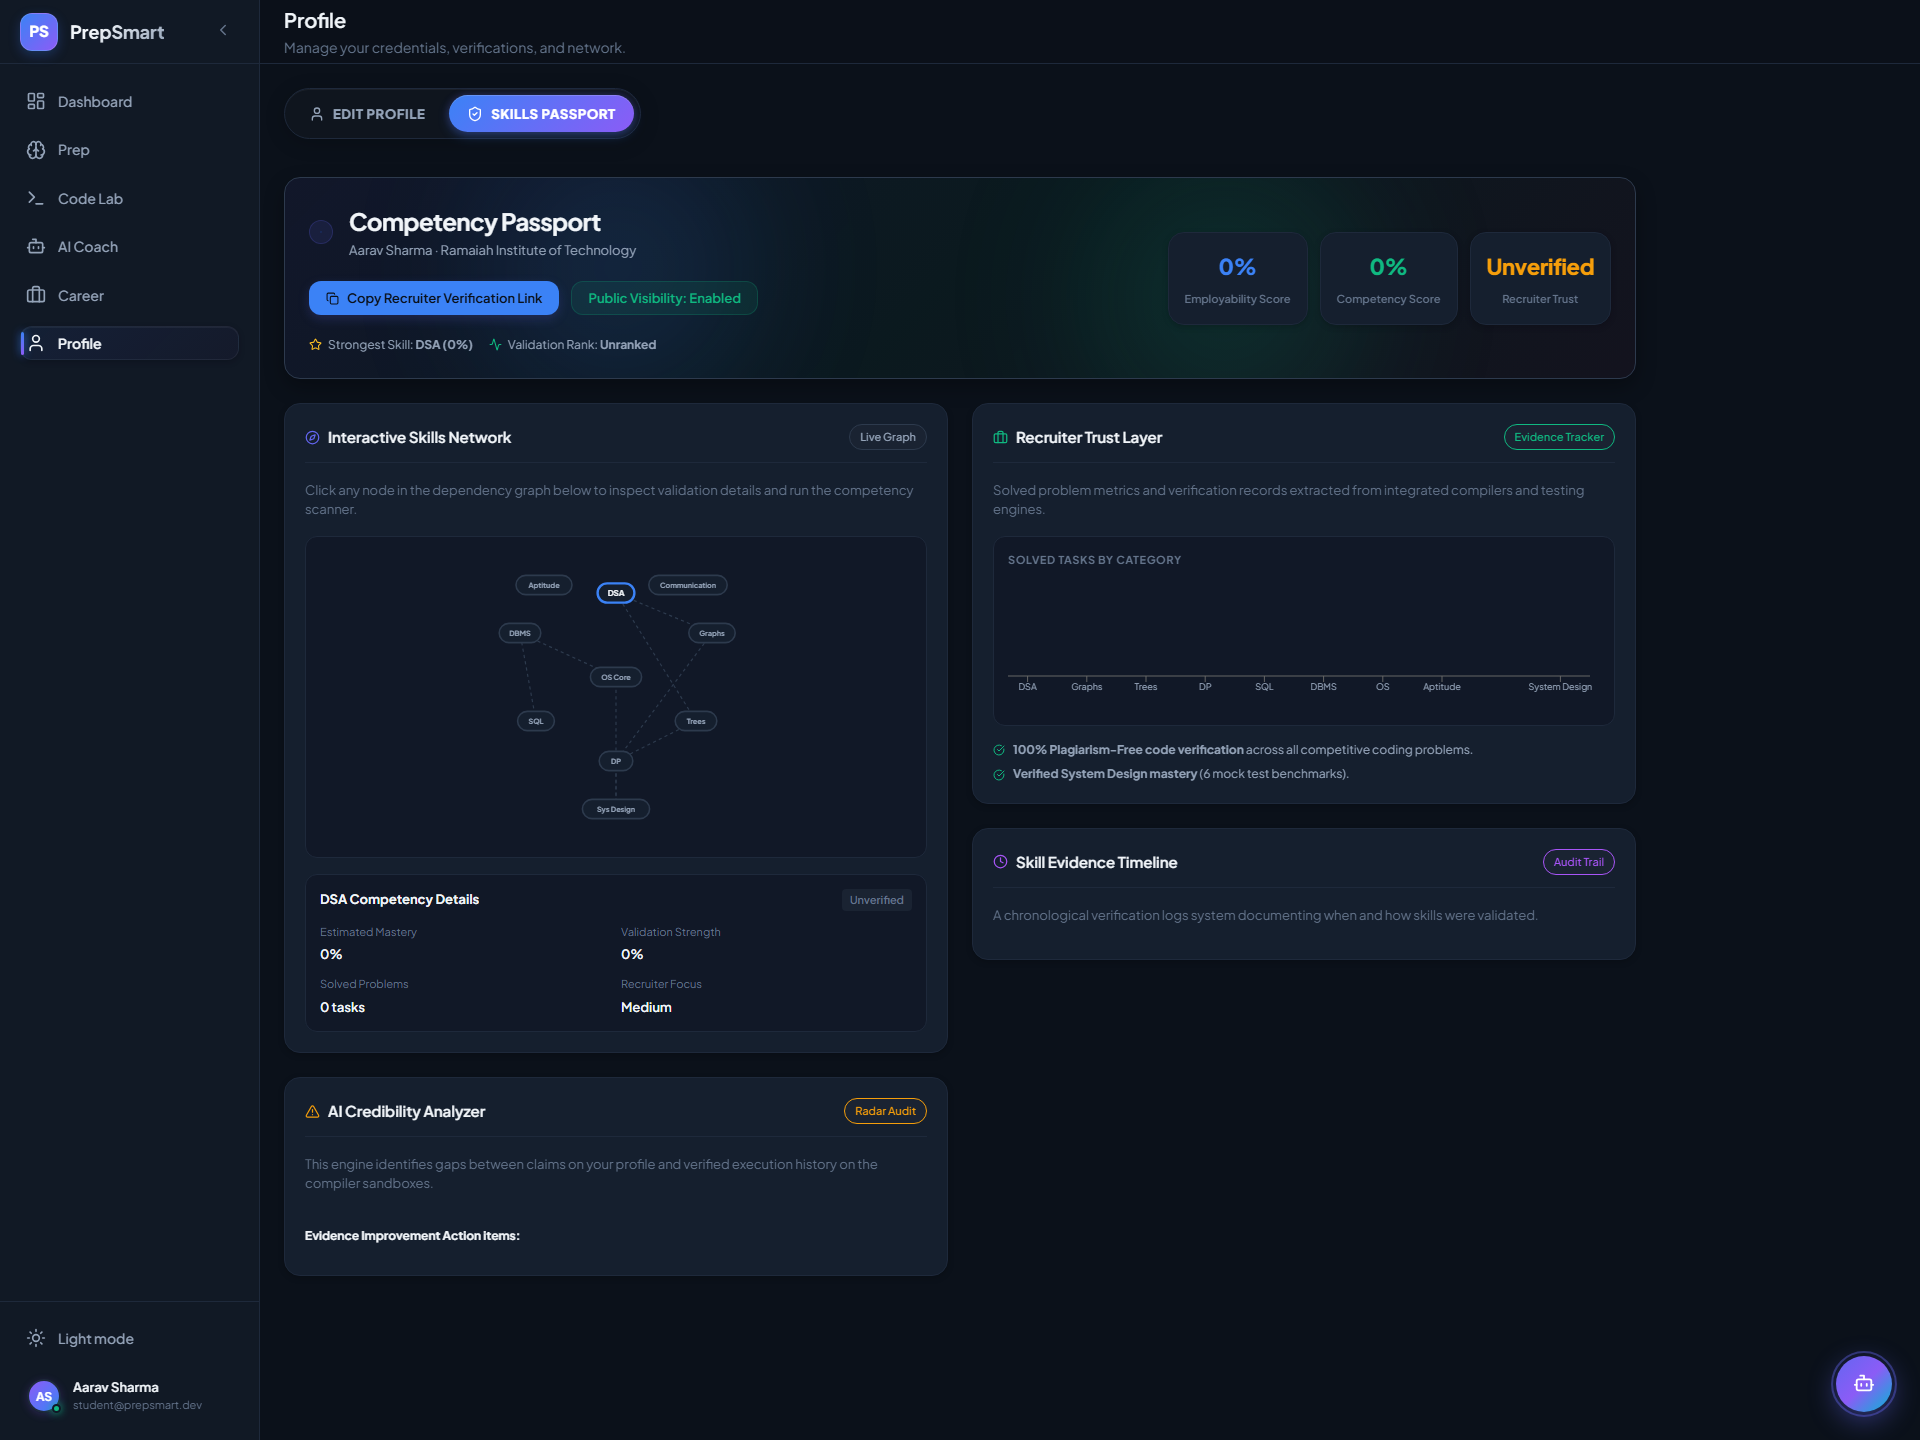
\includegraphics[width=0.95\textwidth]{Media/Chapter 5/skills_passport.png}
\caption{Skills Passport}
\label{fig:skills_passport}
\end{figure}

Figure~\ref{fig:skills_passport} presents the Skills Passport generated by PrepSmart. The interface summarizes the student's placement preparation using various performance indicators such as technical competency, coding activity, interview readiness, completed learning tracks, and overall employability.

The Skills Passport is generated automatically from the student's learning history and requires minimal manual intervention. It provides students with a comprehensive overview of their current preparation status while helping recruiters and placement coordinators understand the student's technical capabilities.

The information displayed within the Skills Passport is continuously updated whenever the student completes additional learning activities or assessments.

\subsubsection*{Major Features}

\begin{itemize}

\item Automatic employability profile generation.

\item Technical competency visualization.

\item Placement readiness indicators.

\item Coding performance summary.

\item Interview readiness tracking.

\item Continuous automatic updates.

\end{itemize}

\section{Shared Profiles}

PrepSmart enables students to share their professional profiles with recruiters, placement coordinators, and other external users through secure public links. The Shared Profiles module allows selected information to be viewed without exposing confidential user data.

\subsection{Shared Passport}

The Shared Passport interface presents a publicly accessible version of the student's Skills Passport that can be shared with recruiters and placement coordinators.

\begin{figure}[H]
\centering
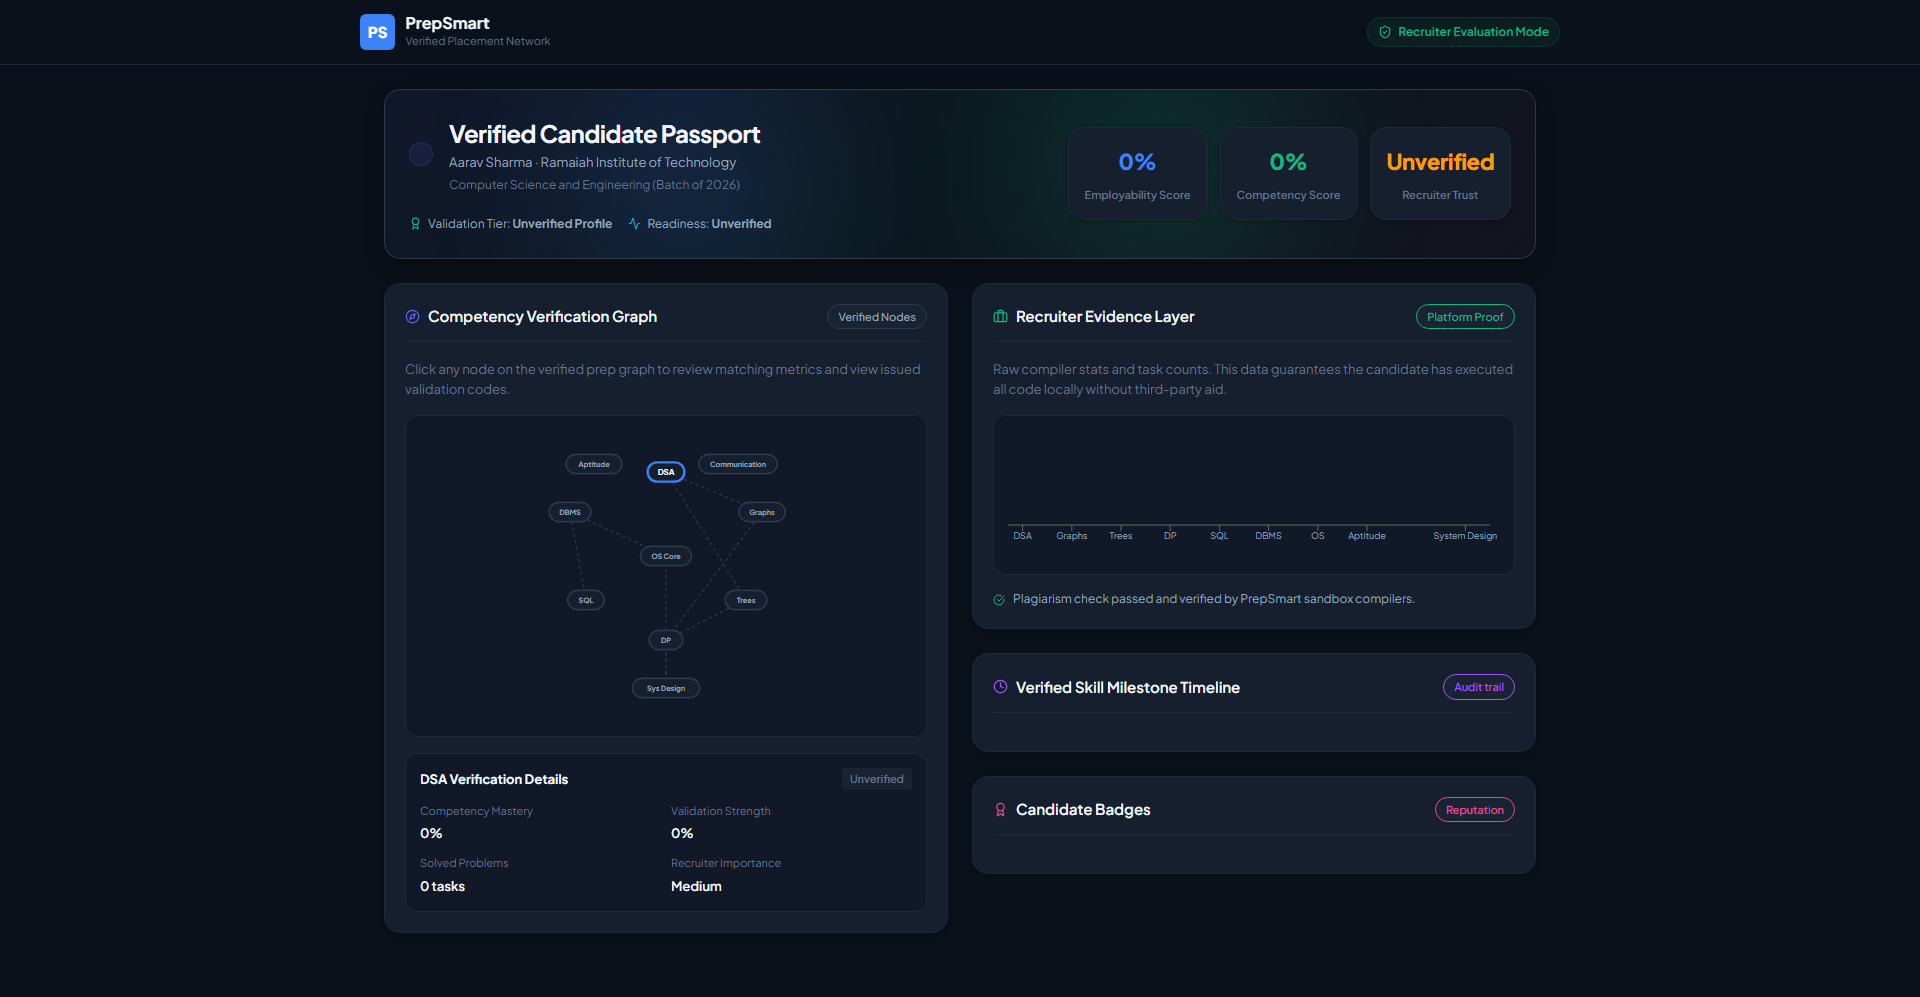
\includegraphics[width=0.95\textwidth]{Media/Chapter 5/shared_passport.png}
\caption{Shared Skills Passport}
\label{fig:shared_passport}
\end{figure}

Figure~\ref{fig:shared_passport} illustrates the publicly shared Skills Passport. This page presents selected placement readiness information while protecting confidential account details.

Recruiters can review technical competencies, learning progress, interview readiness, and employability indicators without requiring direct access to the student's PrepSmart account.

\subsection{Shared Portfolio}

The Shared Portfolio enables students to publicly showcase their projects, technical skills, certifications, and professional achievements using a dedicated shareable webpage.

\begin{figure}[H]
\centering
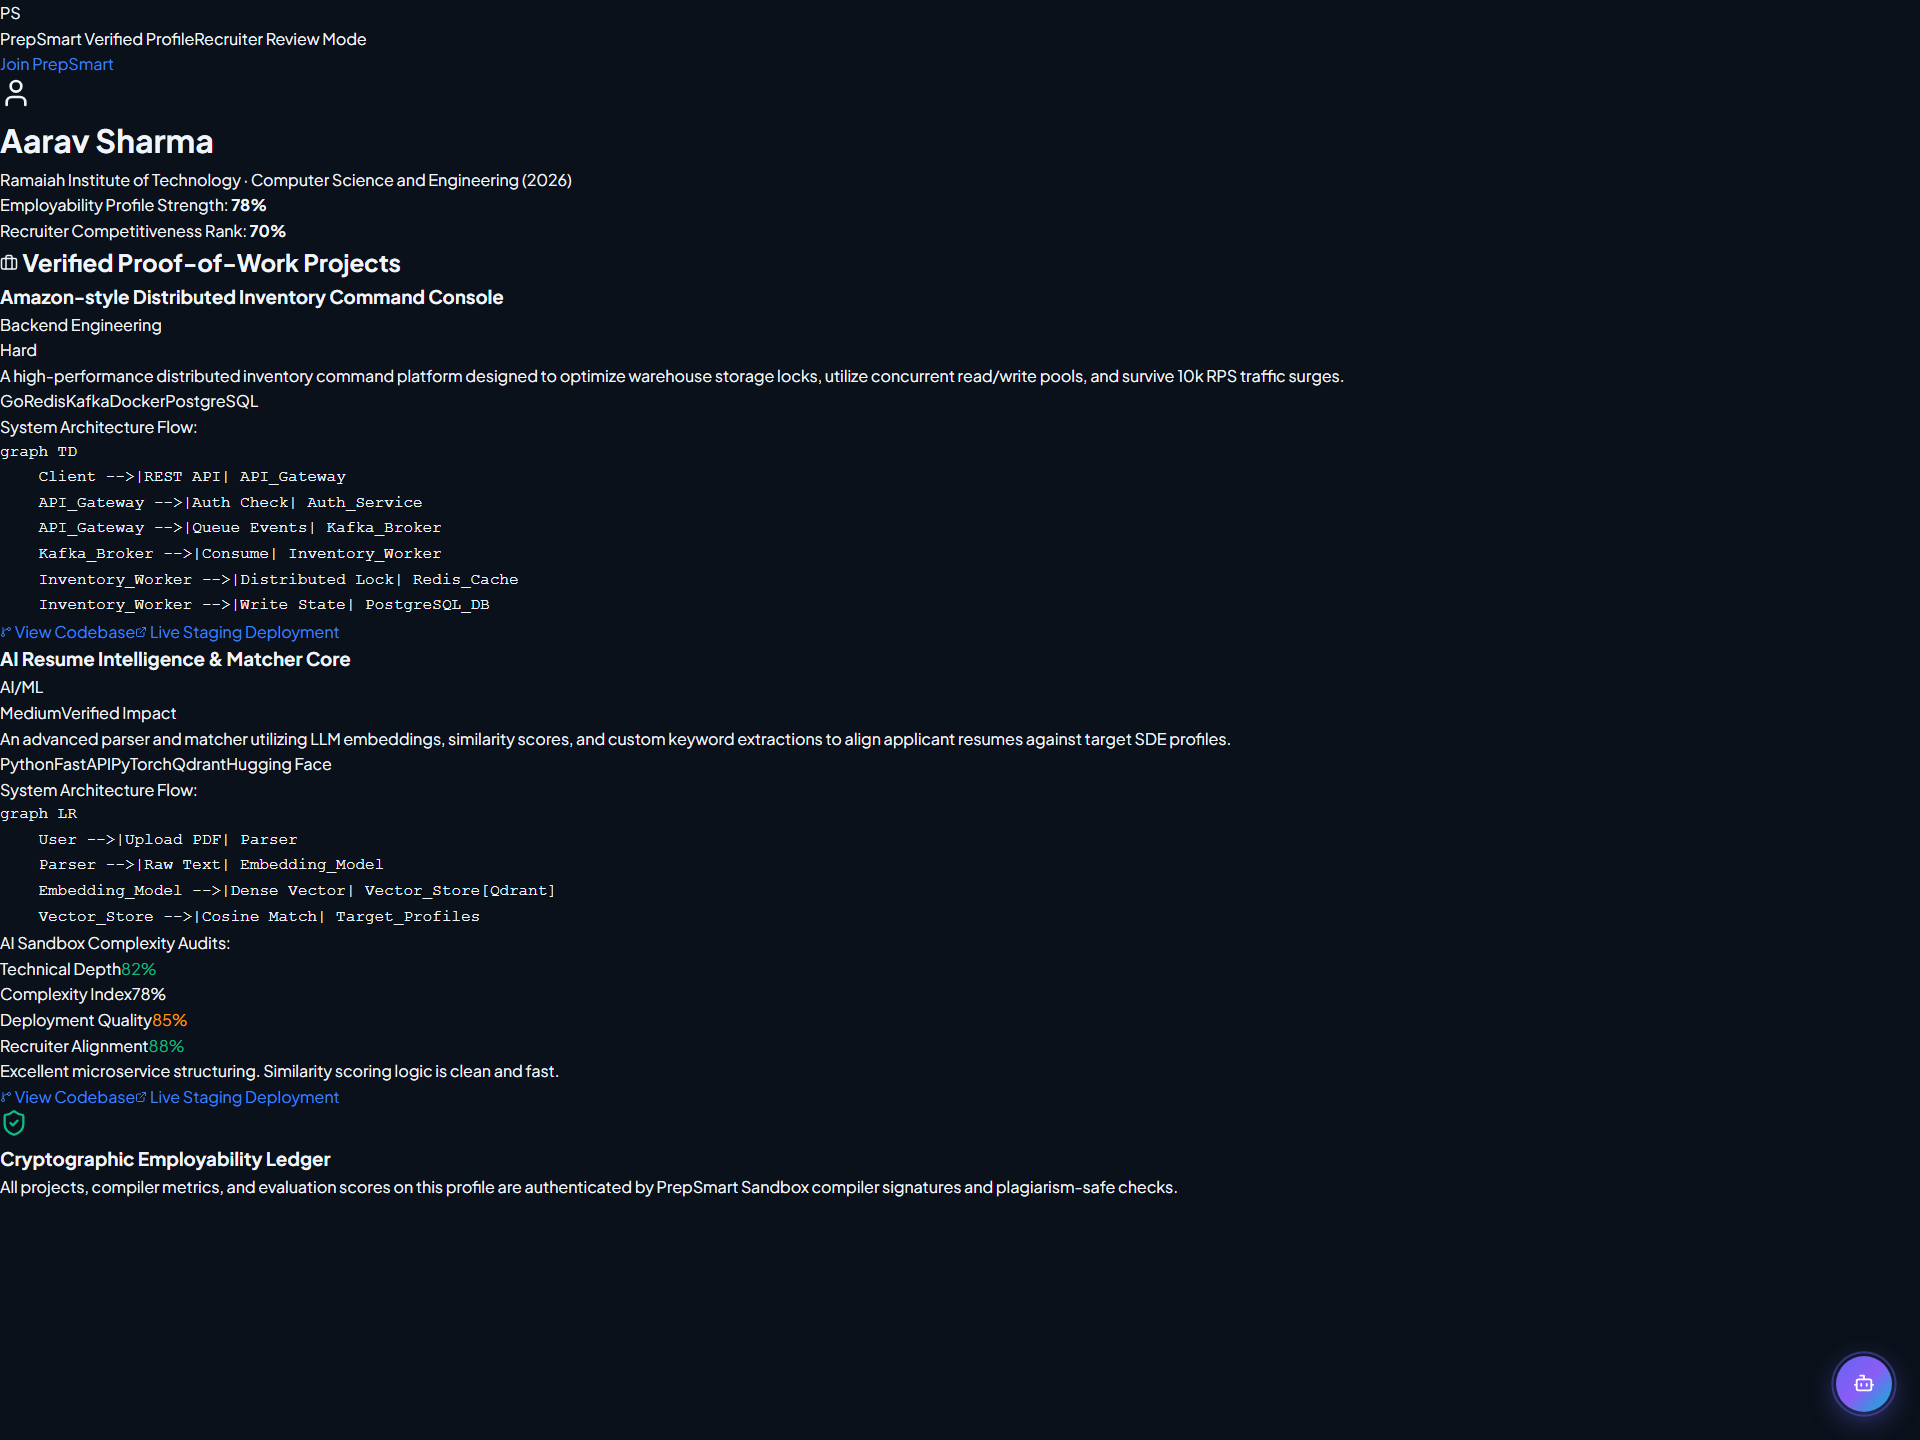
\includegraphics[width=0.95\textwidth]{Media/Chapter 5/shared_portfolio.png}
\caption{Shared Portfolio}
\label{fig:shared_portfolio}
\end{figure}

Figure~\ref{fig:shared_portfolio} presents the publicly accessible portfolio generated by PrepSmart. The page organizes the student's projects, skills, certifications, academic profile, and other professional achievements into a structured format suitable for recruiters.

The portfolio is generated dynamically from information already stored within the platform, eliminating the need for students to manually create separate portfolio websites.

\subsection*{Major Features of Shared Profiles}

\begin{itemize}

\item Public profile sharing.

\item Secure access through unique links.

\item Recruiter-friendly presentation.

\item Dynamic profile generation.

\item Automatic synchronization with user data.

\item Privacy protection for confidential information.

\end{itemize}

\section{Analytics Dashboard}

The Analytics Dashboard provides students with a detailed analysis of their placement preparation by presenting various performance indicators and statistical visualizations. Unlike the main dashboard, which provides an overall summary, the analytics module focuses on detailed performance evaluation, enabling students to identify strengths, weaknesses, and improvement opportunities.

The interface continuously updates analytical information using data collected from learning activities, coding practice, mock tests, interview sessions, and company preparation modules.

\begin{figure}[H]
\centering
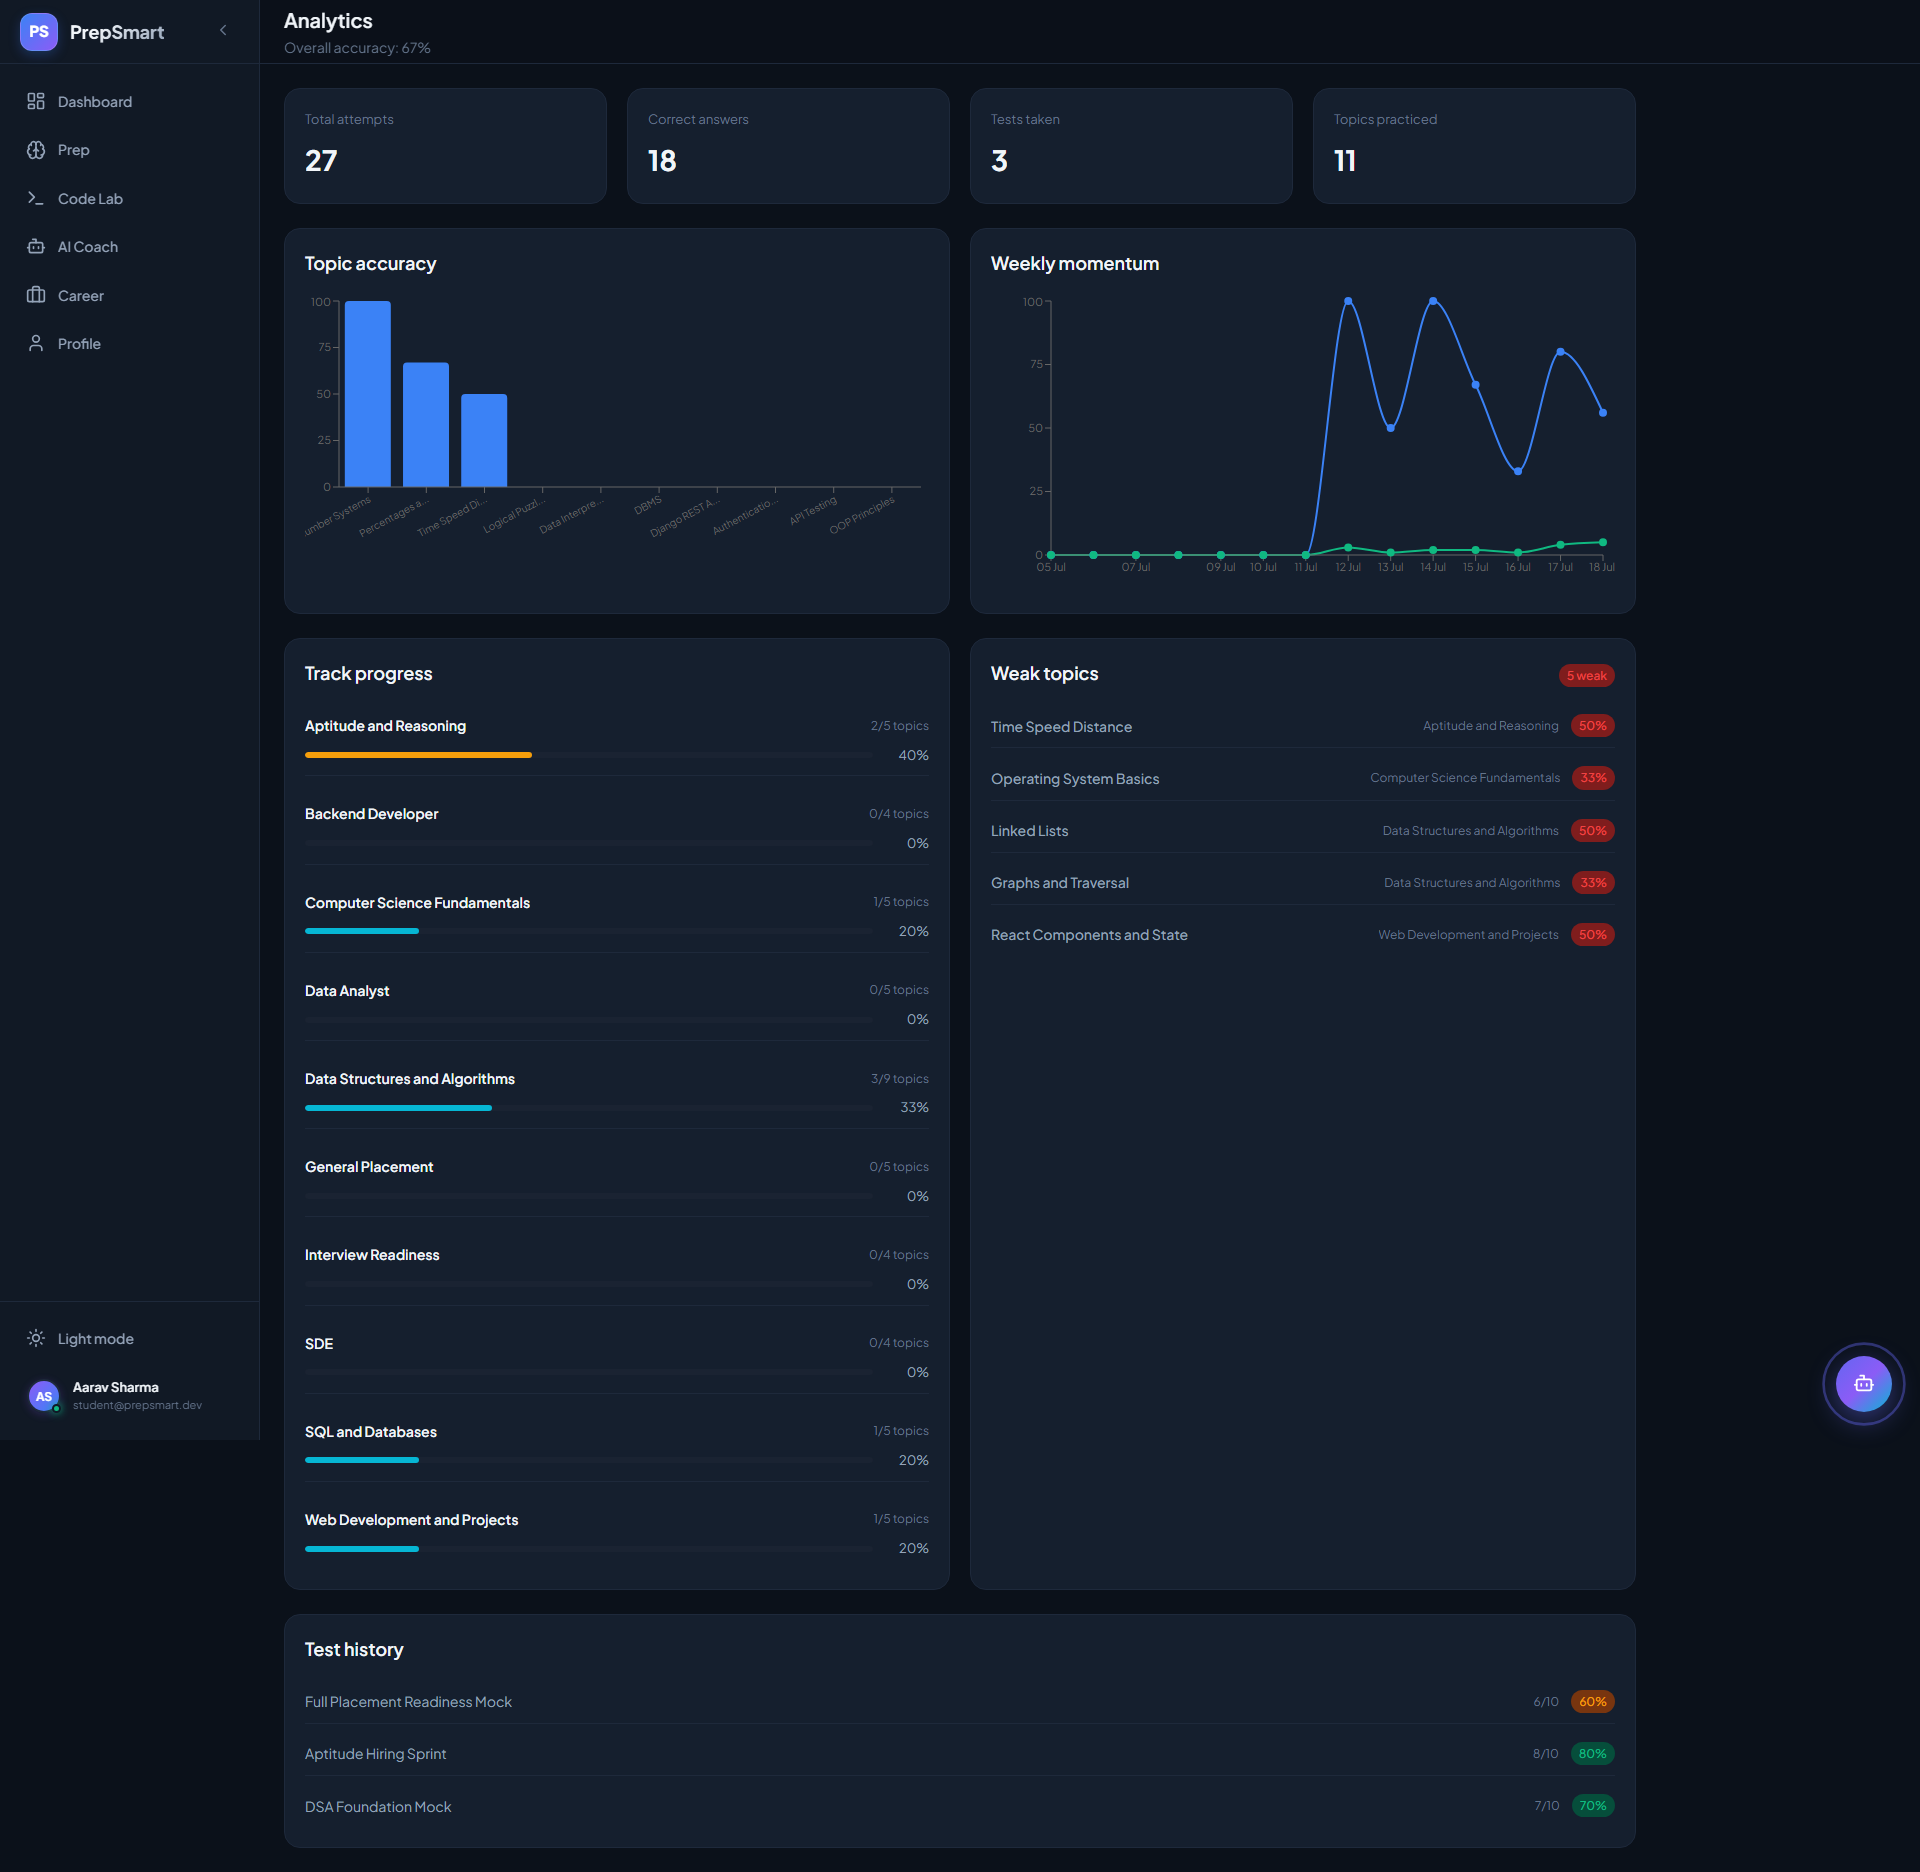
\includegraphics[width=0.95\textwidth]{Media/Chapter 5/analytics.png}
\caption{Analytics Dashboard}
\label{fig:analytics_dashboard}
\end{figure}

Figure~\ref{fig:analytics_dashboard} illustrates the Analytics Dashboard of PrepSmart. The page presents various statistical summaries and graphical representations that help students evaluate their overall preparation progress.

The dashboard displays information such as topic completion percentages, coding activity, quiz accuracy, interview performance, company readiness, and learning trends. Interactive charts and progress indicators simplify the interpretation of performance data and enable students to identify areas requiring additional attention.

Since the displayed information is generated dynamically from the backend database, students always receive up-to-date analytical insights based on their latest activities.

\subsection*{Major Features}

\begin{itemize}

\item Learning progress analytics.

\item Coding performance statistics.

\item Interview performance analysis.

\item Company readiness visualization.

\item Interactive charts.

\item Real-time analytical updates.

\end{itemize}

\section{Settings}

The Settings module enables users to personalize their experience within the PrepSmart platform. It provides configuration options related to user preferences, application appearance, notification settings, and account management.

\begin{figure}[H]
\centering
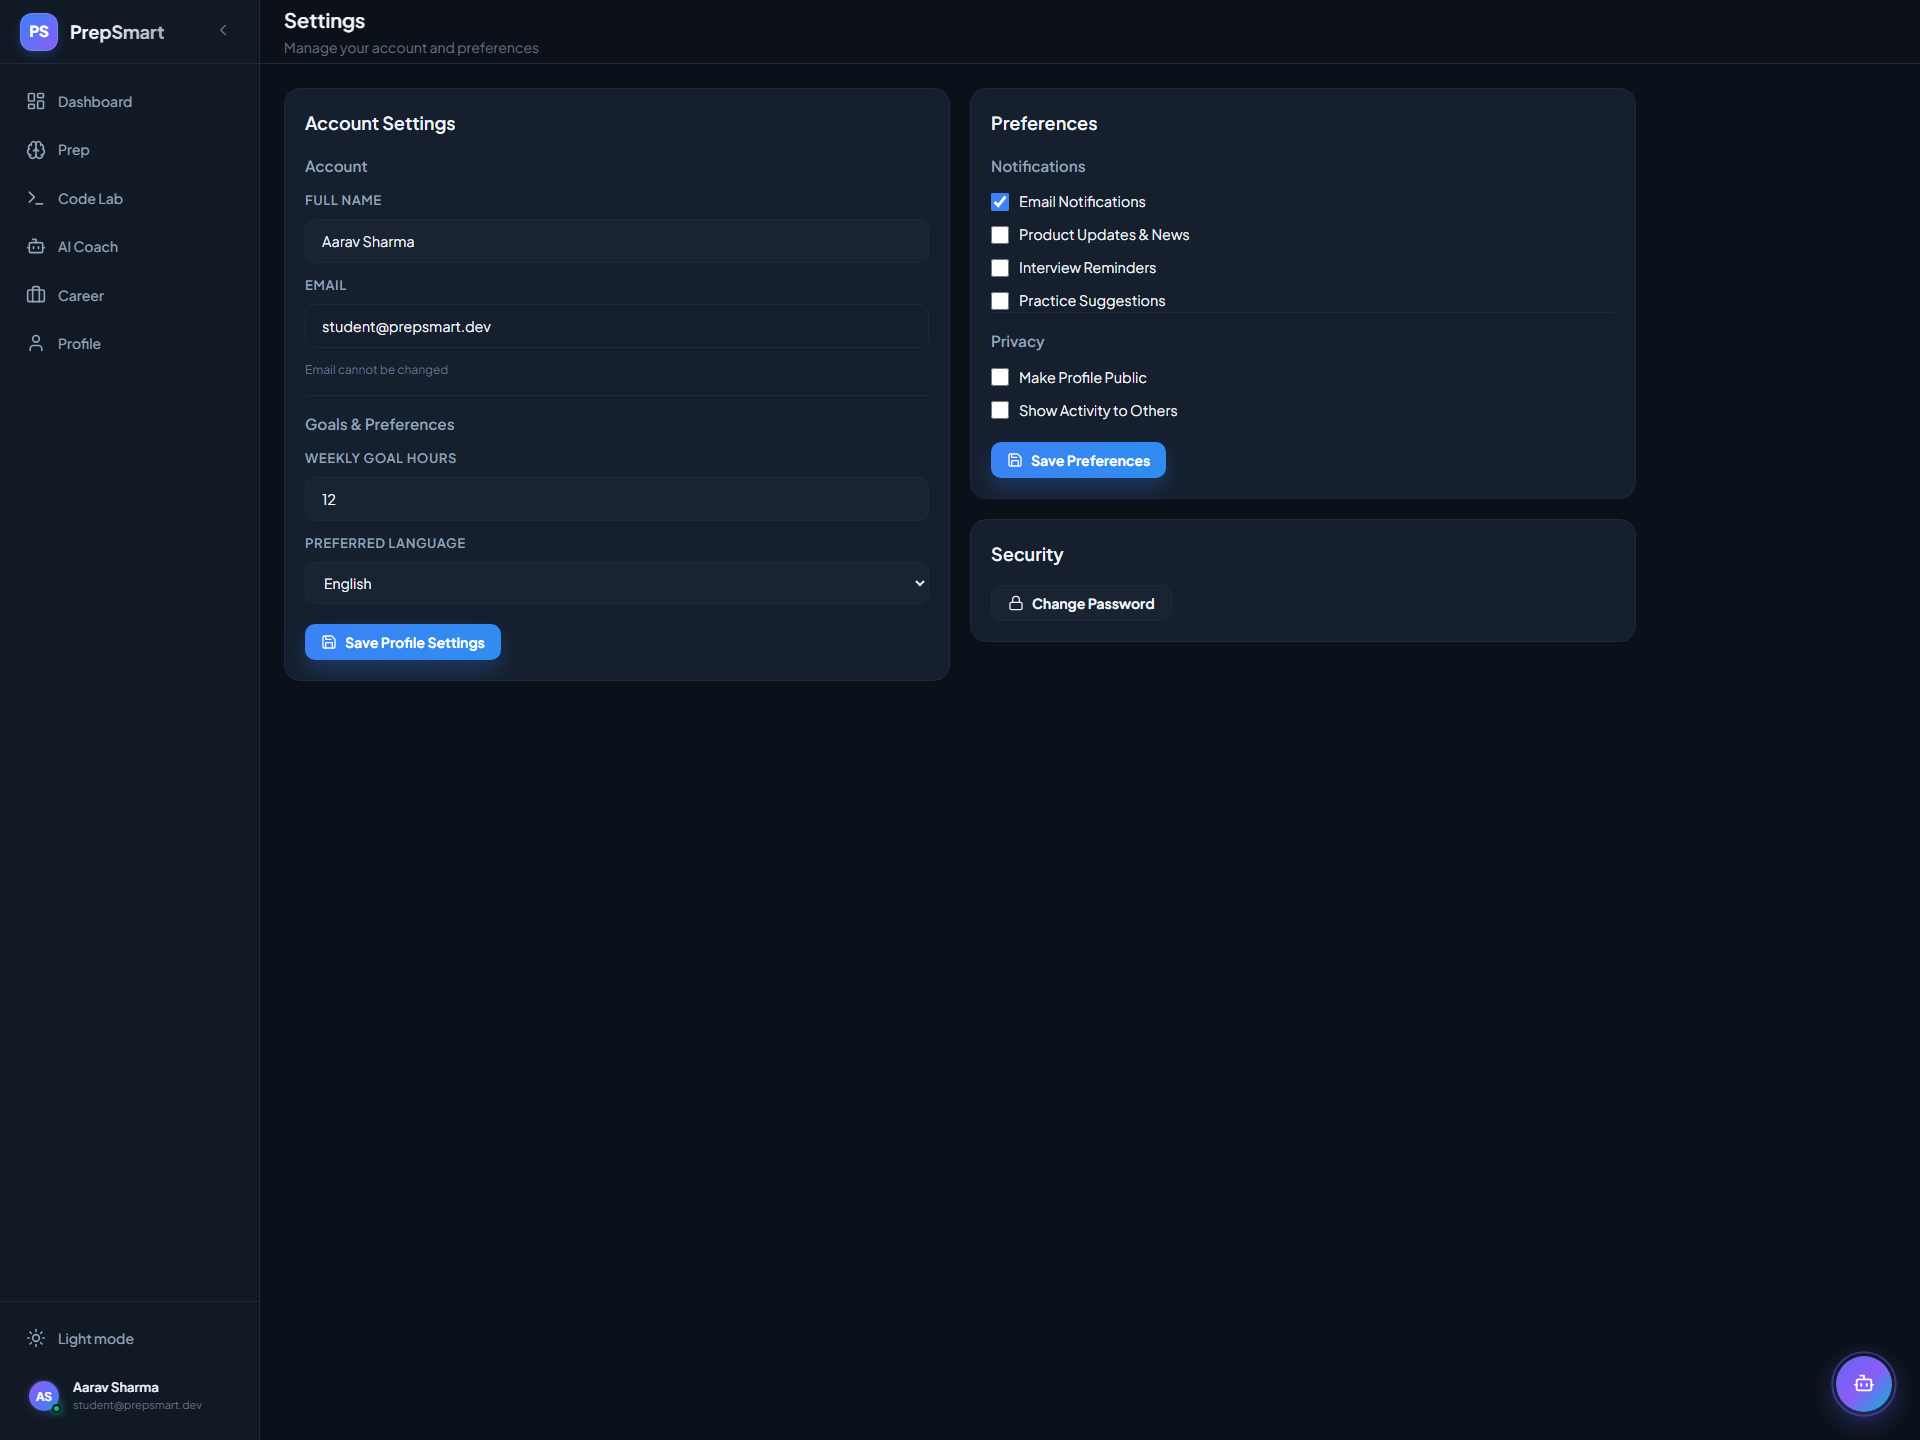
\includegraphics[width=0.95\textwidth]{Media/Chapter 5/settings.png}
\caption{Settings Interface}
\label{fig:settings}
\end{figure}

Figure~\ref{fig:settings} presents the Settings interface of PrepSmart. Through this page, users can manage their application preferences and personalize the overall user experience.

The interface provides options for updating account settings, adjusting application preferences, managing notifications, and configuring other personalized options. The responsive layout ensures that settings can be modified conveniently across different devices.

\subsection*{Major Features}

\begin{itemize}

\item User preference management.

\item Account settings.

\item Notification configuration.

\item Personalized application experience.

\item Responsive interface.

\end{itemize}

\section{Administration Module}

The Administration Module enables authorized administrators to manage the entire PrepSmart platform. Through the Django administrative interface, administrators can create, update, delete, and monitor different entities within the system. This centralized management simplifies content administration and ensures the smooth operation of the platform.

\subsection{User Management}

\begin{figure}[H]
\centering
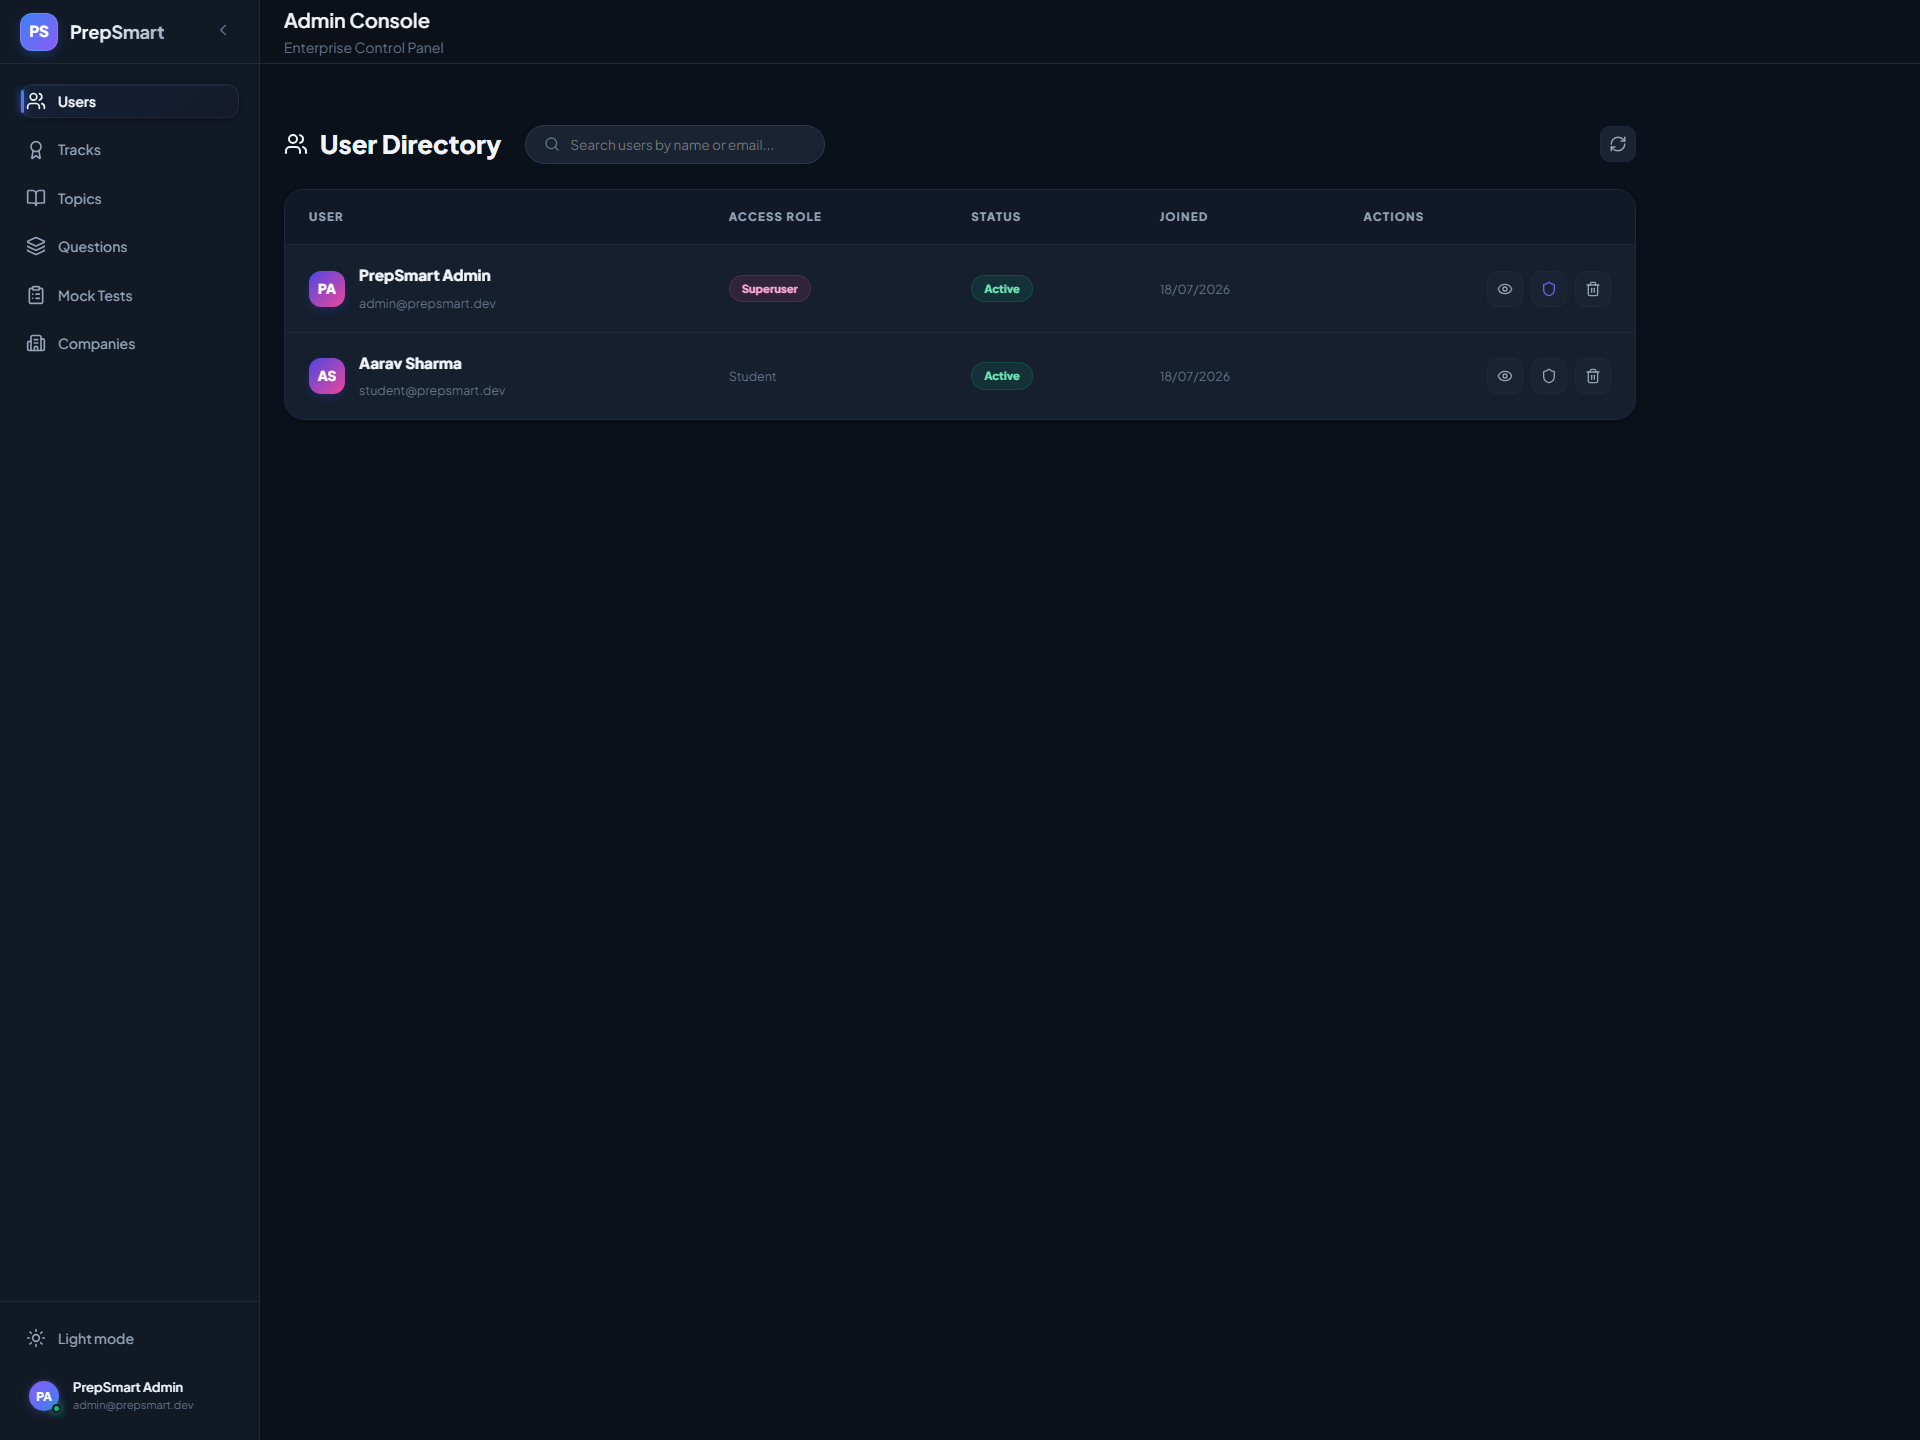
\includegraphics[width=0.90\textwidth]{Media/Chapter 5/admin_users.png}
\caption{Administration - User Management}
\label{fig:admin_users}
\end{figure}

The User Management interface enables administrators to monitor registered users, manage user accounts, update permissions, and perform administrative actions when required.

\subsection{Track Management}

\begin{figure}[H]
\centering
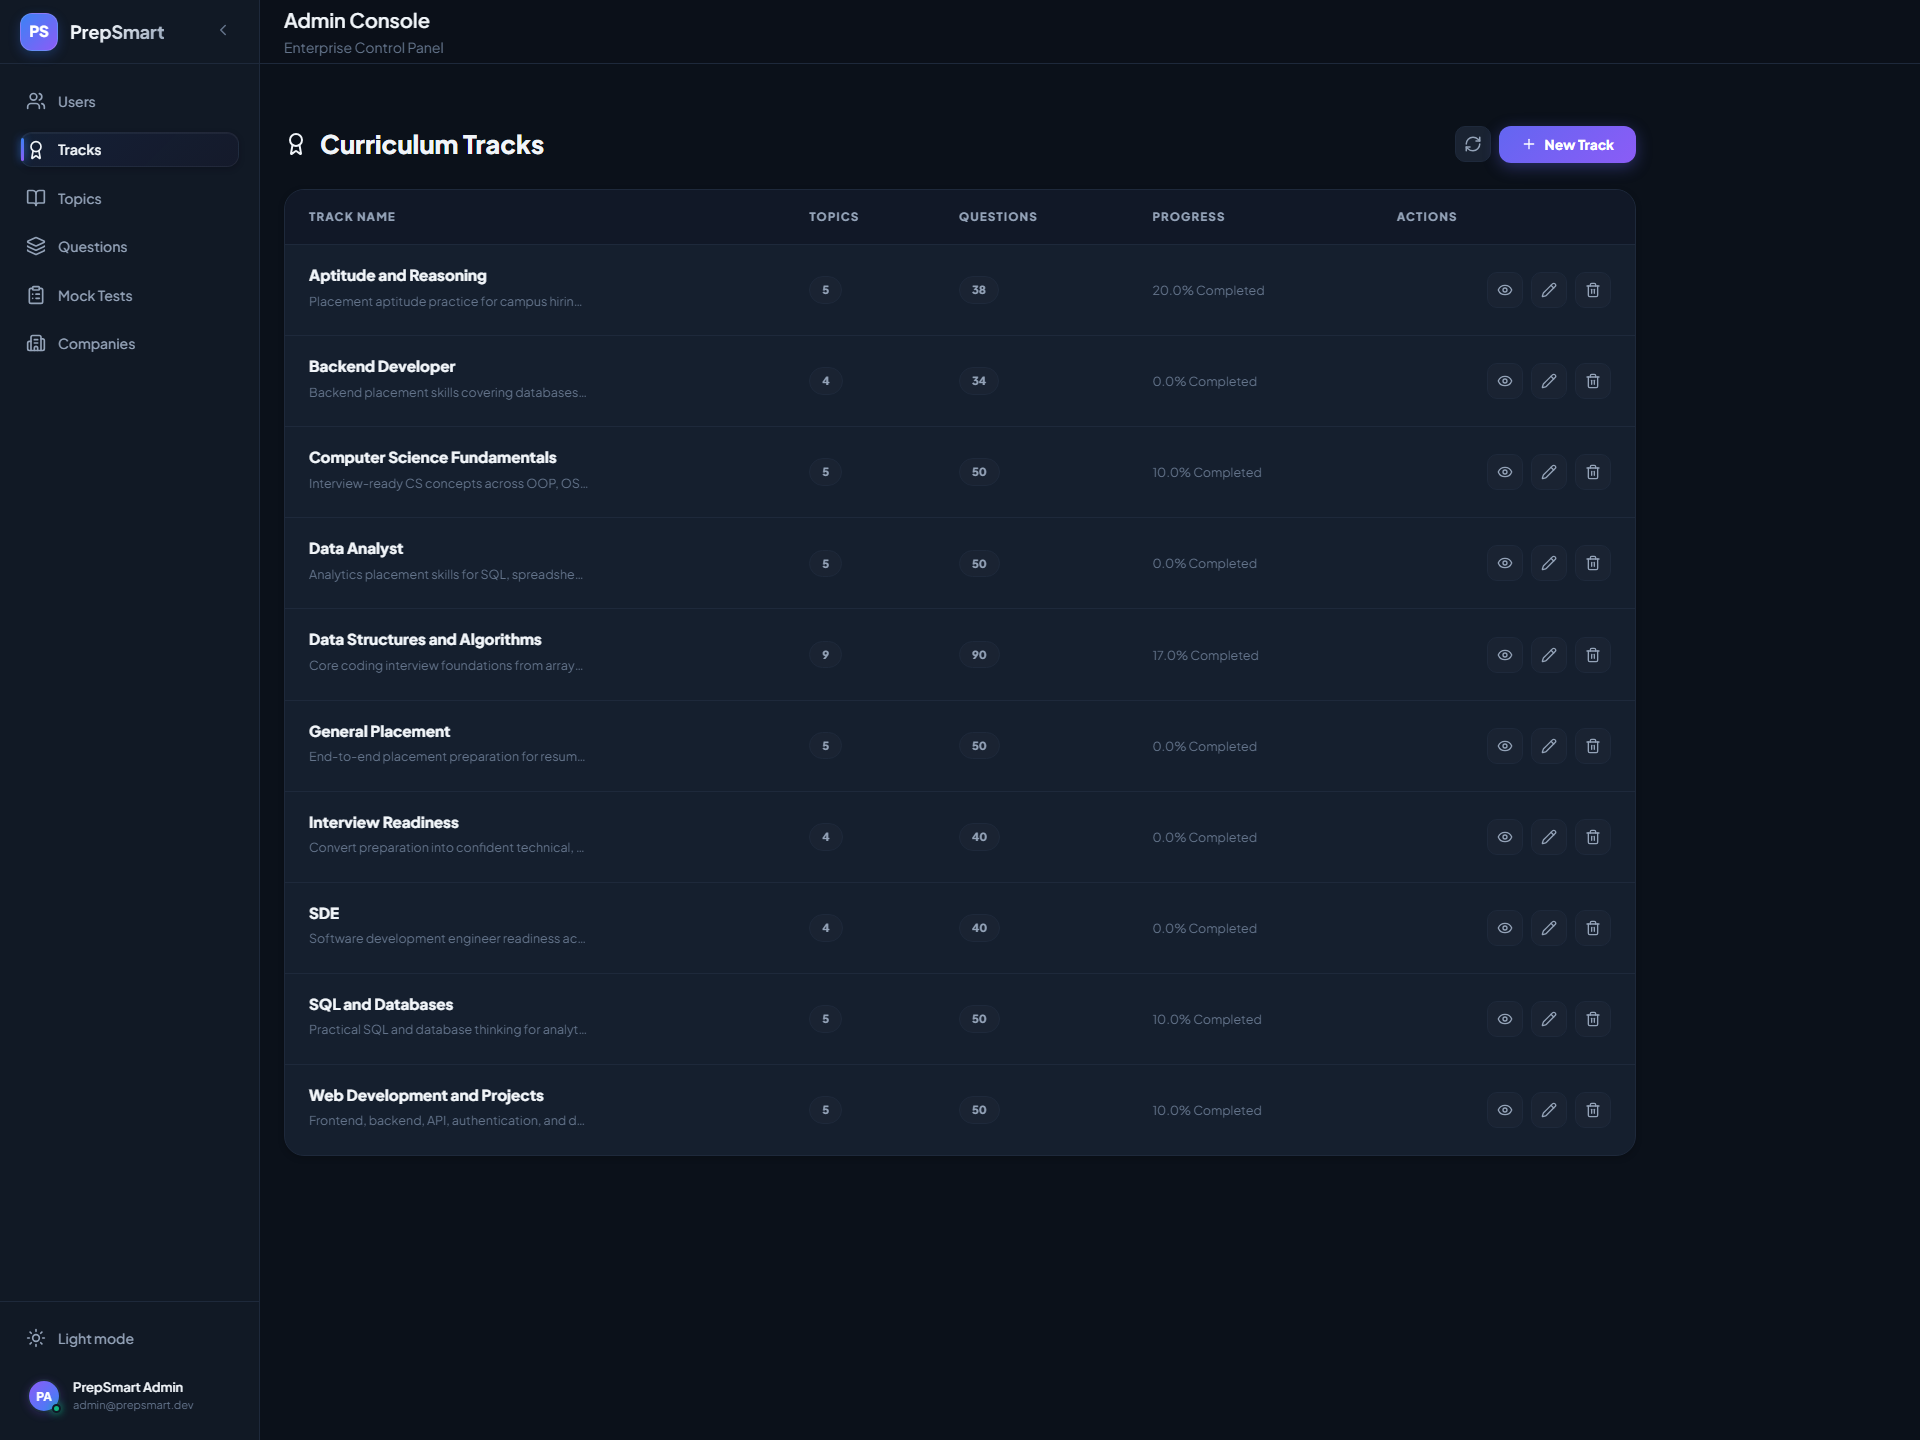
\includegraphics[width=0.90\textwidth]{Media/Chapter 5/admin_tracks.png}
\caption{Administration - Track Management}
\label{fig:admin_tracks}
\end{figure}

Administrators manage learning tracks through this interface by creating new preparation domains, updating existing tracks, and organizing educational content.

\subsection{Topic Management}

\begin{figure}[H]
\centering
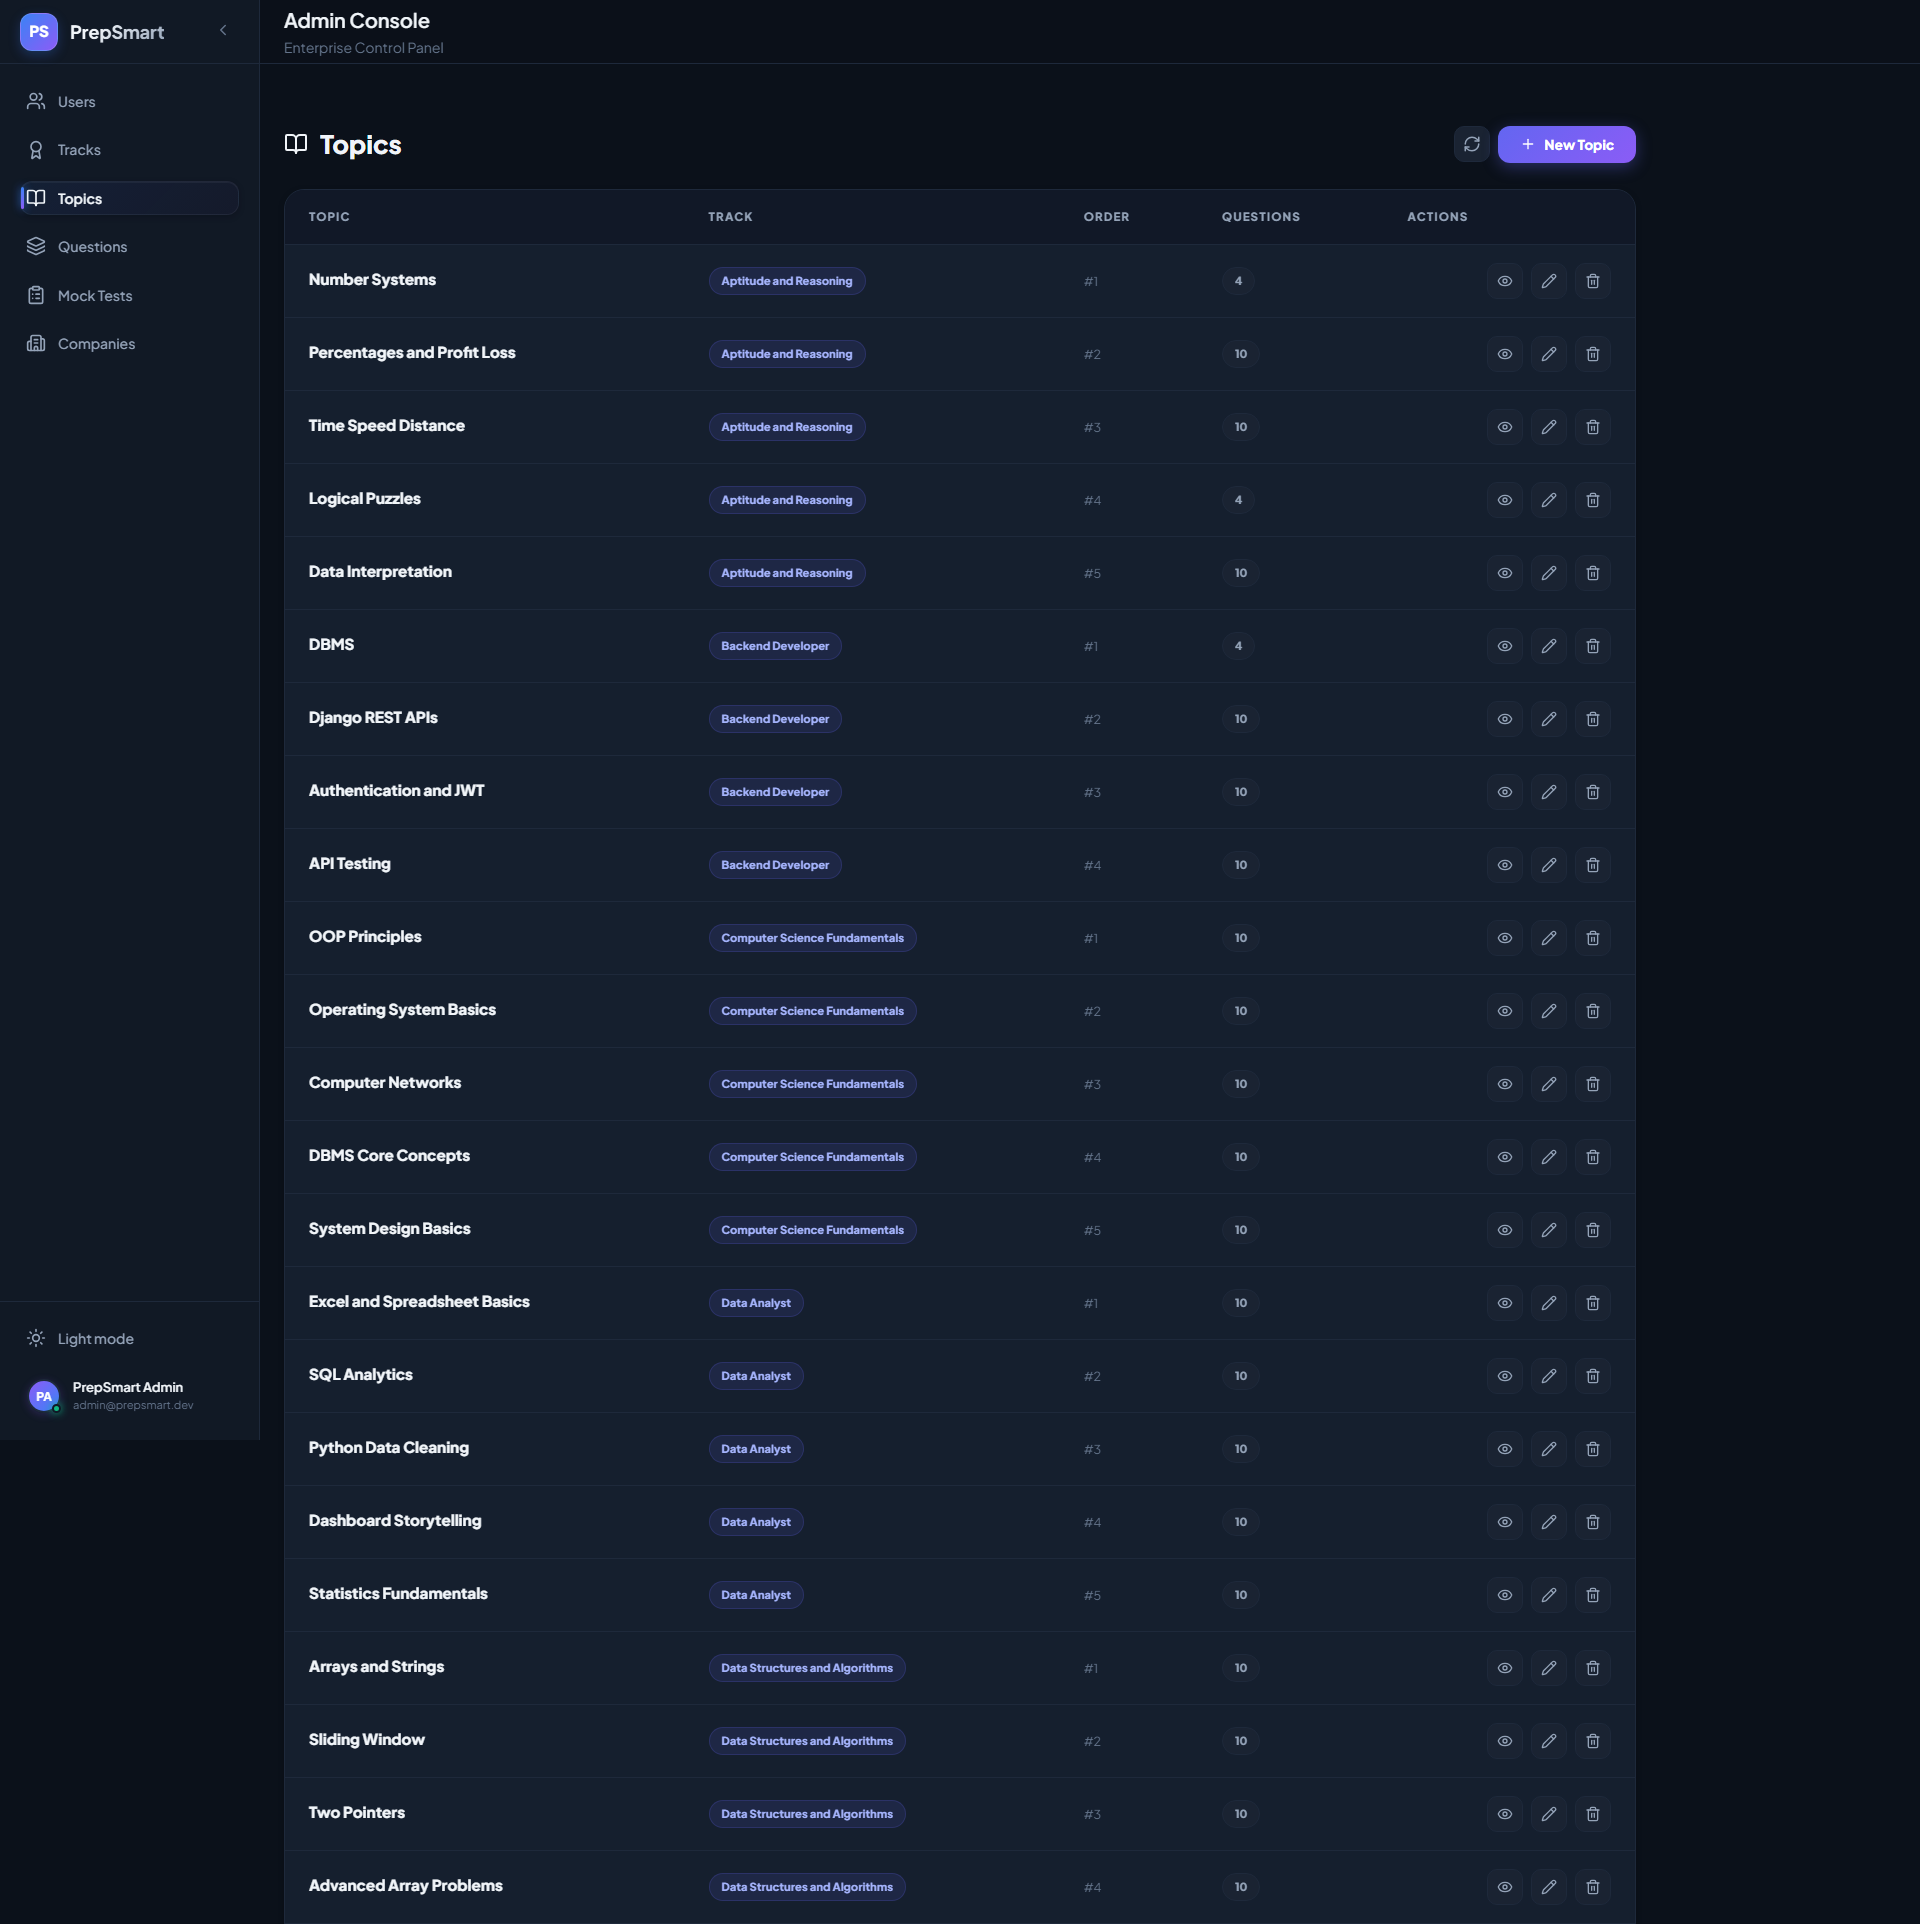
\includegraphics[width=0.90\textwidth]{Media/Chapter 5/admin_topics.png}
\caption{Administration - Topic Management}
\label{fig:admin_topics}
\end{figure}

The Topic Management interface enables administrators to organize individual learning topics, descriptions, prerequisites, and learning sequences used throughout the placement preparation module.

\subsection{Question Management}

\begin{figure}[H]
\centering
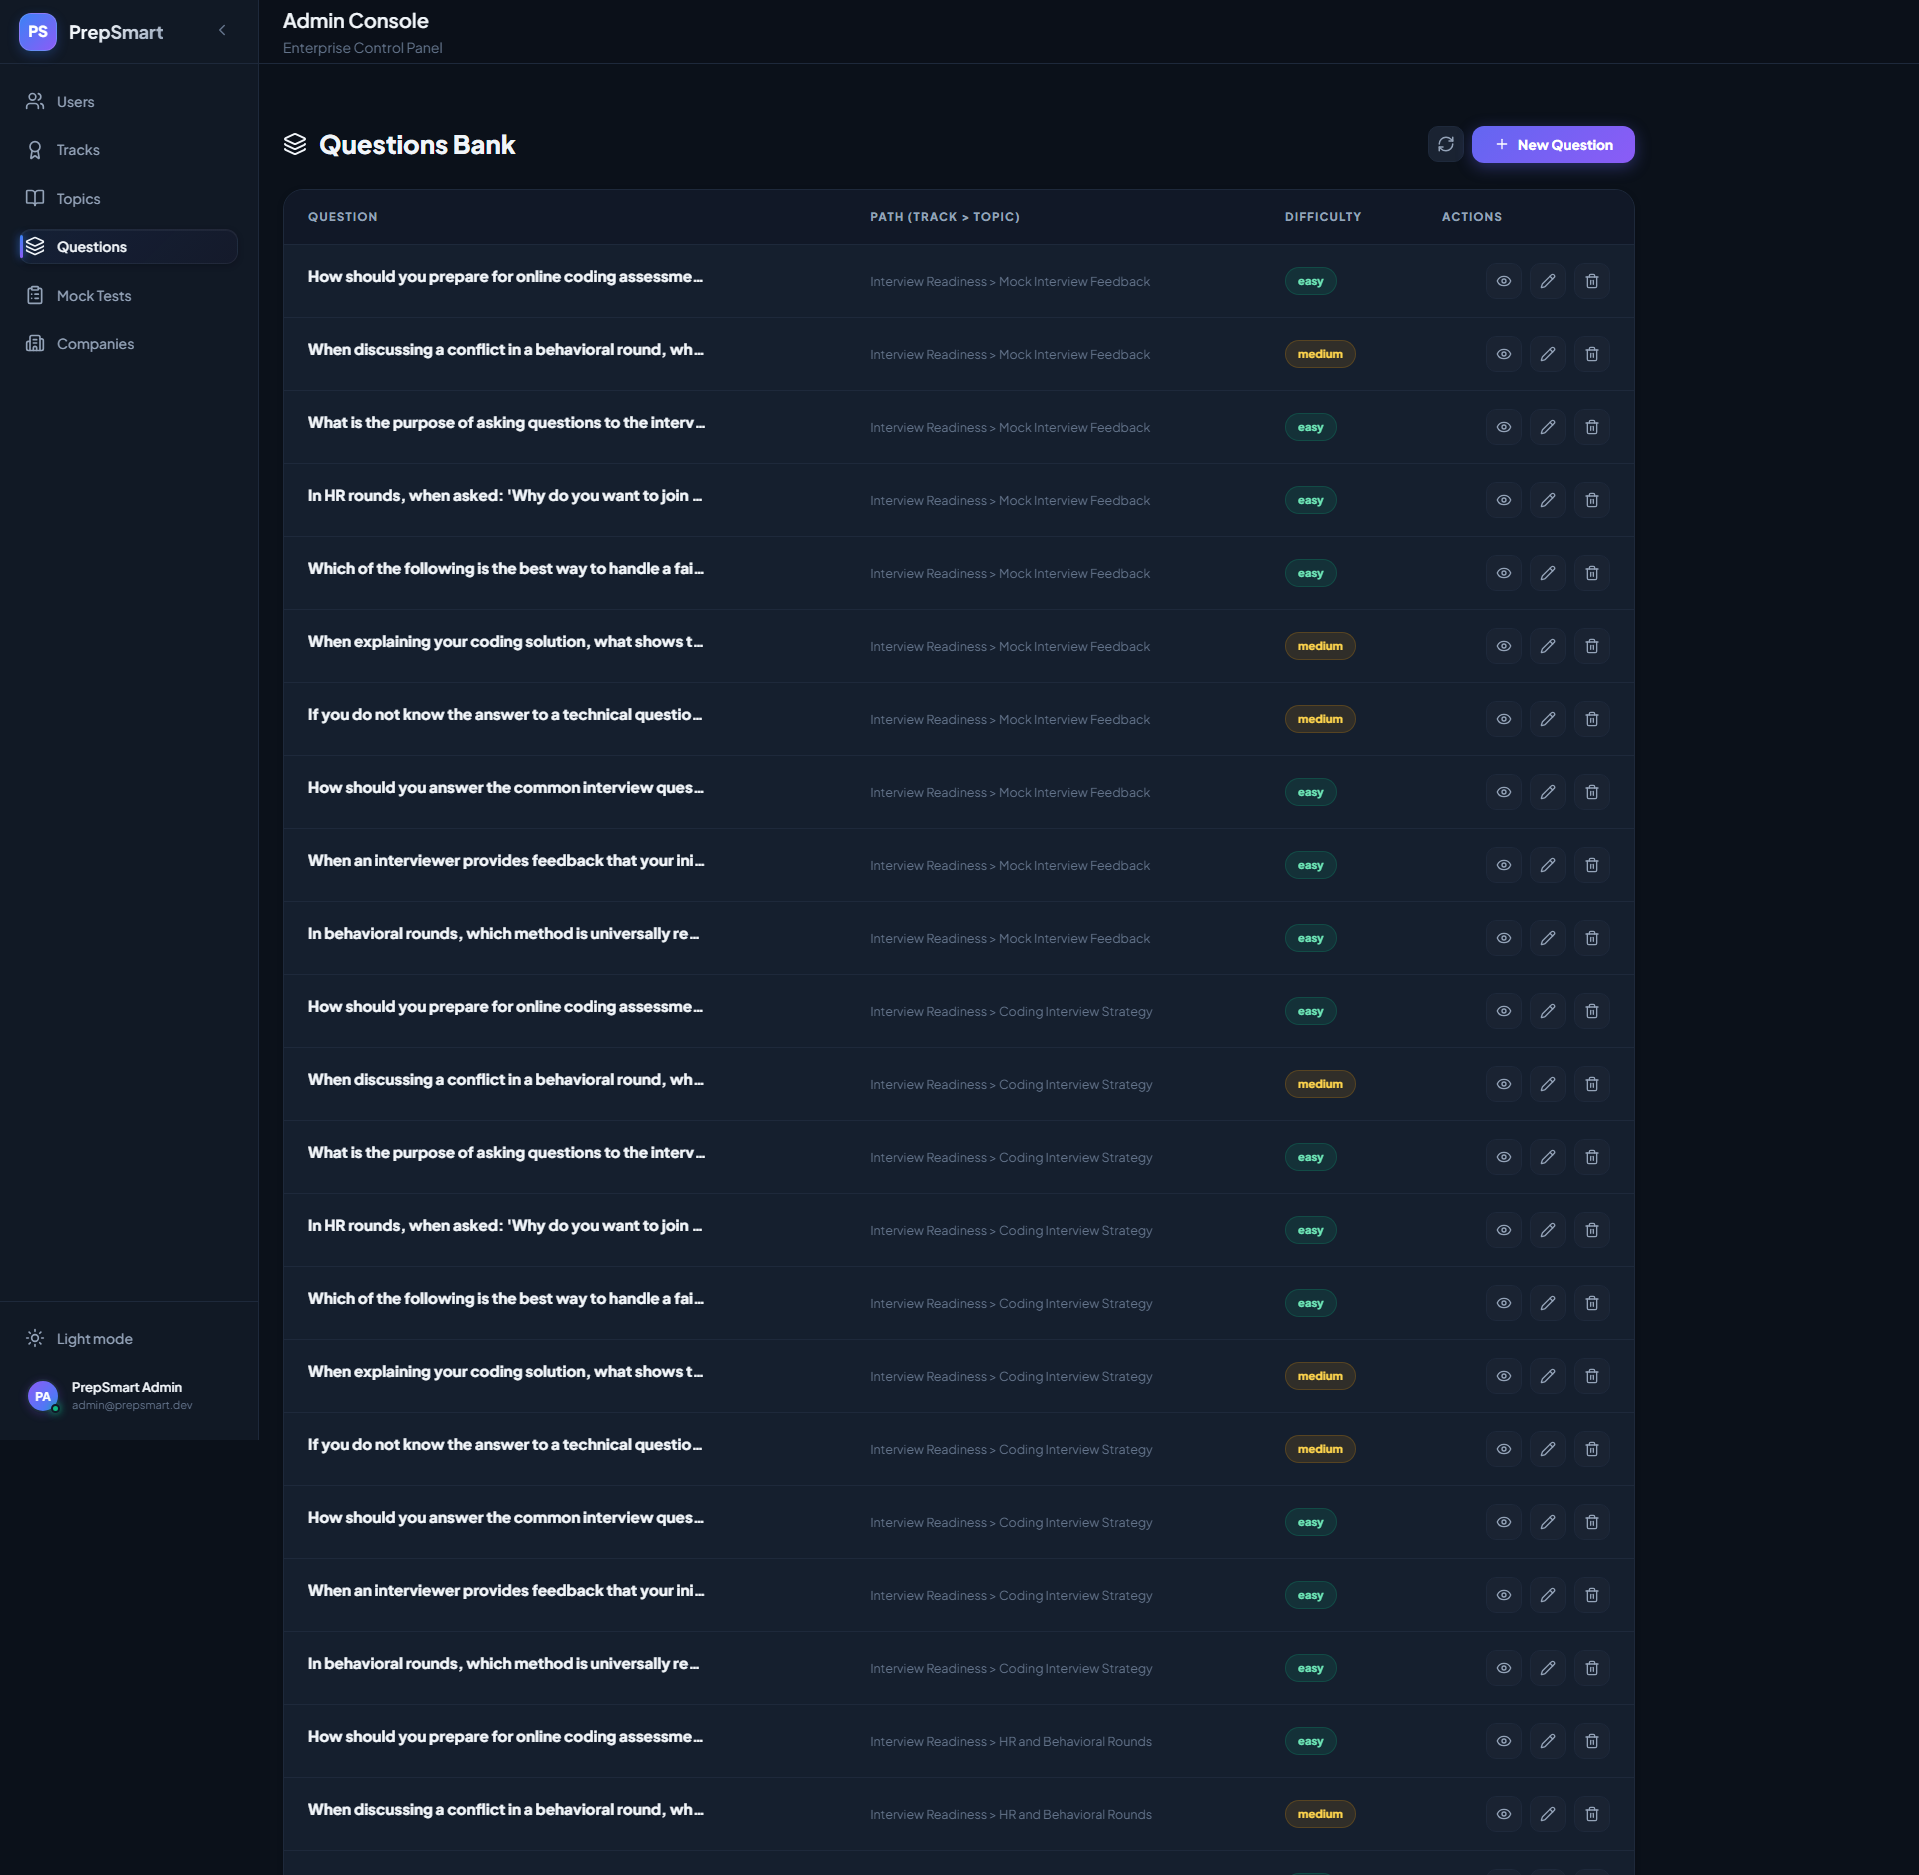
\includegraphics[width=0.90\textwidth]{Media/Chapter 5/admin_questions.png}
\caption{Administration - Question Management}
\label{fig:admin_questions}
\end{figure}

Administrators can create, modify, and maintain multiple-choice questions used in quizzes, assessments, and mock tests through this interface.

\subsection{Test Management}

\begin{figure}[H]
\centering
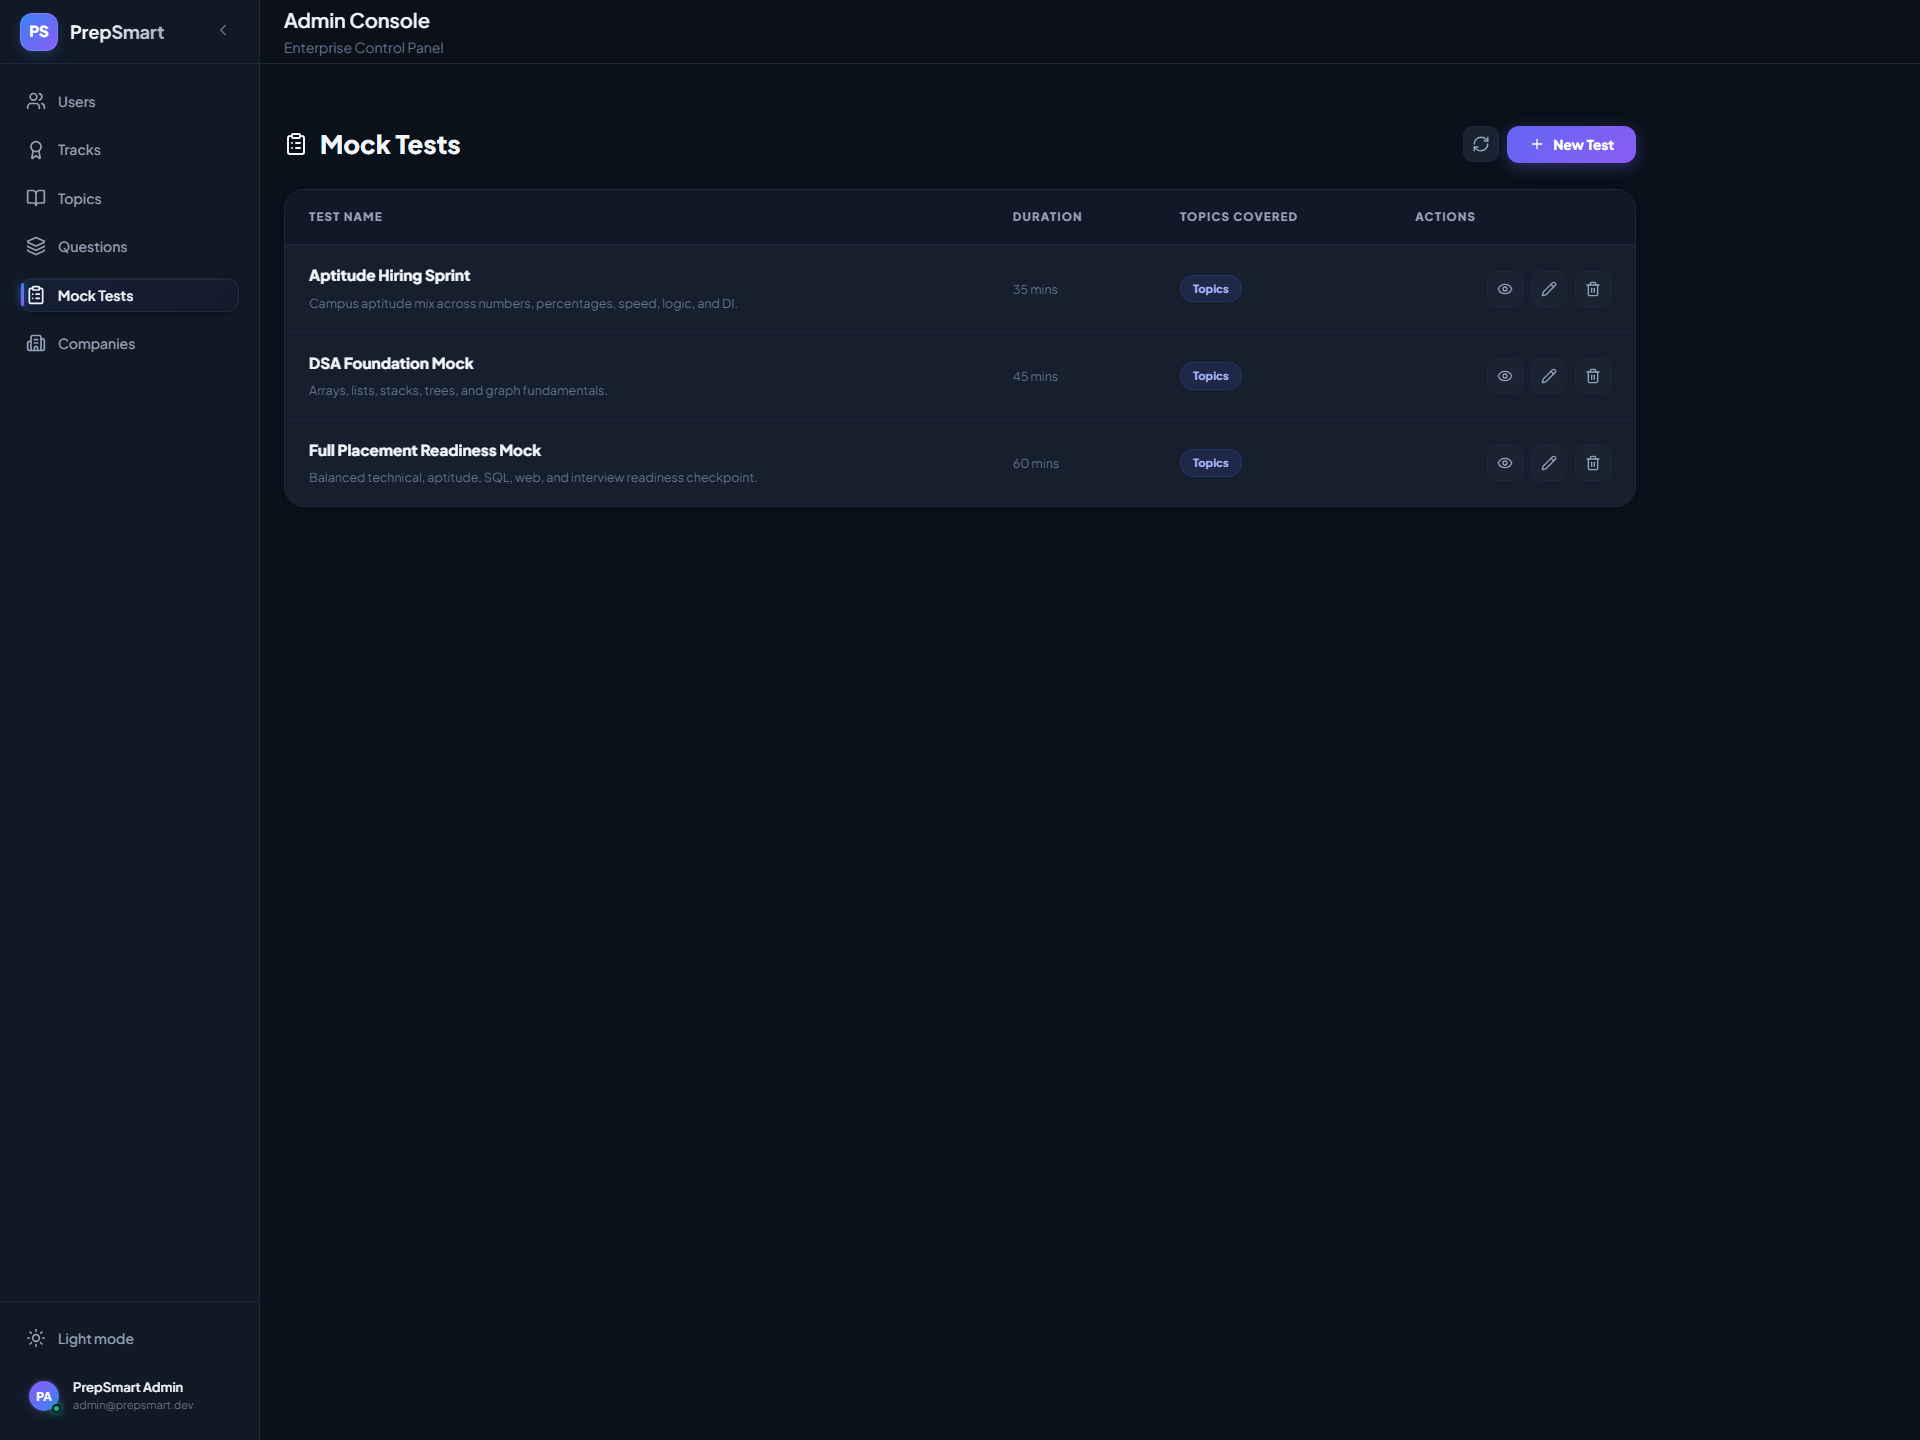
\includegraphics[width=0.90\textwidth]{Media/Chapter 5/admin_tests.png}
\caption{Administration - Test Management}
\label{fig:admin_tests}
\end{figure}

The Test Management interface allows administrators to configure mock tests, associate questions with assessments, and manage evaluation content for placement preparation.

\subsection{Company Management}

\begin{figure}[H]
\centering
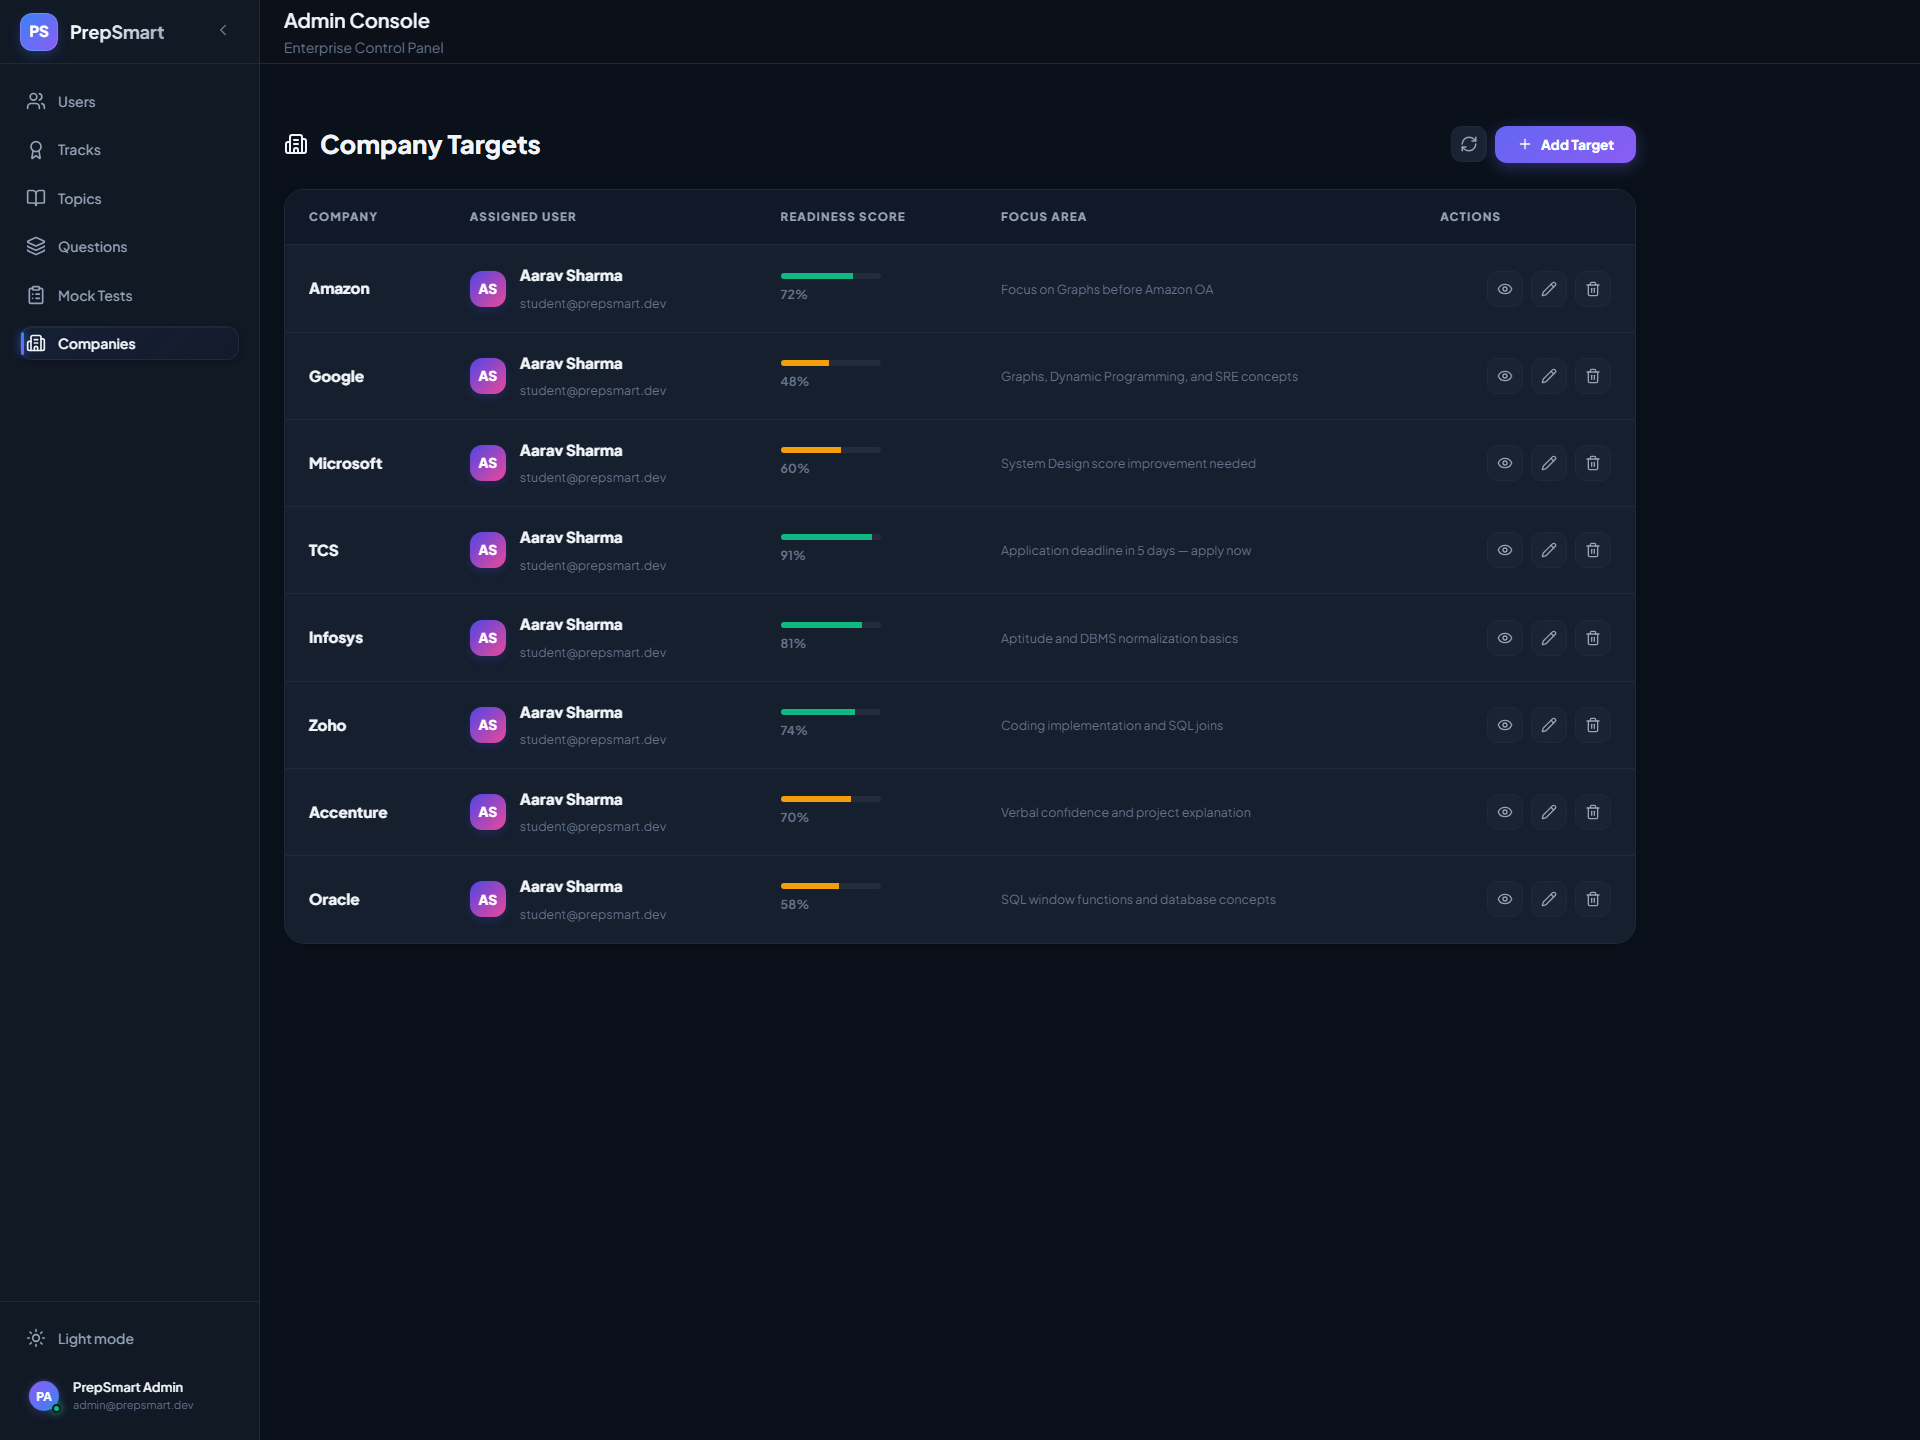
\includegraphics[width=0.90\textwidth]{Media/Chapter 5/admin_companies.png}
\caption{Administration - Company Management}
\label{fig:admin_companies}
\end{figure}

This interface enables administrators to maintain company-specific preparation information, readiness criteria, interview expectations, and recommended learning resources.

\subsection*{Major Features of the Administration Module}

\begin{itemize}

\item User account management.

\item Learning track administration.

\item Topic and content management.

\item Question bank maintenance.

\item Mock test administration.

\item Company information management.

\item Centralized platform administration.

\end{itemize}

\section{Chapter Summary}

This chapter presented the developed user interfaces of the PrepSmart platform and demonstrated the practical implementation of its major modules through screenshots. The chapter covered the landing page, user authentication, dashboard, placement preparation module, coding practice environment, AI interview module, company preparation module, profile management, shared profiles, analytics dashboard, settings, and administration module.

The presented interfaces demonstrate that PrepSmart successfully integrates multiple placement preparation activities into a single, user-friendly web application. The combination of modern user interface design, responsive layouts, real-time analytics, AI-assisted learning, and centralized management provides students with a comprehensive platform for effective placement preparation.

The next chapter discusses the overall conclusions of the project, summarizes the achieved objectives, identifies existing limitations, and presents possible directions for future enhancements.
    \chapter{Conclusion and Future Scope}

\section{Introduction}

This chapter presents the overall outcome of the Smart Placement Preparation Platform (PrepSmart) project. It summarizes the objectives achieved during development, discusses the major contributions of the proposed system, identifies its current limitations, and outlines possible enhancements that can be incorporated in future versions of the platform.

The development of PrepSmart demonstrates the successful integration of multiple placement preparation activities into a single web-based application. By combining structured learning, coding practice, AI-assisted interview preparation, company readiness analysis, portfolio generation, and analytical dashboards, the platform provides students with a comprehensive environment for campus placement preparation.

\section{Conclusion}

The primary objective of the PrepSmart project was to develop an integrated placement preparation platform capable of supporting students throughout their campus recruitment journey. The developed system successfully combines multiple preparation activities that are traditionally distributed across different websites into a unified application.

The platform provides structured learning paths, topic-wise study material, coding practice, mock assessments, AI-assisted interview preparation, company-specific readiness analysis, portfolio generation, skills passport creation, and analytical dashboards. These modules work together to simplify placement preparation while enabling students to continuously monitor their progress and identify areas requiring improvement.

The application has been developed using modern web technologies, including React for the frontend, Django REST Framework for backend services, MySQL for data storage, and JSON Web Tokens (JWT) for secure authentication. The modular architecture adopted during development improves maintainability, scalability, and future extensibility.

The implementation demonstrates that integrating learning resources, coding environments, analytics, and AI-assisted features into a single platform significantly improves the organization and efficiency of placement preparation. Therefore, the proposed system successfully satisfies the objectives identified during the requirement analysis phase.

\section{Objectives Achieved}

The developed system successfully achieves the major objectives established during the planning phase of the project.

\begin{itemize}

\item Developed a centralized placement preparation platform.

\item Implemented secure user authentication using JWT.

\item Provided structured learning paths for technical subjects.

\item Integrated coding practice within the application.

\item Developed mock tests and assessment modules.

\item Implemented AI-assisted interview preparation.

\item Provided company-specific preparation tracking.

\item Generated Skills Passport and professional portfolio.

\item Implemented personalized dashboards and analytics.

\item Developed an administrator module for content management.

\end{itemize}

\section{Current Limitations}

Although the developed platform provides comprehensive placement preparation support, certain limitations remain.

\begin{itemize}

\item The AI interview module depends on external AI services.

\item The code execution environment currently supports a limited number of programming languages.

\item Company preparation information is based on predefined datasets and requires periodic updates.

\item The platform has primarily been evaluated in an academic environment and has not yet undergone large-scale production deployment.

\item Certain advanced recommendation features can be further improved using machine learning techniques.

\end{itemize}

\section{Future Scope}

The PrepSmart platform provides a strong foundation for future enhancements. Several advanced features can be incorporated to further improve placement preparation and learning personalization.

Future improvements may include:

\begin{itemize}

\item Integration of adaptive AI-based learning recommendations.

\item Support for additional programming languages and online code execution environments.

\item Real-time collaborative coding interviews.

\item Video-based AI mock interviews.

\item Automatic resume evaluation using Artificial Intelligence.

\item Integration with LinkedIn and GitHub profiles.

\item Personalized placement recommendations using machine learning.

\item Cloud deployment for large-scale institutional use.

\item Mobile application development for Android and iOS platforms.

\item Integration with Learning Management Systems (LMS).

\end{itemize}

\section{Chapter Summary}

This chapter summarized the successful development of the PrepSmart platform and demonstrated that the proposed objectives were achieved through the implementation of an integrated placement preparation ecosystem. The developed application combines learning resources, coding practice, interview preparation, analytics, and company-specific guidance within a single web-based platform.

The identified limitations provide opportunities for future research and development, while the proposed enhancements demonstrate the potential scalability and long-term applicability of the system for educational institutions and students preparing for campus placements.



    \renewcommand{\bibname}{References}
    \newpage
    \phantomsection
    \addcontentsline{toc}{chapter}{References}
    \begin{thebibliography}{99}

\bibitem{react}
React Documentation, Meta Platforms Inc. [Online]. Available: \url{https://react.dev/}

\bibitem{django}
Django Documentation, Django Software Foundation. [Online]. Available: \url{https://docs.djangoproject.com/}

\bibitem{drf}
Django REST Framework Documentation. [Online]. Available: \url{https://www.django-rest-framework.org/}

\bibitem{mysql}
MySQL Documentation, Oracle Corporation. [Online]. Available: \url{https://dev.mysql.com/doc/}

\bibitem{jwt}
JSON Web Token (JWT) Introduction. [Online]. Available: \url{https://jwt.io/introduction/}

\bibitem{mdn}
MDN Web Docs (HTML, CSS, JavaScript). [Online]. Available: \url{https://developer.mozilla.org/}

\bibitem{python}
Python Documentation. [Online]. Available: \url{https://docs.python.org/3/}

\bibitem{github_prepsmart}
GitHub Repository (PrepSmart Project). [Online]. Available: \url{https://github.com/neeraj-cseh/Project}

\bibitem{stackoverflow}
Stack Overflow Developer Community. [Online]. Available: \url{https://stackoverflow.com/}

\bibitem{postman}
Postman API Documentation. [Online]. Available: \url{https://learning.postman.com/}

\bibitem{chatgpt}
ChatGPT, OpenAI. [Online]. Available: \url{https://chat.openai.com/}

\bibitem{codex}
OpenAI Codex, OpenAI. [Online]. Available: \url{https://chatgpt.com/codex/}

\bibitem{gemini}
Gemini AI, Google DeepMind. [Online]. Available: \url{https://gemini.google.com/}

\bibitem{claude}
Claude AI, Anthropic. [Online]. Available: \url{https://claude.ai/}

\bibitem{youtube_tuts}
YouTube Tutorials (Various Channels). [Online]. Available: \url{https://www.youtube.com/}

\end{thebibliography}

    \phantomsection
    \addcontentsline{toc}{chapter}{Supervisor Evaluation of Intern}

    \phantomsection
    \addcontentsline{toc}{chapter}{Student Feedback of Internship}

    \phantomsection
    \addcontentsline{toc}{chapter}{Plagiarism Report}

    \phantomsection
    \addcontentsline{toc}{chapter}{Daily Logs}

\end{document}
